\documentclass{book}[11pt]

\usepackage{bc}
\usepackage{epsfig}
\usepackage{url}
\usepackage{fullpage}
\usepackage{amsmath,amsfonts,amssymb,amscd,amsthm,xspace}
\usepackage{graphicx}
\usepackage{epstopdf}
\usepackage{booktabs}
\usepackage{rotating}
\usepackage{listings}
\usepackage{lstpatch}
\usepackage[centerlast,small,sc]{caption}
\usepackage{varwidth}
\usepackage{rotating}
\usepackage{colortbl}
\usepackage[table]{xcolor}
\usepackage{pdflscape}
\usepackage{pbox}
\usepackage[square, numbers, comma, sort&compress]{natbib}
\usepackage[pdfpagemode={UseOutlines},bookmarks=true,bookmarksopen=true,
bookmarksopenlevel=0,bookmarksnumbered=true,hypertexnames=false,
%colorlinks,linkcolor={blue},citecolor={blue},urlcolor={red},
colorlinks,linkcolor={black},citecolor={black},urlcolor={black},
pdfstartview={FitV},unicode,breaklinks=true]{hyperref}
\usepackage{xcolor}

\setcounter{secnumdepth}{3}
   
\graphicspath{ {./Figures/} }
\hypersetup{urlcolor=black, colorlinks=true}

\makeatletter
\newcommand{\thickhline}{\noalign {\ifnum 0=`}\fi \hrule height 1pt\futurelet \reserved@a \@xhline}
\newcolumntype{"}{@{\hskip\tabcolsep\vrule width 1pt\hskip\tabcolsep}}
\makeatother

\newcommand{\tab}{\hspace*{2em}}

\newcommand\todo[1]{\textcolor{red}{\textbf{{\tt TODO: #1}}}}

\begin{document}

  \thesistitle{Tunning the Blender Physics Engine via a Genetic Algorithm}{David Lettier}{\today}

  \newpage
  
  \pagenumbering{roman}
  
  %----------------------------------------------------------------------------------------
  %	THESIS CONTENT - ACKNOWLEDGMENTS
  %----------------------------------------------------------------------------------------
  
  \section*{Acknowledgments}
  
  Dr. Elizabeth Sklar's advisement was outstanding and pivotal to the work outlined below. Kudos to the computer science department for providing such an enriching master's program and enlisting exceptionally knowledgeable faculty. Additional kudos to the Blender and Bullet teams for developing a very robust platform for one to build off of.  

  \newpage
  
  %----------------------------------------------------------------------------------------
  %	THESIS CONTENT - ABSTRACT
  %----------------------------------------------------------------------------------------
  
  \section*{Abstract}
  
  %\todo{Write something about how the GA \textit{was} successful and how BlenderSim worked out.}

  Using a physics engine for robotic simulation provides fidelity with the added benefit of lower research costs, minimal space requirements, and even less time as the physical simulation can be run at faster than real-time speeds \cite{forklift}. However, physics engines have numerous parameters to tune such as friction coefficients, rigid-body constraints, body mass, gravitational acceleration, material elasticity, collision shapes, etcetera \cite{website:blender-rigidbody}\cite{website:blender-objecttype}. Tuning these either programmatically or as in the case of \textit{Blender}\footnote{Blender, released under the GNU General Public License, is a 3D creation suite allowing artists and programmers alike to produce immersive audio/visual works ranging from animation shorts to real-time 3D interactive games. Features include 3D modeling, 3D sculpting, texturing, sound editing, film editing, motion tracking, rigging, rendering, animation, physical simulation, a real-time 3D engine, and extensibility via the integrated Python API \cite{Hess:2007:EBG:1543288}.}---via the graphical user interface---is a daunting task considering the multidimensional state space. Simulation fidelity is compromised as some parameters are perfected while others are now maladjusted. Adjusting some parameters only to malign others leads to a ``herding cats'' type of effect. This ultimately results in a ``reality gap'' between the simulated environment and the physical environment. However, by using a genetic algorithm to optimize or rather fine tune the physics-engine parameters, the hypothesis was that the physics engine will produce a robot motion model more closely reassembling that of the real-world robot kinematics. This thesis documents a structured approach to tuning the Blender physics engine via a genetic algorithm thereby closing the reality gap between simulation and reality.  
  
  %----------------------------------------------------------------------------------------
  %	THESIS CONTENT - TOC
  %----------------------------------------------------------------------------------------

  \tableofcontents
  
  %----------------------------------------------------------------------------------------
  %	THESIS CONTENT - LOF
  %----------------------------------------------------------------------------------------

  \listoffigures
  
  %----------------------------------------------------------------------------------------
  %	THESIS CONTENT - LOT
  %----------------------------------------------------------------------------------------

  \listoftables

  \newpage
  \newpage
  \pagestyle{plain}
  \pagenumbering{arabic}
  \def\baselinestretch{1.9}
  \normalsize
  
  %----------------------------------------------------------------------------------------
  %	THESIS CONTENT - CHAPTERS
  %----------------------------------------------------------------------------------------

  \chapter{Introduction}

\label{Chapter1}

%\todo{Write this second to last.}

The motivation for thesis was inspired by the creation of a 3D simulator titled BlenderSim. Using Blender\footnote{Blender, released under the GNU General Public License, is a 3D creation suite allowing artists and programmers alike to produce immersive audio/visual works ranging from animation shorts to real-time 3D interactive games. Features include 3D modeling, 3D sculpting, texturing, sound editing, film editing, motion tracking, rigging, rendering, animation, physical simulation, a real-time 3D engine, and extensibility via the integrated Python API \cite{Hess:2007:EBG:1543288}.}, a 3D simulator was constructed for a human and robot multi-agent framework known as HRTeam \footnote{The purpose of HRTeam is to explore human and robot teamwork interactions \cite{hrteam}\cite{sklar-et-al-arms:2011}.}. By using BlenderSim, HRTeam experiments could be conducted in a real-time 3D physics-based virtual environment. The goal of BlenderSim was to provide a robust and high-fidelity simulation such that experimental results produced in simulation would be reproducible in reality.  

The physics engine employed by Blender, called Bullet\footnote{Bullet is the real time physics engine used by Blender. Released under the zlib license, Bullet provides real time continuous collision detection and rigid body dynamics \cite{website:continuousphysics}.}, proved to be troublesome while developing BlenderSim. The simulated robots would ``jitter'' erratically, fall through the floor, fly through the air, and/or fall apart even with no applied forces. Many days, turning into weeks, were lost trying to find the correct physics parameters by hand such that the simulation would produce high-fidelity results. In order to progress on the development of the BlenderSim 3D simulation environment, the idea of using the physics engine to model the motion of the robots was abandoned and a constant velocity motion model was used in its place. 

In the interim, the thesis problem was to tune the Blender physics engine via a genetic algorithm (GA) such that the physics engine would more closely model the motion of a real robot used in HRTeam experiments. This problem was approached in three incremental stages where each subsequent stage built off of the research and development done during the previous stage. Stage one involved the development a GA that tuned the weights of a neural network (NN) where the NN governed the movement of a paddle in a ``Pong''-like game titled SimPL. Using the GA developed in stage one, stage two tuned the Blender physics engine as it iteratively compared the motion of a simulated robot to motion data collected on a real robot. Lastly, with the physics engine tuned in stage two, stage three compared the motion of a simulated robot versus a real robot by simulating a previously conducted HRTeam experiment.           

\section{Genetic Algorithms}

Inspired by the theory of evolution, GAs attempt to solve problems that involve multidimensional state spaces \cite{ColinReeves}\cite{Beasley93anoverview}. GAs overcome problems experienced by other algorithms, such as hillclimbing, random search, or simulated annealing, by using a mixture of exploitation and exploration \cite{Beasley93anoverview}. Running in a loop, a GA generates proposed solutions to a problem, evaluates each proposed solution's value, and then capitalizes on what it learned to produce further potential solutions. Applications of GAs include numerical function optimization, image processing, combinatorial optimization, and civil engineering \cite{Beasley93anoverview}. What problems are appropriate for GAs and why GAs work when they do are highly debated topics with no dominant answers \cite{ColinReeves}. With so many variations and parameters values possible, no two GA implementations are guaranteed to be identical, ``...the number of variations that have been suggested is enormous. Probably everybody's GA is unique!'' \cite{ColinReeves}.

The term \textit{genetic algorithm} has both a strict and broad definition \cite{Whitley94agenetic}. The strict definition of a genetic algorithm is the model formally presented by John Holland in 1975 \cite{ColinReeves}. More generally, the broad definition is, ``any population-based model that uses selection and recombination operators to generate new sample points in a search space''\cite{Whitley94agenetic}. \textit{Genetic algorithm}, as it is used in this text, should be interpreted with the broad definition. Additional terms used require their own distinctions. \textit{Gene} refers to a single encoded value, representative of a dimension inherent to some multidimensional problem. \textit{Genes} are a collection of encoded values that represent a state in some multivariate state space. A \textit{Genome} specifies a data structure that contains genes and other types of data such as the genome's fitness. The \textit{population} of a GA is made up of genomes. The terms \textit{genotype} and \textit{phenotype} are interconnected. A genotype is represented by the genes of a genome. By expressing or rather decoding a genotype, a phenotype is constructed. Specifically for SimPL, the genotype was an encoding of the NN's weights and the phenotype was the paddle's movement, as dictated by the NN. For the software developed in stage two (known as BBAutoTune), the genotype was an encoding of the physics engine's parameters and the phenotype was the simulated robot's collision bounds and motion, as modeled by the physics engine.           

% in this text is used in the \textit{genetic algorithm}, \textit{gene}, \textit{genome}, \textit{genotype}, and \textit{phenotype} used in this thesis should be interpreted using the broad definition.

\section{SimPL}

Instead of diving right into the difficult problem targeted by the thesis, SimPL was an intermediate step to developing a GA capable of tuning a 3D physics engine. The problem for SimPL involved a NN and an on-screen paddle and ball. With the NN controlling the movement of the paddle, the GA developed for SimPL continuously tuned the weights of the NN. With each tuning of the weights, the NN became progressively better at controlling the paddle to hit the ball consistently. This simpler but still related problem provided a tractable context to conduct the needed background research of GAs. With the knowledge gained by solving the problem for SimPL, the thesis project was set up for success.    

\section{BBAutoTune}

The core work of the thesis was BBAutoTune. Using the SimPL GA as a base, the goal of BBAutoTune was to tune the Blender physics engine via a GA such that the physics engine would closely model the motion of a real robot used in HRTeam experiments.  With a few modifications, the SimPL GA was easily converted to handle the thesis problem. After collecting data on the motion of the real robot, BBAutoTune learned the necessary physics parameters needed to make the physics engine closely model the motion of the real robot. The motion of the real robot learned was its forward motion given a forward command.      

\section{BlenderSim}

% BlenderSim was a Blender based, 3D simulator developed for HRTeam during the summer of 2013. Initially, the physics engine in Blender was used to simulate the motion of the robots used in HRTeam experiments. However the physics engine was largely unusable and no amount of parameter tweaking provided consistent and stable results. Thus the physics engine was abandoned as the motion model and a constant velocity model was used in its place. As a proof-of-concept of the thesis, BlenderSim (and specifically the physics engine itself) was revisited using the tuned parameters found by BBAutoTune. By rerunning a previously run HRTeam experiment, the motion of the simulated, physics-based robot was compared with the motion of the real robot.

BlenderSim was a Blender based, 3D simulator developed for HRTeam during the summer of 2013. As a proof of concept of the thesis, BlenderSim (and specifically the physics engine itself) was revisited using the tuned parameters found by BBAutoTune. By rerunning a previously run HRTeam experiment, the motion of the simulated, physics-based robot was compared with the motion of the real robot. 


  \chapter{Genetic Algorithms}

\label{Chapter2}

\section{Overview}

Stub.

\section{Genomes}

Stub.

\subsection{Genes}

Stub.

\subsubsection{Encoding}

Stub.

\section{Evaluation}

Stub.

\subsection{Criteria}

Stub.

\subsection{Fitness Function}

Stub.

\subsection{Fitness Landscape}

Stub.

\section{Operators}

Stub.

\subsection{Selection}

Stub.

\subsection{Elitism}

Stub.

\subsection{Crossover}

Stub.

\subsection{Mutation}

Stub.

\section{Population}

Stub.

\subsection{Initialization}

Stub.

\subsection{Reproduction}

Stub.

\section{Termination}

Stub.

\subsection{Criteria}

Stub.

  \chapter{SimPL}

\label{Chapter3}

\section{Overview}

\todo{Change to past tense in regards to what was learned by SimPL.}

SimPL is an asymmetric autonomous pong clone with one paddle and one ball. SimPL is comprised of web-based technologies: HTML5, JavaScript, CSS, AJAX, MySQL, and PHP. At the time of this writing, SimPL can be viewed at http://www.lettier.com/simpl/. The paddle in SimPL is controlled by a feed-forward neural network. The neural network's weights are tuned via a genetic algorithm. 

The focus for SimPL was to learn about and to cultivate a genetic algorithm capable of tuning parameters with respect to a fitness landscape thereby producing an optimum solution to a given parameter space. The genetic algorithm developed for SimPL will be used as a basis for a genetic algorithm needed to solve a harder problem of tuning a 3D physics engine. 

\section{Implementation}

\subsection{Arena}

The arena for SimPL resides in a browser window. Four transparent walls reside at the top, right, bottom, and left of the screen. The arena contains a ball and paddle with the paddle affixed to the far left of screen and the ball originating from the far right of the screen. See Figure \ref{fig:arena}.

\begin{figure}[htbp]  
  \centering
  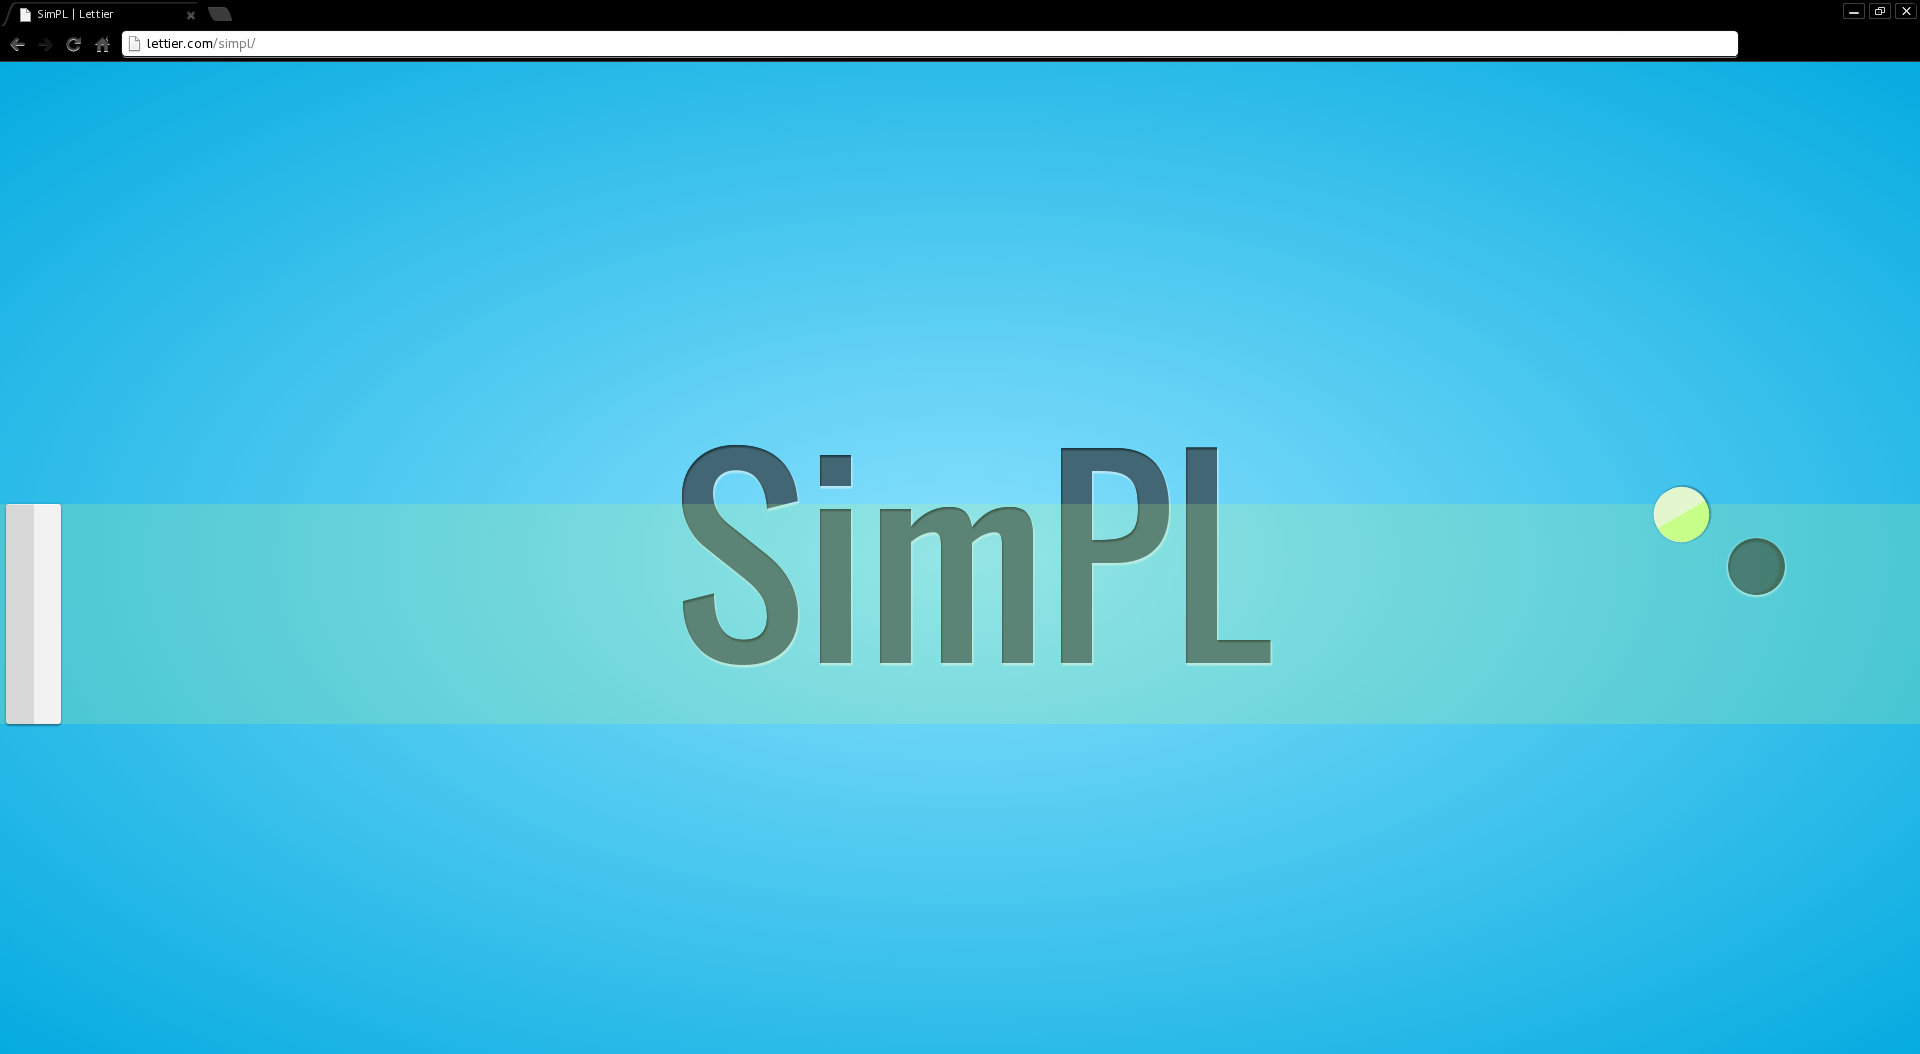
\includegraphics[scale=0.2]{../Figures/Chapter3/arena.png}
  \rule{35em}{0.5pt}
  \caption[SimPL Arena]{Here you see the SimPL arena containing the paddle and ball.}
  \label{fig:arena}
\end{figure}

\subsection{Ball}

The ball is a physics-based dynamic object. Its starting position and starting velocity magnitude are the same at the start of every round\footnote{A round is defined as the time from when the ball is launched from its starting position to either the time at which the ball leaves the left side of the arena or at the time in which the ball's velocity magnitude drops below $100$.}. Just before the beginning of a round, a random angle in the range $[135^\circ,225^\circ]$ is chosen as the ball's starting angle. See Figure \ref{fig:ball}. The ball's position is managed by the physics engine which responds to any collisions against the arena walls and/or the paddle.

\begin{figure}[htbp]  
  \centering
  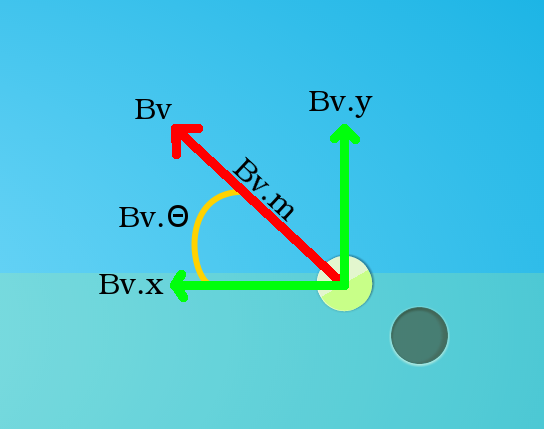
\includegraphics[scale=0.5]{../Figures/Chapter3/ball.png}
  \rule{35em}{0.5pt}
  \caption[SimPL Arena Ball]{Here you see the ball's dynamic physics properties.}
  \label{fig:ball}
\end{figure}

If the ball collides with the left wall, the round is over. Otherwise, if the ball collides with the top, right, or bottom wall, the ball is bounced back into the arena via its angle-of-reflection based on its collision angle-of-incidence. Collisions with the paddle work in the same fashion where the ball is bounced back via its angle-of-reflection based on its collision angle-of-incidence. See Figure \ref{fig:angle}.

\begin{figure}[htbp]  
  \centering
  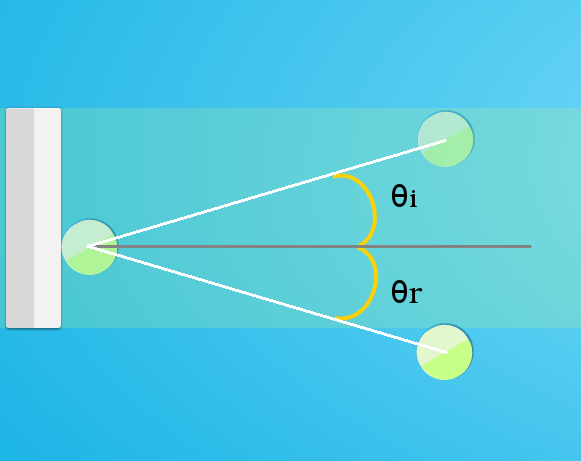
\includegraphics[scale=0.5]{../Figures/Chapter3/angle.png}
  \rule{35em}{0.5pt}
  \caption[SimPL Angle of Incidence]{Here you see the ball's collision angle-of-incidence $\theta_i$ and its angle-of-reflection $\theta_r$.}
  \label{fig:angle}
\end{figure}

Each collision the ball makes reduces its velocity magnitude. Let $m$ denote the ball's velocity magnitude. The formula used is $m = m - (m * 50\%)$. Once the ball's velocity magnitude drops below $100$ the round is over.

\pagebreak

\subsection{Paddle}

The paddle is a physics-based dynamic object that has a fixed velocity angle of either $90^\circ$ or $270^\circ$. See Figure \ref{fig:paddle}. Its starting position as well as its starting velocity magnitude are the same at the start of every round. 

\begin{figure}[htbp]
  \centering
  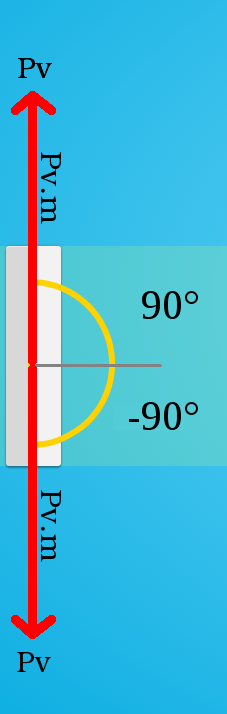
\includegraphics[scale=0.3]{../Figures/Chapter3/paddle.png}\\
  \rule{35em}{0.5pt}
  \caption[SimPL Paddle]{Here you see the paddle's dynamic physics properties.}
  \label{fig:paddle}
\end{figure}

The paddle's direction and speed are regulated by the output of the neural network. The output of the neural network is in the range $[-1,1]$. A neural network output of $0$ results in the paddle not moving from its current position. A neural network output in the range of $(0,1]$ results in the paddle traveling up by some percentage of its starting velocity magnitude. A neural network output in the range of $[-1,0)$ results in the paddle traveling down by some percentage of its starting velocity magnitude. For example, say the neural network output is $0.68$ and let $m$ denote the paddle's velocity magnitude. The paddle's velocity angle would be set to $90^\circ$ and its velocity magnitude would be set to $m_{new}=0.68*m_{initial}$ where $m_{initial}$ is the paddle's starting velocity magnitude (specifically $1000 \ \frac{pixels}{second}$). Here the paddle can always travel as fast or faster than the ball given that the starting velocity magnitude of the paddle and ball are the same at the start of every round. However, while ball's velocity magnitude is reduced after every collision the ball makes, the paddle has the possibility of always traveling as fast as it could at the start of the round (albeit depending on the neural-network output). Thus, it is never the case that the paddle does not have the possibility of never reaching the ball in time during the duration of any round. In other words, it is never the case that the neural-network outputs the correct movement---given the paddle's and ball's states---but the paddle misses out on fitness it could have gained had it been traveling fast enough to reach the ball. The paddle can always reach the ball given the neural network output is correct given the paddle's and ball's states. Thus, at any time $t$ during any round $R_i$, the paddle's velocity magnitude is $0\leq m \leq 1000 \ \frac{pixels}{second}$ as $m = \left|[-1,1]\right| * m_{initial}$ where $\left|[-1,1]\right|$ is the absolute value of the neural-network's output range.    

Collisions can occur for the paddle between the top wall, the bottom wall, and the ball. Collision with either the top or bottom wall results in the paddle's top or bottom being placed just before the wall. Collision with the ball results in no change of movement for the paddle---the paddle merely continues moving as it was before the collision occurred with the ball.

\subsection{Physics Engine}

All dynamic and static objects are registered with the physics engine before the first round. Once every draw loop of the SimPL game, the physics engine tests for collisions between dynamic objects and other dynamic objects and between dynamic objects and static objects. Those dynamic objects that are found to be colliding with either another dynamic object and/or static object are flagged as such and their collisions are handled accordingly. For those dynamic objects that are not colliding, their positions are updated based on their velocity.

\subsection{Neural Network}

The neural network is a feed-forward neural network that contains one input layer consisting of six input nodes, one hidden layer consisting of 5 hidden nodes, and one output layer consisting of one output node \cite{neuralnetworks}. Each threshold input to the hidden nodes and the output node is included among the weights of the network and thus are optimized or tuned via the genetic algorithm. In total, there are 41 weights ($(6+1)*5+(5+1)*1=41$) contained in the network. See Figure \ref{fig:nn}. Thus, there are 41 genes per genome in the genetic algorithm's population. All output from the hidden nodes and the output node are run through a sigmoid, hyperbolic-tangent-activation function $\left ( tanh(x)=\frac{e^{2x}-1}{e^{2x}+1} \right )$ resulting in an output range of $[-1,1]$.

\begin{figure}[htbp]  
  \centering
  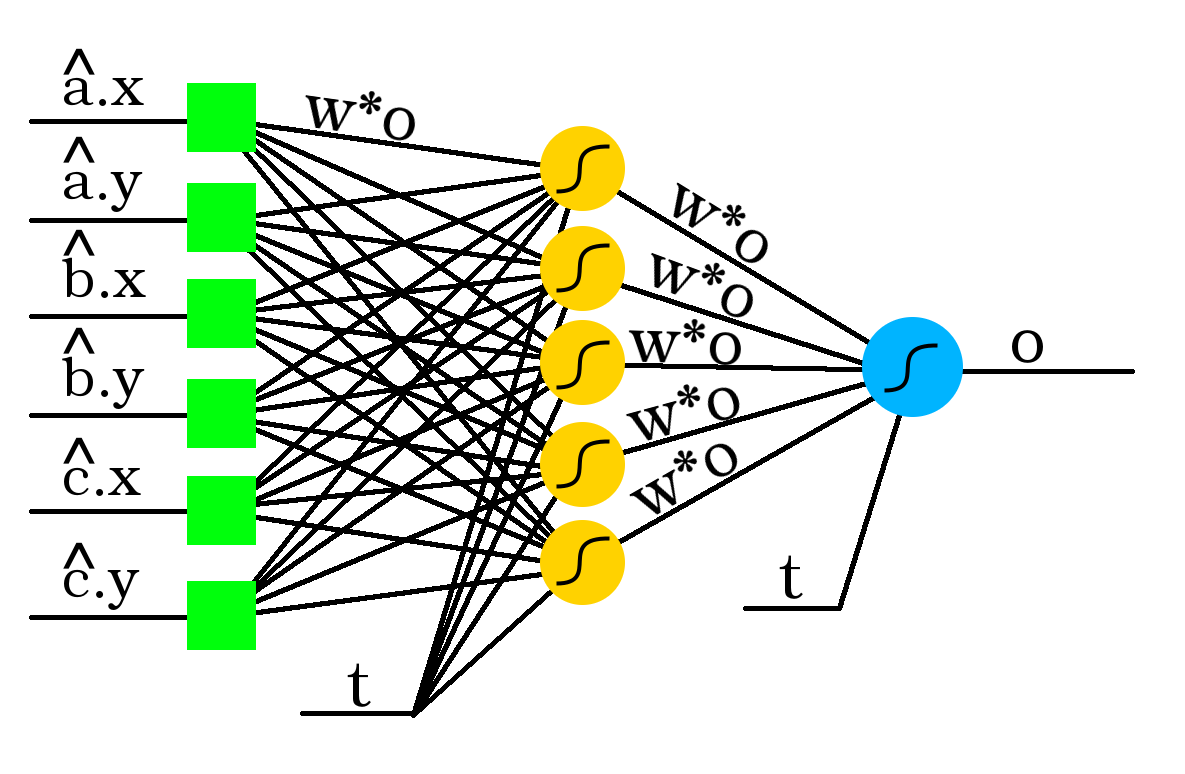
\includegraphics[scale=0.34]{../Figures/Chapter3/nn.png}
  \rule{35em}{0.5pt}
  \caption[SimPL NN]{Here you see the neural network as constructed in SimPL.}
  \label{fig:nn}
\end{figure}

Input to the neural network is normalized generating three unit vectors: from the ball's center to the paddle's center, the ball's velocity, and from the window's origin to the paddle's center. See Figure \ref{fig:unit_vectors}. These three unit vectors are broken down into their components resulting in six inputs to the neural network. See Figure \ref{fig:nn_input}. 

\begin{figure}[htbp]  
  \centering
  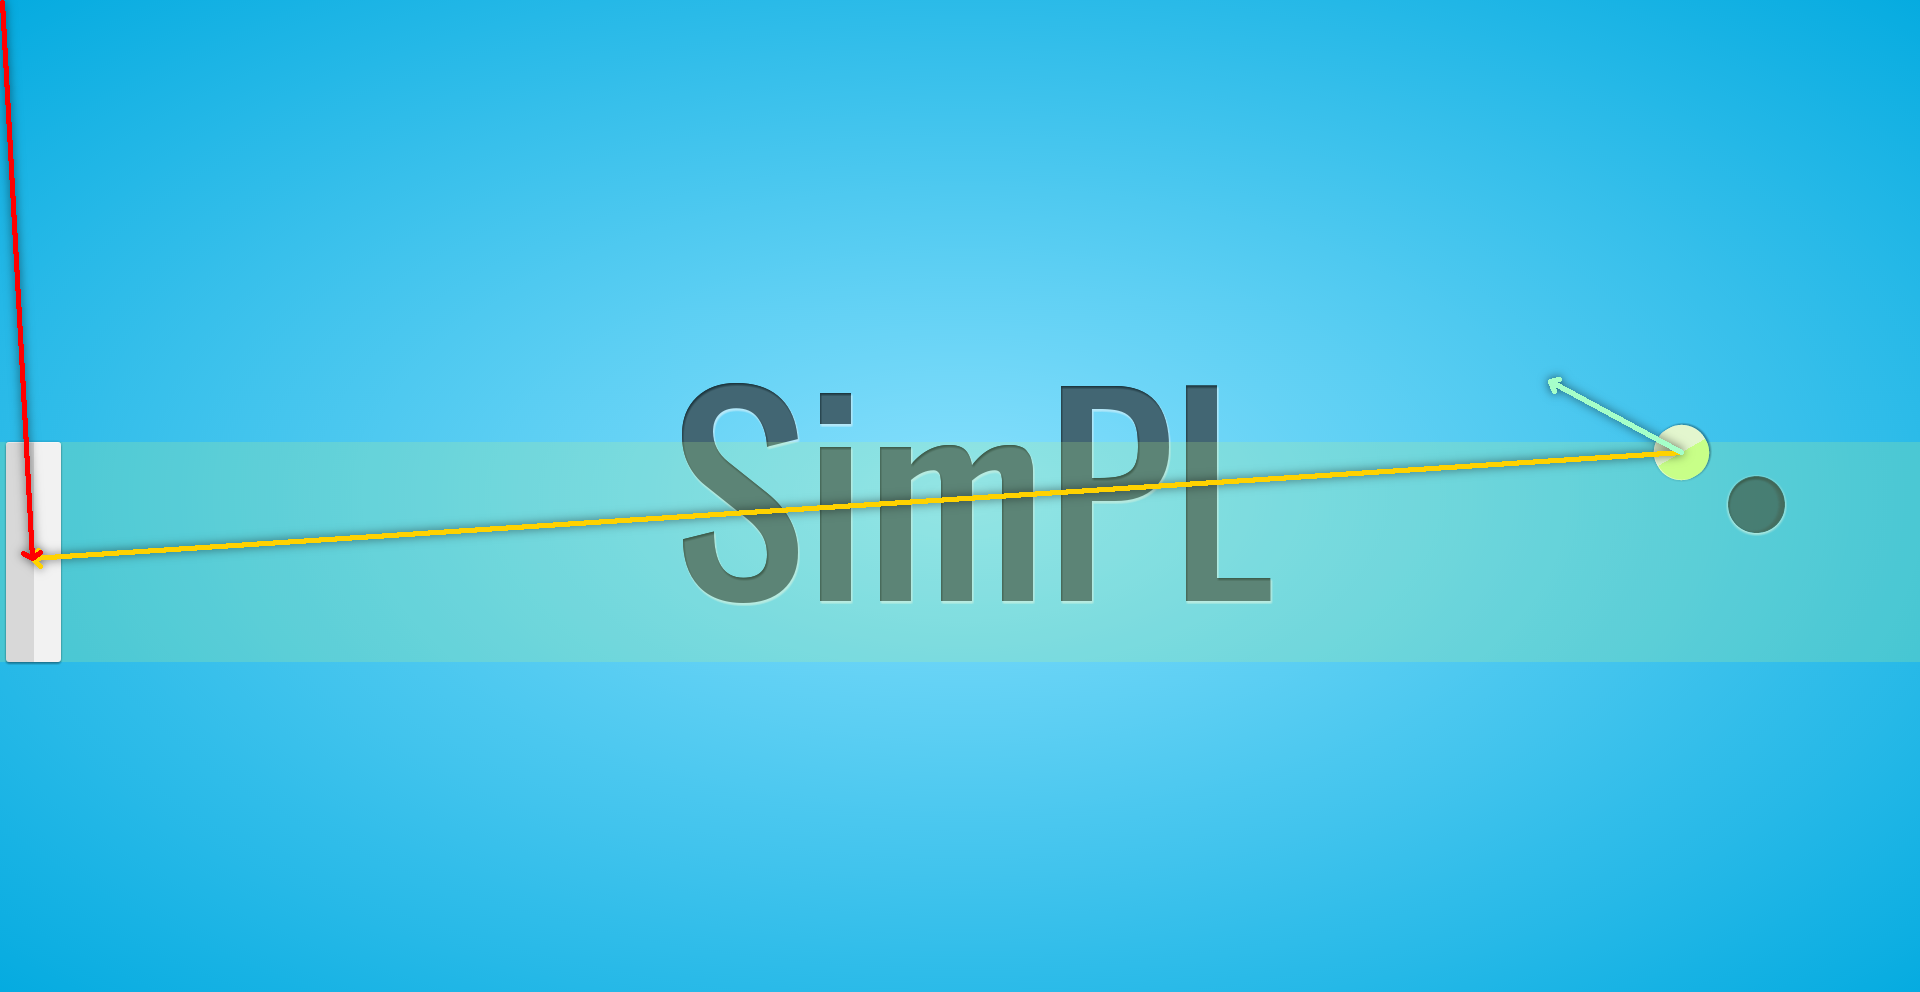
\includegraphics[scale=0.21]{../Figures/Chapter3/unit_vectors.png}
  \rule{35em}{0.5pt}
  \caption[SimPL NN Input Vectors]{Here you see the three input vectors to the neural network. Note that these vectors are normalized thereby turning them into unit vectors.}
  \label{fig:unit_vectors}
\end{figure}

\begin{figure}[htbp]  
  \centering
  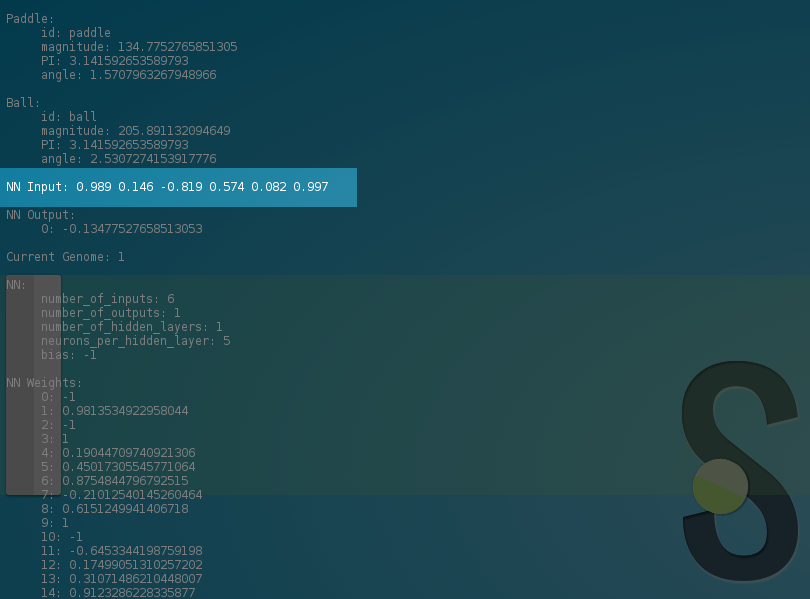
\includegraphics[scale=0.5]{../Figures/Chapter3/nn_input.png}
  \rule{35em}{0.5pt}
  \caption[SimPL NN Input Tuple]{Here you see the normalized input to the neural network.}
  \label{fig:nn_input}
\end{figure}

\pagebreak

\subsection{Genetic Algorithm}

\todo{Consider moving most of this to the GA chapter and only leave what was specific to SimPL.}

Instead of using back-propagation to train the weights of the neural network, a genetic algorithm is used to optimize or tune the weights of the neural network \cite{neuralnetworks}. The genetic algorithm consists of a population of genomes with each having a fitness property and an array of genes. For SimPL, the genes represent a solution of weights to be used in the neural network. Each genome is evaluated by a fitness function. As the genomes evolve over generations to produce fitter genomes, the neural network becomes increasingly accurate at outputting what the paddle should do (move up, stay still, or move down) based on the state of the ball and the paddle. 

The genetic algorithm contains four operators that work to produce fitter generations during the creation of a new population. The operators include: the elitism operator, the selection operator, the crossover operator, and the mutation operator. Initially, the genetic algorithm creates a random population of genomes. These initial genomes have zero fitness and a fixed number of genes. Each gene in every genome is given a random value sampled from a uniform distribution coinciding with some valid range. The genes are the input parameters to the mechanism the genetic algorithm is working to optimize. In the case of SimPL, the mechanism is the neural network and the parameters---of each genome---represent the 41 weights of the neural network. Each parameter has a valid range of $[-1,1]$. 

Once every genome in the population has been evaluated by the fitness function, the genetic algorithm constructs a new population from the previous generation. First, the elitism operator selects the $n$ fittest genomes from the old generation. These elite genomes are allowed to survive intact (however their fitnesses are reset to zero) and are placed into the new generation. Second, the genetic algorithm enters into a loop creating new genomes via the crossover operator and the mutation operator until an entirely new generation has been created. This new generation goes on to be evaluated as their predecessors were and the cycle repeats until some termination criteria is met. See Figure \ref{fig:ga}.

\renewcommand{\baselinestretch}{1.0}

\begin{figure}[htbp]
\begin{center}
\begin{varwidth}{\textwidth}
{\tt
BEGIN \\
\tab Generate a random population $P$ \\
\tab While not terminate do \\
\tab \tab Evaluate population $P$ \\
\tab \tab Create empty population $P'$ \\
\tab \tab Sort $P$ in order of fitness \\
\tab \tab Select $n$ fittest from $P$ and add them to $P'$ \\
\tab \tab While size of $P'$ $\leq$ population size do \\
\tab \tab \tab If perform crossover and mutation in sequence then \\
\tab \tab \tab \tab Select two genomes from $P$ \\
\tab \tab \tab \tab Generate two offspring via crossover with probability $C$ \\
\tab \tab \tab \tab Mutate the two offspring generated from crossover with probability $M$ \\
\tab \tab \tab \tab Add the generated offspring to $P'$ \\
\tab \tab \tab Else \\
\tab \tab \tab \tab Select two genomes from $P$ \\
\tab \tab \tab \tab Generate two offspring via crossover with probability $C$ \\
\tab \tab \tab \tab Add the offspring to $P'$ \\
\tab \tab \tab \tab Select one genome from $P$ \\
\tab \tab \tab \tab Mutate the selected genome with probability $M$ \\
\tab \tab \tab \tab Add the mutated offspring to $P'$ \\
\tab \tab \tab End if \\
\tab \tab End while \\
\tab \tab $P=P'$ \\
\tab End while \\
END \\
}
% \begin{equation*}
% \boxed{
% \begin{aligned}
% Begin \ GA: & \\
% &Generate \ population \ P_0. \\
% & While \ not \ terminate: \\
% & \quad\quad Evalute \ population \ P_i. \\
% & \quad\quad Create \ empty \ populutation \ P_{i+1}. \\
% & \quad\quad Sort \ P_i \ in \ non\!-\!decreasing \ order \ of \ fitness. \\
% & \quad\quad Select \ n \ fittest \ from \ P_i \ and \ append \ to \ P_{i+1}. \\
% & \quad\quad While \ |P_{i+1}| \ \leq \  population \ size: \\
% & \quad\quad\quad\quad If \ perform \ crossover \ and \ mutation \ in \ sequence: \\
% & \quad\quad\quad\quad\quad\quad g_1,g_2 \longleftarrow \ Select \ two \ genomes \ from \ P_i \ via \ roulette \ selection. \\
% & \quad\quad\quad\quad\quad\quad /\!* \ Generate \ two \ of\! fspring \ via \ crossover. *\!/ \\
% & \quad\quad\quad\quad\quad\quad o_1,o_2 \longleftarrow \ Crossover( g_1, g_2 ). \\
% & \quad\quad\quad\quad\quad\quad /\!* \ Mutate \ crossover's \ of\!fspring \ and \\
% & \quad\quad\quad\quad\quad\quad append \ to \ new \ population. \ *\!/ \\
% & \quad\quad\quad\quad\quad\quad P_{i+1} \longleftarrow \ P_{i+1} + Mutate( o_1, o_2 ). \\
% & \quad\quad\quad\quad Else: \\
% & \quad\quad\quad\quad\quad\quad g_1,g_2 \longleftarrow \ Select \ two \ genomes \ from \ P_i \ via \ roulette \ selection. \\
% & \quad\quad\quad\quad\quad\quad /\!* \ Generate \ two \ of\!fspring \ via \ crossover \\
% & \quad\quad\quad\quad\quad\quad and \ append \ to \ new \ population. \ *\!/  \\
% & \quad\quad\quad\quad\quad\quad P_{i+1} \longleftarrow \ P_{i+1} + Crossover( g_1, g_2 ). \\
% & \quad\quad\quad\quad\quad\quad /\!* \ Mutate \ the \ two \ selected \ genomes \\
% & \quad\quad\quad\quad\quad\quad and \ append \ to \ new \ population. \ *\!/  \\
% & \quad\quad\quad\quad\quad\quad P_{i+1} \longleftarrow \ P_{i+1} + Mutate( g_1, g_2 ). \\
% & \quad\quad P_{i} \longleftarrow P_{i+1}\\
% \end{aligned}
% }
% \end{equation*}
\end{varwidth}
\end{center}
\centering
\rule{35em}{0.5pt}
\caption[Basic GA]{Here you see the basic genetic algorithm.}
\label{fig:ga}
\end{figure}

\renewcommand{\baselinestretch}{1.9}

\vspace{3mm}

The selection operator uses roulette selection where the probability of some genome being selected is proportional to their fitness. Roulette selection and roulette selection with rank fitness was experimented with as outlined later \cite{geneticalgorithm}. The crossover operator takes two selected genomes to produce offspring where the offspring have some combination of their parents' genes. SimPL uses one-point crossover throughout each experiment. To select the crossover point per crossover operation, the crossover operator samples a random integer from a uniform distribution ($crossoverPoint = X\!\sim\!U(0,n-1)$ where $n$ is the number of genes per genome). The mutation operator takes a selected genome and mutates its genes using various means. If the mutation scope is at the gene level, the mutation operator traverses through the genome's gene array where for each gene, the mutation operator samples a random integer from a uniform distribution ($X\!\sim\!U(0,1)$) and if this random integer $X$ is less than or equal to the mutation probability, the mutation operator mutates the gene value either via uniform mutation ($geneValue_i = X\!\sim\!U(0,1) * \varepsilon$) or Gaussian mutation ($geneValue_i = X\!\sim\!N(\mu,\sigma^2)$). If the mutation scope is at the genome level, the mutation operator samples a random integer from a uniform distribution ($X\sim U(0,1)$) and if this random integer $X$ is less than or equal to the mutation probability, the mutation operator mutates all of the genome's gene values one after the other via either uniform mutation ($geneValue_i = X\!\sim\!U(0,1) * \varepsilon$) or Gaussian mutation ($geneValue_i = X\!\sim\!N(\mu,\sigma^2)$). These means of mutation were experimented with as outlined later. Crossover and mutation can be carried out in sequence or can be done separately with one operator not interfering the other operator's offspring. This was experimented with as outlined later.

Crossover and mutation are not guaranteed to always occur as the genetic algorithm produces new genomes from the old genomes. Rather, crossover and mutation occur based on some probability. If the crossover and mutation probabilities are both set to $1$ then they always occur. Before the genetic algorithm is initialized, the crossover and mutation probabilities are set \cite{self_adapt}. These initial crossover and mutation probability values can be arbitrary or can be based on some a-priori knowledge of the fitness landscape. The probabilities can change over time or can remain static throughout the run of the genetic algorithm. Different static settings and self-adaptation of the probabilities were experimented with as outlined later. 

The fitness function evaluates each genome in the current population based on some fitness criteria. The fitness criteria coincides with finding the optimum solution to the parameter space of the mechanism the genetic algorithm is producing fitter and fitter solutions to. For SimPL, the parameter space is the weights of the neural network. Each genome represents a solution or point in the weights space. An optimal solution in the weights space will make the neural network always give a correct output as to what movement the paddle must make based on the ball's and the paddle's current states. This will result in the paddle always following the ball or in other words, the paddle will never let the ball leave the left side of the screen. Thus the fitness criteria for SimPL could include how much or how well the paddle follows the ball and/or how many times the paddle hits the ball. Different fitness criteria were experimented with as outlined later. 

% GA loop
% crossover
% mutation
% observed rates
% perturbation
% Gaussian mutation
% whole versus gene-by-gene mutation
% sequential operators versus separate
% self-adaptation via tracking progress
% partial credit fitness

\subsection{Database Manager}

A database manager interfaces with a remote MySQL server either asynchronously or synchronously. Experiment data is recorded in the MySQL database as the experiment is carried out. Additionally, each generation produced by the genetic algorithm is logged to the database. Upon visiting the SimPL site, the last generation produced can be loaded into the genetic algorithm thereby allowing the simulation to pick up where it left off last.  

\section{Platform}

The browser window size has a significant influence over the fitnesses of the genomes being evaluated. While the arena fits to whatever size the browser window is, the size of the paddle and the ball do not directly change in proportion to the window size. Thus, a small browser window gives the paddle less screen real estate to cover in comparison to a large browser window. For example, imagine a browser window size with a height as large as the paddle's height. Here the paddle can never move---it always follows the ball and always hits the ball. Thus, the resulting fitnesses observed would be erroneously high. Therefore, all experiments were run using the same browser window size. 

%it is important to note what platform SimPL was run on when discussing experimental results---especially when comparing experimental results with one another. Care was taken to run experiments on the same platform when the experiments would be directly compared to one another. 

%The laptop's browser window size is $\sim70\%$ the size of the desktop browser window size (see Figure \ref{fig:platform_sizes}) and thus higher fitnesses are observed when comparing identical runs of the genetic algorithm performed on the laptop versus the desktop. On the desktop the paddle has $992-220=772$ pixels to traverse while on the laptop the paddle has $681-200=481$ pixels to traverse.

%\begin{figure}[H]  
%  \centering
%  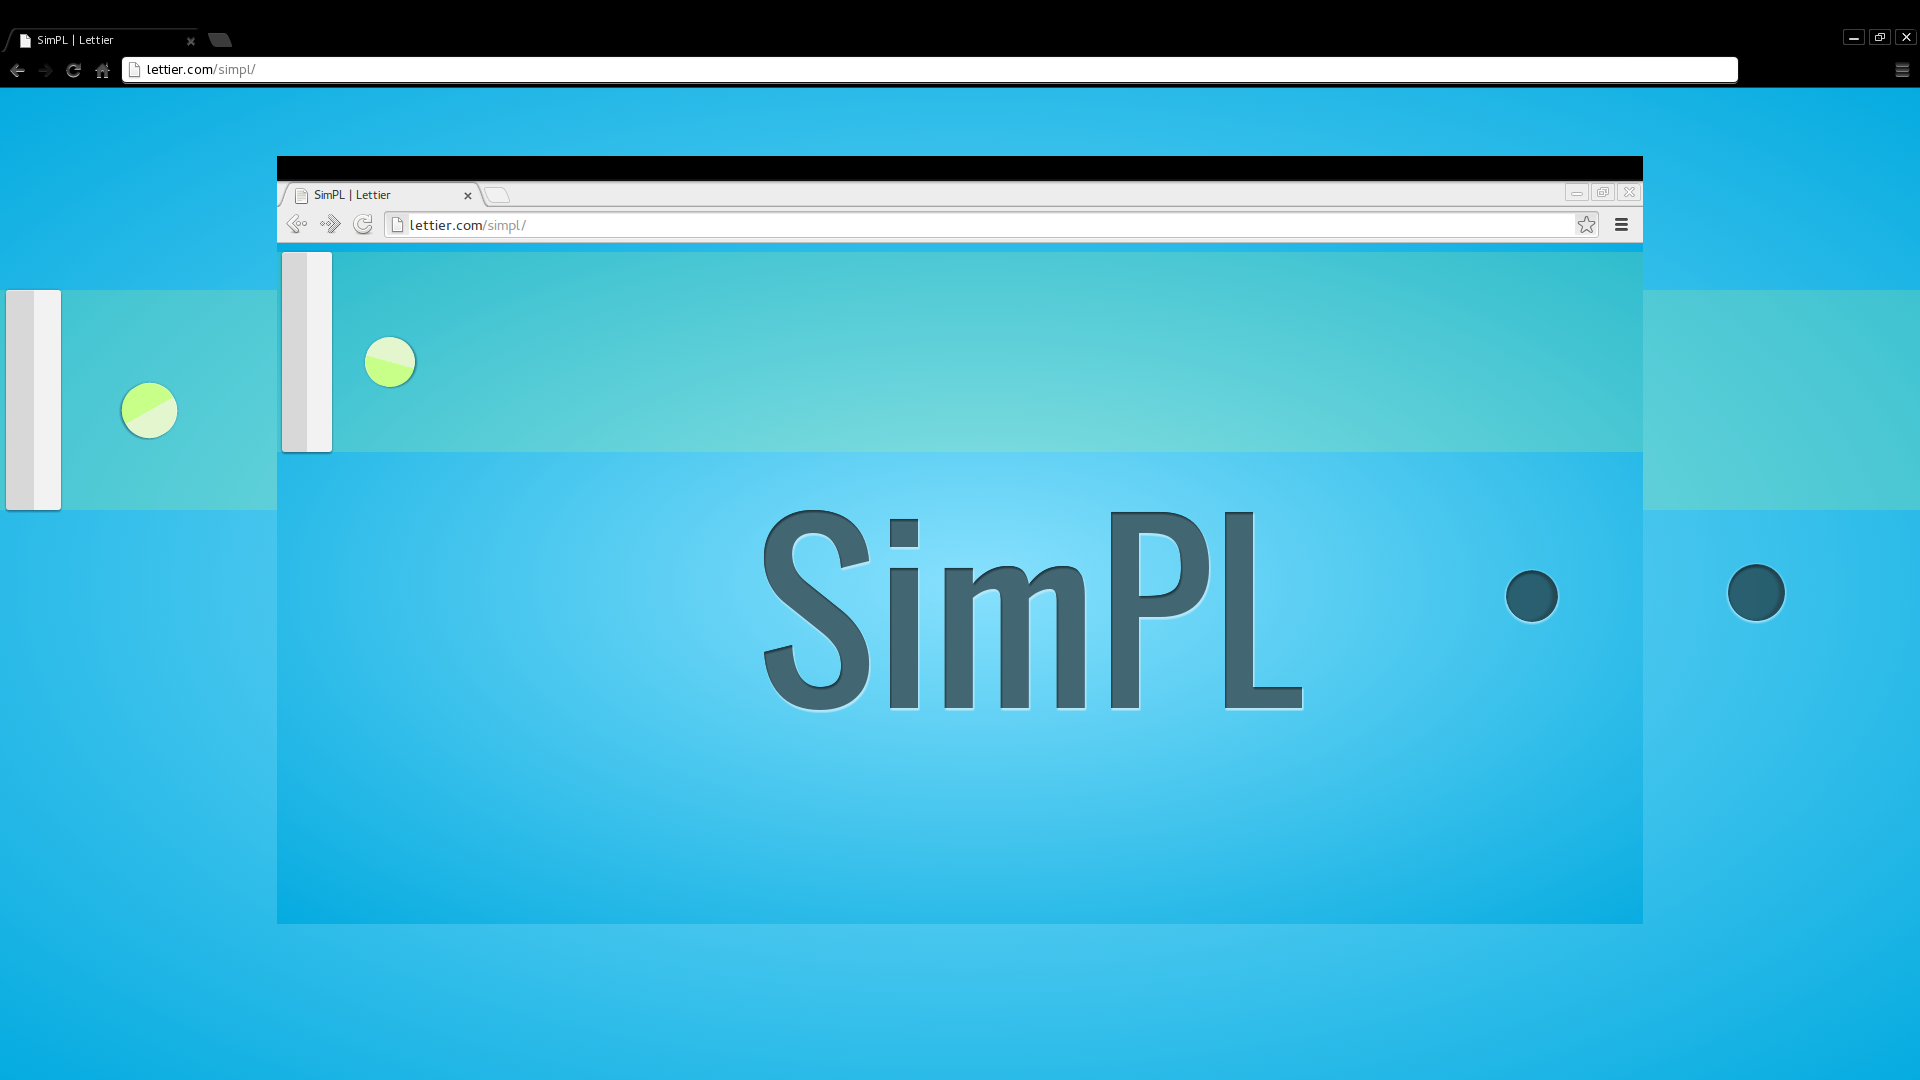
\includegraphics[width=.666\textwidth]{platform_sizes.png}
%  \caption{Here you see the laptop screen superimposed onto the desktop screen.}
%  \label{fig:platform_sizes}
%\end{figure}

%1526.3410497 / 2161.125632628  = 0.706271318

%\subsection{Desktop}

%Google Chrome version number 26.0.1410.63 was used on the desktop. Screen resolution was $1920\times1080$. Browser window size (both reported and actual) was 1920 pixels wide by 992 pixels tall. Paddle size reported (by the browser) was 50 pixels wide by 200 pixels tall but the actual size was 55 pixels wide by 220 pixels tall. Ball size reported (by the browser) was 50 pixels wide by 50 pixels tall but the actual size was 57 pixels wide by 57 pixels tall.

%\subsection{Laptop}
Experiments were run on a Lenovo Z580 Ideapad laptop running 64-bit Fedora 18 and was equipped with an Intel Core i5 CPU running at 2.5 GHz and 7.7 GiBs of memory. Google Chrome version number 30.0.1599.114 was used on the laptop. Screen resolution was $1366\times768$. Browser window size (both reported and actual) was 1366 pixels wide by 681 pixels tall. Paddle size reported (by the browser) was 50 pixels wide by 200 pixels tall and the actual size was the same. Ball size reported (by the browser) was 50 pixels wide by 50 pixels tall and the actual size was the same. The paddle had $681-200=481$ pixels of available screen-space to traverse.  

\section{Experimental Designs}

Each SimPL experimental design (with the exception of experiments six and seven) was constructed in such a way as to focus on a set of one or more facets to the genetic algorithm. See Table \ref{tab:exps}. With each progressive experiment, the facets not focused on were kept the same from the previous experiment. The goal was to create a genetic algorithm that would eventually---with efficiency---produce the optimal set of neural-network weights needed in order to generate a paddle that performs as well as the performance-standard paddle constructed in experiment six. Ultimately, the performance of any paddle in SimPL is how long it keeps the ball-in-play before the termination of any round.       

Experiments one and two revolved around the fitness function, the selection operator, and the static crossover and static mutation properties of the genetic algorithm. Experiments three, four, and five revolved around the self-adaptation of the crossover and mutation probabilities and whether allowing the mutation operator to disrupt the offspring, produced by the crossover operator, degraded the performance of the genetic algorithm. Experiment six revolved around constructing a paddle as an optimal-performance standard by which any other paddle could be measured by. Finally, experiment seven revolved around constructing a randomly behaving paddle thereby producing a performance lower bound.

For each experiment, the genetic algorithm was run for 100 generations where for each generation, the population's average fitness was recorded. Once every 10th generation, the current population's top performing genome was saved. After the run of the genetic algorithm was over, the saved top-performers were run in a tournament. This tournament consisted of running each top-performer for five rounds where for each top performer, the time in seconds they kept the ball-in-play per round was recorded. Once an every-10th-generation-top-performer was done with their five rounds, the average of their ball-in-play time per round was calculated and recorded.

\begin{landscape}
%\renewcommand*\arraystretch{1.5}
\begin{table}
%\hskip-1.7cm
%\footnotesize
\centering
    \begin{tabular}{ | >{\columncolor{lightgray}} r"c|c"c|c|c"c| } 
    \hline
    \rowcolor{lightgray} \textbf{GA Parameters $\times$ Experiment} & \textit{One} & \textit{Two} & \textit{Three} & \textit{Four} & \textit{Five} & \textit{Six \& Seven}  \\ \thickhline 
    \textit{Population Size} & 10 & 10 & 10 & 10 & 10 & 10 \\ \hline 
    \textit{Fitness Function Type} & \cellcolor{blue!25} Partial/Full & \cellcolor{blue!25} Full & Full & Full & Full & Full \\ \hline
    \textit{Number of Elite Offspring} & 2  & 2 & 2 & 2 & 2 & 10  \\ \hline
    \textit{Roulette Selection - Actual Fitness} & True & \cellcolor{blue!25} False  & False & False & False & N/A \\ \hline
    \textit{Roulette Selection - Rank Fitness} & False & \cellcolor{blue!25} True & True & True & True & N/A \\ \hline
    \textit{Sequential Crossover \& Mutation} & True & True & \cellcolor{blue!25} False & False & \cellcolor{blue!25} True & N/A \\ \hline
    %\textit{Parents Survive} & True & True & \cellcolor{blue!25} False & False & False & N/A \\ \hline
    \textit{Self-adaptation} & False & False & \cellcolor{blue!25} True & \cellcolor{blue!25} False & False &  N/A \\ \hline
    \textit{Crossover Type} & One-point & One-point & One-point & One-point & One-point & N/A \\ \hline
    \textit{Crossover Probability }& 0.7 & \cellcolor{blue!25} 0.8 & \cellcolor{blue!25} 0.5 & \cellcolor{blue!25} 0.7816 & 0.7816  & N/A \\ \hline
    \textit{Mutation Type} & Uniform & \cellcolor{blue!25} Gaussian & Gaussian & Gaussian & Gaussian &  N/A \\ \hline
    \textit{Mutation Scope} & Gene & Gene & \cellcolor{blue!25} Genome & Genome & \cellcolor{blue!25} Gene & N/A \\ \hline
    \textit{Mutation Probability } & 0.1 & \cellcolor{blue!25} $\left(\frac{1}{n}\right)=\left(\frac{1}{41}\right) \approx 0.0244$ & \cellcolor{blue!25} 0.5 & \cellcolor{blue!25} 0.2184 & 0.2184 & N/A \\ \hline
    \textit{Mutation Step} & $X\sim U(0,1) * 0.3$ & \cellcolor{blue!25} $X\sim N(\mu,\sigma^2)$ & $X\sim N(\mu,\sigma^2)$ & $X\sim N(\mu,\sigma^2)$ & $X\sim (\mu,\sigma^2)$ & N/A \\ \hline
    \textit{Mutation Step} $\mu$ & N/A & \cellcolor{blue!25} Gene Value & Gene Value  & Gene Value  & Gene Value & N/A \\ \hline
    \textit{Mutation Step} $\sigma$ & N/A & \cellcolor{blue!25} 0.5 & \cellcolor{blue!25} $M_{Prob.}$ & $M_{Prob.}$ & $M_{Prob.}$ & N/A \\ \hline
    \end{tabular}
\caption[Genetic Algorithm Parameters Overview]{Here you see the genetic algorithm parameters used per experiment. The highlighted cells indicate the experimental variables per experiment. Experiment six and seven are included in the table for completeness but no evolution ever took place.}
\label{tab:exps}
%\normalsize
\end{table}
\end{landscape}

\subsection[Experiment One]{Experiment one: use of a full and partial credit granting fitness function.}

Experiment one centered around the use of a fitness function that would give full and partial credit based on the behavior of the neural network and thus the paddle. The genetic algorithm parameters used are listed in Table \ref{tab:exp1}.

During each generation of the genetic algorithm, each genome from the population was allowed to run one round until the round terminated either due to the ball leaving the left side of the screen or the ball's velocity magnitude dropping below $100$. Note that during the round, the paddle's movement (in relation to the ball's movement) was tracked via an array as well as how many times the paddle hit the ball during the round. Once the round terminated, the genome was evaluated by the fitness function. During evaluation, if the genome's phenotype (the paddle's observable characteristics) followed the ball (from one draw loop to next) it would be given a positive partial fitness credit of $0.1$ every time it followed the ball. If the phenotype managed to collide with the ball, the genome was given a full fitness credit of $1$ every time it hit the ball. However, if the phenotype moved away from the ball (from one draw loop to the next), it was given a negative partial fitness credit of $-0.1$ every time it moved away from the ball. Lastly, if the phenotype didn't move at all (while the ball moved from one draw loop to the next) it was given $0$ fitness every time it did not move. At the end of the fitness function, all of these partial and full fitness credits were summed giving the currently-being-evaluated genome its total fitness. If the total summed fitness was less than zero, the total summed fitness was set to zero. That is, no genome's fitness---after having been evaluated by the fitness function at the end of its round---was ever negative. 

To facilitate tracking the paddle's movements in relation to the ball's movements (during the round), the absolute difference in heights between the paddle's center and the ball's center were recorded every draw loop into an array. Once the genome was ready to be evaluated, this array of differences was analyzed linearly in pairs, that is, $A[i]$ was compared with $A[i+1]$. If $A[i]>A[i+1]$ this indicated that the paddle's center was moving closer to the ball's center and thus the genome was awarded a positive partial credit fitness. If $A[i]<A[i+1]$ this indicated that the paddle's center was moving away from the ball's center and thus the genome was awarded a negative partial credit fitness. If $A[i]=A[i+1]$ this indicated that the paddle's center was neither moving toward nor away from the ball's center and thus the genome was awarded $0$ fitness. A special case for $A[i]=A[i+1]$ was that if $A[i]=0$ and thus $A[i+1]=0$ as well, the paddle was awarded a positive partial fitness as the paddle's center was dead center with the ball's center and therefore the paddle was directly in the path of the ball which is ultimately the goal---that is, the paddle should always match its center with the ball's center thereby always preventing the ball from leaving the arena.

The hypothesis for using a full and partial fitness credit schema was that every new generation produced would have genomes that at least performed somewhat better than their predecessors at the optimal behaviors. Those optimal behaviors are following the ball and hitting the ball. Originally, only hitting the ball was going to be the fitness criteria. However, early generations may never hit the ball and thus would have zero fitness. Genomes that at least followed the ball could have been erroneously discarded due to having zero fitness. By giving partial credit for at least following the ball, it was hypothesized that it would seed early generations with promising genomes or rather promising solutions to the parameter space. Picture a classroom of students taking a test. Upon evaluation, it is either all or nothing credit per question and no student finds the solution to any problem. In other words, every student received a zero. This would give the teacher no information as to the quality of the students at least in terms of comparing them to one another. However, if partial credit is given for getting part of the solution correct, then this would give at least some information as to who performed well among the students. In other words, it was hypothesized that by using a finer grained fitness function, there would be some information gained as to the fitness of one genome compared to another (aiding elitism and the selection process) versus no information gained using only a coarsely grained fitness function resulting in every genome having a fitness of zero after being evaluated.

\begin{table}[H]
\centering
\footnotesize
\begin{tabular}{ | >{\columncolor[gray]{0.8}} m{5cm}  || >{\centering\arraybackslash}m{5cm} | }
\hline
Population Size                                                      & 10                                                        \\ \hline
Number of Elite Offspring                                            & 2                                                         \\ \hline
Roulette Selection using Actual Fitness                              & True                                                      \\ \hline
Roulette Selection using Rank Fitness                                & False                                                     \\ \hline
Crossover Probability                                                & 0.7                                                       \\ \hline
Crossover Type                                                       & One Point Crossover                                       \\ \hline
Mutation Probability                                                 & 0.1                                                       \\ \hline
Mutation Scope                                                       & Gene Level                                                \\ \hline
Mutation Step                                                        & $X\sim U[-1,1] \ *$ Max-Perturbation                      \\ \hline
Max-Perturbation                                                     & 0.3                                                       \\ \hline
Sequential Crossover and Mutation                                    & True                                                      \\ \hline
%Offspring not Crossed/Mutated Allowed in New Generation             & True                                                      \\ \hline
Fitness Function                                                     & Partial/Full                                              \\ \hline
Fitness Credit for Hitting the Ball                                  & 1.0                                                       \\ \hline
Fitness Credit for Following the Ball                                & 0.1                                                       \\ \hline
Fitness Credit for Matching the Ball's Center Y-coordinate           & 0.1                                                       \\ \hline
Fitness Credit for not Following the Ball                            & -0.1                                                      \\ \hline
\end{tabular}
\caption[Experiment One GA Parameters]{Here you see the genetic algorithm parameters for experiment one.}
\label{tab:exp1}
\end{table}

\subsection[Experiment Two]{Experiment two: use of a simplified fitness function, use of rank fitness in selection, higher crossover probability, mutation probability based on the number of genes per genome, and a Gaussian distribution sample mutation step.}

% Talk about wide gaps of fitness. Giving poor performers at least some chance of being selected for crossover and mutation. Keeping the population diverse and avoiding early convergence due to the top performers just swapping the same genes over and over after x generations.

Experiment two had a simplified fitness function, used a genome's rank fitness during selection, increased the crossover probability, based the mutation probability on the number of genes per genome, and used Gaussian distribution sampling as the mutation step. The genetic algorithm parameters used are listed in Table \ref{tab:exp2}.

Going from awarding full and partial credit fitness based on two behaviors to only awarding a fitness credit of $1$ if the paddle was in the path of the ball per every draw loop, the fitness function was simplified. Here the paddle doesn't necessarily have to be dead center to the ball but rather the paddle's top must be at or above the ball's top while at the same time the paddle's bottom has to be at or below the ball's bottom. See Figure \ref{fig:simple_fit_func}. The reasoning behind this was that if the paddle were to always be in the path of the ball then it would always hit the ball and thus the paddle would never let the ball leave the arena or in other words the paddle would exhibit the optimum desired behavior. Therefore, this fitness function correctly evaluates the paddle's (or rather the genome phenotype's) behavior in relation to ball's movement throughout any round.

\begin{figure}[htbp]  
  \centering
  
\includegraphics[scale=0.3]{../Figures/Chapter3/simple_fit_func.png}
  \rule{35em}{0.5pt}
  \caption[Simplified Fitness Function]{Here you see the simplified fitness function graphically where the paddle on the left is gaining fitness (as indicated by the green-hued bar) while the paddle on the right is gaining no fitness (as indicated by the purple-hued bar).}
  \label{fig:simple_fit_func}
\end{figure}

Instead of using the actual fitness of any particular genome in the population to determine its probability of being selected during the roulette wheel selection process, a genome's rank fitness was used to determine its probability of being selected \cite{geneticalgorithm}. It was observed during early runs of the genetic algorithm that after evaluation the population had wide gaps of fitness. The genomes with zero or relatively low fitness had absolutely little to no chance of being selected for crossover and mutation while the genomes with a relatively high fitness had a high chance of being selected for crossover and mutation. These early top performers were continuously selected, crossed, and mutated generation after generation. Population diversity dwindled thereby causing the population to converge too early (due to an ever narrowing search of the fitness landscape) resulting in poor performance on behalf of the genetic algorithm. Thus it was hypothesized that by using rank fitness instead of actual fitness to determine a genome's probability of being selected, population diversity would remain sufficient generation after generation thereby avoiding early convergence. 

Rank fitness is a genome's fitness according to their index in the population after the population is sorted in increasing order of fitness \cite{genselect}. After sorting the population, genome one is given a fitness of one, genome two is given a fitness of two and so on and so forth until genome $n$ is given a fitness of $n$ or rather the population size. See Figure \ref{fig:roulette}. Now all genomes have a better chance of being selected to undergo crossover and/or mutation thereby keeping the population diversity high and thus keeping the search scope of the fitness landscape large resulting in better performance of the genetic algorithm.   

\begin{figure}[htbp]  
  \centering
  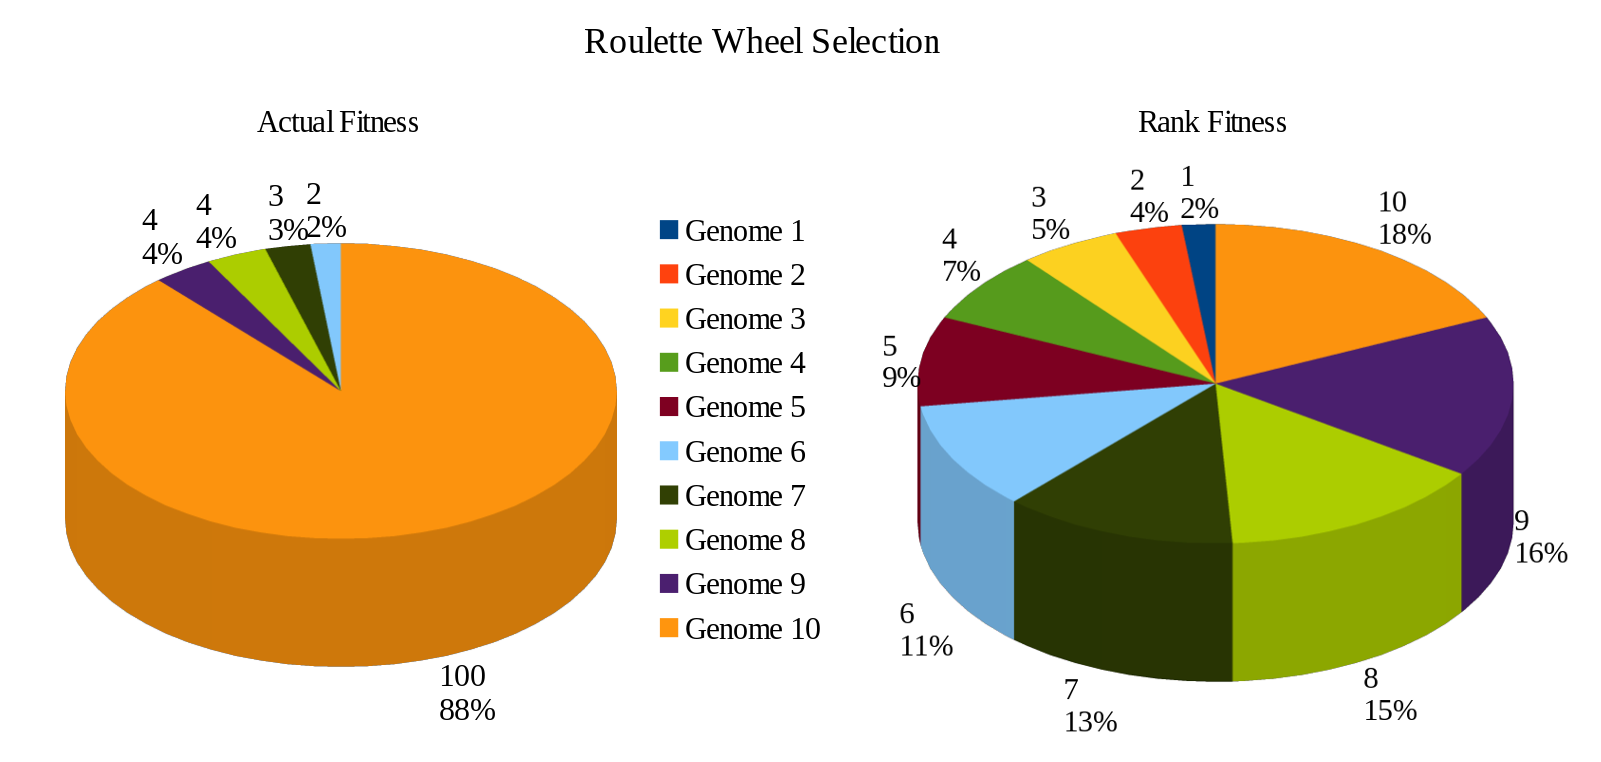
\includegraphics[scale=0.25]{../Figures/Chapter3/roulette.png}
  \rule{35em}{0.5pt}
  \caption[Roulette Wheel Selection]{Here you see roulette selection using actual fitness versus rank fitness for a population of 10 genomes. On the left, the integers are the genomes' actual fitness and the percentages are their probabilities of being selected. On the right, the integers are the genomes' rank fitness and the percentages are the genomes' probabilities of being selected. Observe that Genome 10 no longer dominates the wheel when using its rank fitness ($10$) versus using its actual fitness ($100)$.}
  \label{fig:roulette}
\end{figure}

Crossover probability was increased from $0.7$ to $0.8$. This of course would result in more observed crossovers being generated as new populations were created. Since crossover produces an offspring solution  somewhere between its parents in the fitness landscape, it was hypothesized that by increasing the crossover probability the local search capability of the genetic algorithm would also increase.

Based on empirical studies performed by others, setting the mutation probability to $\frac{1}{n}$---where $n$ is the number of genes per genome---is a sufficient enough amount of random search to allow the genetic algorithm to escape local maxima in the fitness landscape \cite{predictive_models}. The reasoning behind $\frac{1}{n}$ is that per mutation on a gene-by-gene basis, only one gene is mutated on average. In addition to changing the mutation probability, the mutation step was changed from adding and/or subtracting a percentage of a maximum perturbation parameter value to and/or from the gene value to sampling a value from a Gaussian distribution where the distribution $N(\mu,\sigma^2)$ is defined by the mean $\mu$ being the gene's current value before mutation and the standard deviation $\sigma$ being one fourth the valid range of the gene/parameter $\left(\frac{1-(-1)}{4}=0.5 \right)$. Here the standard deviation $\sigma$ is one fourth the range and thus most of the sampled values will be within two standard deviations of the mean $\mu$ or rather the gene value. Any sampled gene value that was outside the valid range of $[-1,1]$ was clipped to the valid range. Note that by going with this new mutation step schema, the maximum perturbation parameter to the genetic algorithm could be removed thereby lessening the amount of parameters---to the genetic algorithm---that need to be evaluated. 

\begin{table}[htbp]
\centering
\footnotesize
\begin{tabular}{ | >{\columncolor[gray]{0.8}} m{5cm}  || >{\centering\arraybackslash}m{5cm} | }
\hline
Population Size                                                      & 10                                                                \\ \hline
Number of Elite Offspring                                            & 2                                                                 \\ \hline
Roulette Selection using Actual Fitness                              & False                                                             \\ \hline
Roulette Selection using Rank Fitness                                & True                                                              \\ \hline
Crossover Probability                                                & 0.8                                                               \\ \hline
Crossover Type                                                       & One Point Crossover                                               \\ \hline
Mutation Probability                                                 & $\frac{1}{n \ genes}=\frac{1}{41} = 0.024390244$                  \\ \hline
Mutation Scope                                                       & Gene Level                                                        \\ \hline
Mutation Step                                                        & $X\sim N(\mu,\sigma^2)$                                           \\ \hline
Mutation Step $\mu$                                                  & Gene Value                                                        \\ \hline
Mutation Step $\sigma$                                               & $0.5$                                                             \\ \hline
Max Perturbation                                                     & N/A                                                       	       \\ \hline
Sequential Crossover and Mutation                                    & True                                                      	       \\ \hline
%Offspring not Crossed/Mutated Allowed in New Generation             & True                                                     	       \\ \hline
Fitness Function                                                     & Full                                                              \\ \hline
Fitness Credit for Staying in the Path of the Ball                   & 1.0                                                      	       \\ \hline
Fitness Credit for not Staying in the Path of the Ball               & 0.0                                                      	       \\ \hline
\end{tabular}
\caption[Experiment Two GA Parameters]{Here you see the genetic algorithm parameters for experiment two.}
\label{tab:exp2}
\end{table}

\subsection[Experiment Three]{Experiment three: self-adaptation of crossover and mutation probabilities with the crossover and mutation operators working in parallel.}

Experiment three involved self-adaptation of the crossover and mutation probabilities. The genetic algorithm parameters used are listed in Table \ref{tab:exp3}.

As outlined in \cite{self_adapt}, the crossover and mutation probabilities self-adapt based on the crossover and mutation operators' ability to produce fitter genomes from one generation to the next. To facilitate the self-adaptation, the crossover and mutation operators' viability to produce fitter and fitter offspring needed to be tracked from one generation to another. As the operators were being evaluated on their own accord, they were not allowed to interfere with each others' offspring and thus they were not run in sequence but rather were run in parallel. With each new generation produced, elite offspring were marked accordingly as well as offspring produced by crossover and offspring produced by mutation. For those offspring that were created by crossover, their parents' weighted-mean fitness was annotated along with their offspring. Annotated meaning it was recorded in the offspring's data structure later being used to calculate the crossover operator's progress. This weighted-mean fitness was calculated based on the crossover point which determines what percentage of genes came come from parent one and what percentage of genes came from parent two. For example, let there be 41 genes per genome and let the crossover point be gene 10. Thus, offspring one received 10 genes from parent one and received 31 genes from parent two while offspring two received 10 genes from parent two and received 31 genes from parent one. Therefore, offspring one's weighted-mean parent fitness would be calculated as $\overline{PF} = \left ( PF_1 * \frac{10}{41} \right ) + \left (PF_2 * \frac{(41-10)}{41} \right)$ where $\overline{PF}$ is the weighted-mean parent fitness while offspring two's weighted-mean parent fitness would be calculated as $\overline{PF} = \left ( PF_2 * \frac{10}{41} \right ) + \left (PF_1 * \frac{(41-10)}{41} \right)$. For those offspring created via mutation, their parent fitness was whatever the fitness was of the pre-mutated genome. 

With the genomes marked as to how they were created and their parent fitness annotated, now when it came time to produce a new population, each operators' ability to produce fitter offspring could be tracked and calculated. Once a population was evaluated, all genomes created by crossover were used to calculate the average crossover progress and all genomes created by mutation were used to calculate the average mutation progress. If the crossover progress average was greater than the mutation progress average then the crossover probability would be adjusted up and the mutation probability would be adjusted down. Alternatively, if the crossover progress average was less than the mutation progress average then the crossover probability would be adjusted down and the mutation probability would be adjusted up. If the crossover progress average equaled the mutation progress average then neither were adjusted. In other words, for example, if the crossover operator produced fitter genomes greater than the mutation operator did for the last generation, then the probability of creating offspring via crossover would be increased and the probability of creating offspring via mutation would be decreased for the creation of the next generation. Adjustment of the crossover and mutation probabilities were handled by the adjustment parameter. Let the adjustment parameter be denoted as $\theta$. Here $\theta$ was self-adjusted as well, as outlined in \cite{self_adapt}. Once the probabilities were adjusted they were clamped to the range $[0.001,1.0]$. With a minimum probability of $0.001$, there would always be some crossover and/or mutation albeit not much. See Figure \ref{fig:sa}. Note that to insure a level playing field, both the crossover and mutation probabilities were set to an initial value of $0.5$ before the start of the genetic algorithm.

\renewcommand{\baselinestretch}{1.0}

\begin{figure}[htbp]
\begin{center}
\begin{varwidth}{\textwidth}
{\tt
BEGIN \\
\tab Population $P$ has been evaluated \\
\tab $cCount = mCount = 0$ \\
\tab $CP_{sum} = MP_{sum} = 0$ \\
\tab $\overline{CP} = \overline{MP} = 0$ \\
\tab For $j=1$ to population size do \\
\tab \tab If $P[j]$ created by crossover then \\
\tab \tab \tab $CP_{sum} = CP_{sum} + (P[j].fitness - P[j].parentFitness)$ \\
\tab \tab \tab $cCount = cCount + 1$\\
\tab \tab Else if $P[j]$ created by mutation then\\
\tab \tab \tab $MP_{sum} = MP_{sum} + (P[j].fitness - P[j].parentFitness)$ \\
\tab \tab \tab $mCount = mCount + 1$ \\
\tab \tab End if \\
\tab End for \\
\tab $\overline{CP} = \frac{CP_{sum}}{cCount}$ \\
\tab $\overline{MP} = \frac{MP_{sum}}{mCount}$ \\
\tab If $P.bestFitness$ $>$ $P.worstFitness$ then \\
\tab \tab Adjustment $\theta = 0.01 * \frac{P.bestFitness - P.meanFitness}{P.bestFitness - P.worstFitness}$ \\
\tab Else if $P.bestFitness$ $=$ $P.meanFitness$ then \\
\tab \tab Adjustment $\theta = 0.01$ \\
\tab End if \\
\tab If $\overline{CP} > \overline{MP}$ then \\
\tab \tab Crossover Probability $C = C + \theta$ \\
\tab \tab Mutation Probability $M = M - \theta$ \\
\tab Else if $\overline{CP} < \overline{MP}$ then \\
\tab \tab Crossover Probability $C = C - \theta$ \\
\tab \tab Mutation Probability $M = M + \theta$ \\
\tab End if \\
\tab Clamp C to range $[0.001,1.0]$ \\
\tab Clamp M to range $[0.001,1.0]$ \\
END \\
}
% \begin{equation*}
% \boxed{
% \begin{aligned}
% Begin: &  \\
% & Population \ P_i \ has \ been \ evaluated. \\
% & cCount = mCount = 0. \\
% & CP_{sum} = MP_{sum} = 0. \\
% & \overline{CP} = \overline{MP} = 0. \\
% & For \ j = 1 \ to \ population \ size: \\
% & \quad If \ genome_j \ created \ by \ crossover: \\
% & \quad\quad\quad CP_{sum} \longleftarrow CP_{sum} + ( genome_j.fitness - genome_j.parentFitness ). \\
% & \quad\quad\quad cCount \longleftarrow cCount + 1. \\
% & \quad Else \ if \ genome_j \ created \ by \ mutation: \\
% & \quad\quad\quad MP_{sum} \longleftarrow MP_{sum} + (genome_j.fitness - genome_j.parentFitness). \\
% & \quad\quad\quad mCount \longleftarrow mCount + 1. \\
% & \overline{CP} = \frac{CP_{sum}}{cCount}. \\
% & \overline{MP} = \frac{MP_{sum}}{mCount}. \\
% & If \ P_i \ Best \ Fitness > P_i \ Worst \ Fitness: \\
% & \quad \theta \longleftarrow 0.01 * \frac{P_i \ Best \ Fitness - P_i \ Mean \ Fitness }{P_i \ Best \ Fitness - P_i \ Worst \ Fitness }.\\
% & Else  \ if \ P_i \ Best \ Fitness = P_i \ Mean \ Fitness: \\
% & \quad \theta \longleftarrow 0.01  \ . \\
% & If \ \overline{CP} > \overline{MP}: \\
% & \quad Crossover \ Prob. \longleftarrow Crossover \ Prob. + \theta. \\
% & \quad Mutation \ Prob. \longleftarrow Mutation \ Prob. - \theta. \\
% & Else \ if \ \overline{CP} < \overline{MP}: \\
% & \quad Crossover \ Prob. \longleftarrow Crossover \ Prob. - \theta. \\
% & \quad Mutation \ Prob. \longleftarrow Mutation \ Prob. + \theta. \\
% & Clamp \ Crossover \ Prob. \ to \ [0.001, 1.0]. \\
% & Clamp \ Mutation \ Prob. \ to \ \ [0.001, 1.0]. \\
% \end{aligned}
% }
% \end{equation*}
\end{varwidth}
\end{center}
\centering
\rule{35em}{0.5pt}
\caption[Self-adaptation Algorithm]{Here you see the self-adaptation algorithm.}
\label{fig:sa}
\end{figure}

\vspace{3mm}

Unlike previous experiments, the mutation probability was not set on a gene-by-gene basis but rather on a whole genome-by-genome basis. Every time through the population creation loop, a random float value was sampled from a uniform distribution between $0.0$ and $1.0$. If this random float value was less than or equal to the mutation probability, every gene in the selected genome was mutated using the Gaussian distribution mutation step method outlined earlier. However, the standard deviation was set to the mutation probability instead of it being statically set to $0.5$ as before. The reason being that a high mutation probability would give way to a larger mutation step (since the standard deviation would be relatively large) allowing for larger random leaps around the fitness landscape while a low mutation probability would give way to a smaller mutation step (since the standard deviation would be relatively small) allowing for a more finely tuned search as the population converges to the optimum in the fitness landscape.

\begin{table}[htbp]
\centering
\footnotesize
\begin{tabular}{ | >{\columncolor[gray]{0.8}} m{5cm}  || >{\centering\arraybackslash}m{5cm} | }
\hline
Population Size                                                      & 10                                                                           \\ \hline
Number of Elite Offspring                                            & 2                                                                            \\ \hline
Roulette Selection using Actual Fitness                              & False                                                                        \\ \hline
Roulette Selection using Rank Fitness                                & True                                                                         \\ \hline
Self-adaptation                                                      & True                                                                         \\ \hline
Initial Crossover Probability                                        & 0.5                                                                          \\ \hline
Minimum Crossover Probability                                        & 0.001                                                                        \\ \hline
Crossover Type                                                       & One Point Crossover                                                          \\ \hline
Initial Mutation Probability                                         & 0.5                                                                          \\ \hline
Minimum Mutation Probability                                         & 0.001                                                                        \\ \hline
Mutation Scope                                                       & Genome Level                                                                 \\ \hline
Mutation Step                                                        & $X\sim N(\mu,\sigma^2)$                                                      \\ \hline
Mutation Step $\mu$                                                  & Gene Value                                                                   \\ \hline
Mutation Step $\sigma$                                               & Mutation Probability                                                         \\ \hline
Sequential Crossover and Mutation                                    & False                                                      	\\ \hline
%Offspring not Crossed/Mutated Allowed in New Generation             & False                                                    	\\ \hline
Fitness Function                                                     & Full                                                                         \\ \hline
Fitness Credit for Staying in the Path of the Ball                   & 1.0                                                      	\\ \hline
Fitness Credit for not Staying in the Path of the Ball               & 0.0                                                      	\\ \hline
\end{tabular}
\caption[Experiment Three GA parameters]{Here you see the genetic algorithm parameters for experiment three.}
\label{tab:exp3}
\end{table}

\subsection[Experiment Four]{Experiment four: static crossover and mutation probabilities with the crossover and mutation operators working in parallel.}

Experiment four had an identical setup to experiment three with the exception that the crossover and mutation probabilities were statically set, throughout the experiment, to the crossover and mutation probabilities arrived at after the 100th generation of the genetic algorithm in experiment three. The genetic algorithm parameters used are listed in Table \ref{tab:exp4}.

Experiment four as well as experiment five were devised as comparisons to experiment three. The hypothesis was that self-adaptation, along with non-interfering operators, would have the fastest average fitness growth rate among the three.

\begin{table}[htbp]
\centering
\footnotesize
\begin{tabular}{ | >{\columncolor[gray]{0.8}} m{5cm}  || >{\centering\arraybackslash}m{5cm} | }
\hline
Population Size                                                      & 10                                                                           \\ \hline
Number of Elite Offspring                                            & 2                                                                            \\ \hline
Roulette Selection using Actual Fitness                              & False                                                                        \\ \hline
Roulette Selection using Rank Fitness                                & True                                                                         \\ \hline
Self-adaptation                                                      & False                                                                        \\ \hline
Crossover Probability                                                & 0.7816                                                                       \\ \hline
Crossover Type                                                       & One Point Crossover                                                          \\ \hline
Mutation Probability                                                 & 0.2184                                                                       \\ \hline
Mutation Scope                                                       & Genome Level                                                                 \\ \hline
Mutation Step                                                        & $X\sim N(\mu,\sigma^2)$                                                      \\ \hline
Mutation Step $\mu$                                                  & Gene Value                                                                   \\ \hline
Mutation Step $\sigma$                                               & Mutation Probability                                                         \\ \hline
Sequential Crossover and Mutation                                    & False                                                      	             \\ \hline
%Offspring not Crossed/Mutated Allowed in New Generation             & False                                                   	                  \\ \hline
Fitness Function                                                     & Full                                                                         \\ \hline
Fitness Credit for Staying in the Path of the Ball                   & 1.0                                                      	                  \\ \hline
Fitness Credit for not Staying in the Path of the Ball               & 0.0                                                      	                  \\ \hline
\end{tabular}
\caption[Experiment Four GA Parameters]{Here you see the genetic algorithm parameters for experiment four.}
\label{tab:exp4}
\end{table}

\subsection[Experiment Five]{Experiment five: static crossover and mutation probabilities with the crossover and mutation operators working in sequence.}

Experiment five had an identical setup as experiment four with the exception that the crossover and mutation operators were run in sequence instead of in parallel. By running the operators in sequence, the mutation operator could disrupt the offspring created by the crossover operator. The genetic algorithm parameters used are listed in Table \ref{tab:exp5}.

%Experiment five as well as experiment four were devised as comparisons to experiment three. The hypothesis was that self-adaptation, along with non-interfering operators, would have the fastest average fitness growth rate among the three.

\begin{table}[htbp]
\centering
\footnotesize
\begin{tabular}{ | >{\columncolor[gray]{0.8}} m{5cm}  || >{\centering\arraybackslash}m{5cm} | }
\hline
Population Size                                                      & 10                                                                             \\ \hline
Number of Elite Offspring                                            & 2                                                                              \\ \hline
Roulette Selection using Actual Fitness                              & False                                                                          \\ \hline
Roulette Selection using Rank Fitness                                & True                                                                           \\ \hline
Self-adaptation                                                      & False                                                                          \\ \hline
Crossover Probability                                                & 0.7816                                                                         \\ \hline
Crossover Type                                                       & One Point Crossover                                                            \\ \hline
Mutation Probability                                                 & 0.2184                                                                         \\ \hline
Mutation Scope                                                       & Gene Level                                                                     \\ \hline
Mutation Step                                                        & $X\sim N(\mu,\sigma^2)$                                                        \\ \hline
Mutation Step $\mu$                                                  & Gene Value                                                                     \\ \hline
Mutation Step $\sigma$                                               & Mutation Probability                                                           \\ \hline
Sequential Crossover and Mutation                                    & True                                                      	                    \\ \hline
%Offspring not Crossed/Mutated Allowed in New Generation             & False                                                      	               \\ \hline
Fitness Function                                                     & Full                                                                           \\ \hline
Fitness Credit for Staying in the Path of the Ball                   & 1.0                                                      	                    \\ \hline
Fitness Credit for not Staying in the Path of the Ball               & 0.0                                                      	                    \\ \hline
\end{tabular}
\caption[Experiment Five GA Parameters]{Here you see the genetic algorithm parameters for experiment five.}
\label{tab:exp5}
\end{table}

\subsection[Experiment Six]{Experiment Six: fitness and ball-in-play upper bound.}

The setup for experiment six was identical to that of experiment two, three, four, and five with the exception that no evolution ever took place (crossover and mutation probabilities were set to $0.0$) during the run of the genetic algorithm over 100 generations. Only the simplified fitness function (described in experiment two) was used during the run of the genetic algorithm. With no evolution taking place, the number-of-elite-offspring parameter was set to $10$---equal to the population size---in order to use the same genetic algorithm code base that was implemented and employed for the previous experiments. The genetic algorithm parameters used are listed in Table \ref{tab:exp6}. 

The goal of experiment six was to obtain the average fitness over 100 generations, the fitness of every 10th generation top performer, and the average ball-in-play time of five rounds per every 10th generation top performer \textbf{where the paddle always performed the correct movement} no matter the state of the paddle and the ball at any time during any round. In other words, the goal of experiment six was to obtain an average fitness upper bound and an average ball-in-play time of five rounds upper bound utilizing the same fitness function as was used in experiment two, three, four, and five. 

To accomplish the goal of experiment six, the neural-network output was ignored and instead, the paddle's center height (y-coordinate) was always set to the ball's center y-coordinate once every draw loop. With this modification, the paddle was always dead center with the ball, was always in the path of the ball, and thus always kept the ball from leaving the left side of the arena. That is, it always hit the ball back into the arena. At no point was the paddle ever not in the path of the ball and thus the paddle always obtained the maximum fitness possible as well as the maximum ball-in-play time possible for any particular round. The only way any round ever terminated was by the ball's velocity magnitude falling below the $100$ threshold.  

% the difference in heights between the paddle's center and the ball's center was used to determine the paddle's velocity magnitude and its velocity angle at every draw loop. If the difference was $\vartriangle\!y<0$ (meaning the paddle was higher up the screen than the ball) the paddle's velocity angle was set to $\theta=270.0^\circ$ and the paddle's velocity magnitude was set to $m = -1 * \vartriangle\!y * 10$. Otherwise, if the difference was $\vartriangle\!y\geq 0$ (meaning the paddle was lower down the screen than the ball) the paddle's velocity angle was set to $\theta=90.0^\circ$ and the paddle's velocity magnitude was set to $m = \vartriangle\!y * 10$. With this modification, the paddle was always in the path of the ball and thus always kept the ball from leaving the left side of the arena. That is, it always hit the ball back into the arena. At no point was the paddle ever not in the path of the ball and thus the paddle always obtained the maximum fitness possible as well as the maximum ball-in-play time possible for any particular round. The only way any round ever terminated was by the ball's velocity magnitude falling below the $100$ threshold. 

\begin{table}[htbp]
\centering
\footnotesize
\begin{tabular}{ | >{\columncolor[gray]{0.8}} m{5cm}  || >{\centering\arraybackslash}m{5cm} | }
\hline
Population Size                                                      & 10                                                                       \\ \hline
Number of Elite Offspring                                            & 10                                                                       \\ \hline
Roulette Selection using Actual Fitness                              & N/A                                                                      \\ \hline
Roulette Selection using Rank Fitness                                & N/A                                                                      \\ \hline
Self-adaptation                                                      & N/A                                                                      \\ \hline
Crossover Probability                                                & N/A                                                                      \\ \hline
Crossover Type                                                       & N/A                                                                      \\ \hline
Mutation Probability                                                 & N/A                                                                      \\ \hline
Mutation Scope                                                       & N/A                                                                      \\ \hline
Mutation Step                                                        & N/A                                                                      \\ \hline
Sequential Crossover and Mutation                                    & N/A                                                       	\\ \hline
%Offspring not Crossed/Mutated Allowed in New Generation             & N/A                                                      	\\ \hline
Fitness Function                                                     & Full                                                                     \\ \hline
Fitness Credit for Staying in the Path of the Ball                   & 1.0                                                      	\\ \hline
Fitness Credit for not Staying in the Path of the Ball               & 0.0                                                      	\\ \hline
\end{tabular}
\caption[Experiment Six GA Parameters]{Here you see the genetic algorithm parameters for experiment six.}
\label{tab:exp6}
\end{table}

\subsection[Experiment Seven]{Experiment seven: random paddles.} 

% So how the random paddle was created using pseudo-code. Talk about how this experiment was done to show that the GA genomes/NNs/paddles perform better than random.

The setup for experiment seven was identical to that of experiment six where no evolution ever took place (crossover and mutation probabilities were set to $0.0$) during the run of the genetic algorithm over 100 generations. Only the simplified fitness function (described in experiment two) was used during the run of the genetic algorithm. With no evolution taking place, the number-of-elite-offspring parameter was set to $10$---equal to the population size---in order to use the same genetic algorithm code base that was implemented and employed for the previous experiments. The genetic algorithm parameters used are listed in Table \ref{tab:exp7}. 

The goal of experiment seven was to obtain the average fitness over 100 generations, the fitness of every 10th generation top performer, and the average ball-in-play time of five rounds per every 10th generation top performer \textbf{where the paddle always performed a random movement}. By obtaining these metrics for randomly moving paddles, it could be demonstrated that the genetic algorithm either did or did not ultimately produce paddles that performed better than the randomly moving paddles. 

To accomplish the goal of experiment seven, the neural-network output was ignored and instead, the paddle's movement was always randomly generated once per draw loop. To generate the random movement, a random float was sampled from a uniform distribution $X\sim U(-1,1)$. If $X$ was in the range $[-1,0)$, the paddle's velocity angle was set to $270^\circ$ and the paddle's velocity magnitude was set to $m_{new} = -1 * X * m_{initial}$ where $m_{initial}$ was the paddle's starting velocity magnitude (specifically $1000 \ \frac{pixels}{second}$). If $X$ was in the range $(0,1]$, the paddle's velocity angle was set to $90^\circ$ and the paddle's velocity magnitude was set to $m_{new} = X * m_{initial}$. Otherwise, if $X$ was zero, the paddle did not move from its current position. 

\begin{table}[htbp]
\centering
\footnotesize
\begin{tabular}{ | >{\columncolor[gray]{0.8}} m{5cm}  || >{\centering\arraybackslash}m{5cm} | }
\hline
Population Size                                                      & 10                                                                       \\ \hline
Number of Elite Offspring                                            & 10                                                                       \\ \hline
Roulette Selection using Actual Fitness                              & N/A                                                                      \\ \hline
Roulette Selection using Rank Fitness                                & N/A                                                                      \\ \hline
Self-adaptation                                                      & N/A                                                                      \\ \hline
Crossover Probability                                                & N/A                                                                      \\ \hline
Crossover Type                                                       & N/A                                                                      \\ \hline
Mutation Probability                                                 & N/A                                                                      \\ \hline
Mutation Scope                                                       & N/A                                                                      \\ \hline
Mutation Step                                                        & N/A                                                                      \\ \hline
Sequential Crossover and Mutation                                    & N/A                                                       	\\ \hline
%Offspring not Crossed/Mutated Allowed in New Generation             & N/A                                                      	\\ \hline
Fitness Function                                                     & Full                                                                     \\ \hline
Fitness Credit for Staying in the Path of the Ball                   & 1.0                                                      	\\ \hline
Fitness Credit for not Staying in the Path of the Ball               & 0.0
\\ \hline
\end{tabular}
\caption[Experiment Seven GA Parameters]{Here you see the genetic algorithm parameters for experiment seven.}
\label{tab:exp7}
\end{table}

\section{Experimental Results}

The results of each experiment are presented below (Sections 5.1 through 5.7), followed by a comparison of all results (Section 5.8).

For each experiment (one through seven), there are three plots shown. The first plot shows the average fitness over 100 generations. The second plot shows the fitness of the top performer for every 10th generation (over 100 generations). The third plot shows the ball-in-play time, averaged over 5 games, for the top performers whose fitness is illustrated in the second plots.

\subsection[Experiment One]{Experiment one: use of a full and partial credit granting fitness function.}

Experiment one (Figures \ref{fig:exp1_avg_fit}-\ref{fig:exp1_10_tops_times}) show that the player learns to keep the ball in play longer after generation 49, improving from 3.00584 seconds per round on average to 28.30964 seconds. This is despite the fact that the average fitness doesn't begin to show significant improvement until generation 80. Indeed, it is strange that the improvement in average ball-in-play time drops in generation 79, but then improves and exceeds the previous maximum (generation 69) after generation 89.

\begin{figure}[htbp]  
  \centering
  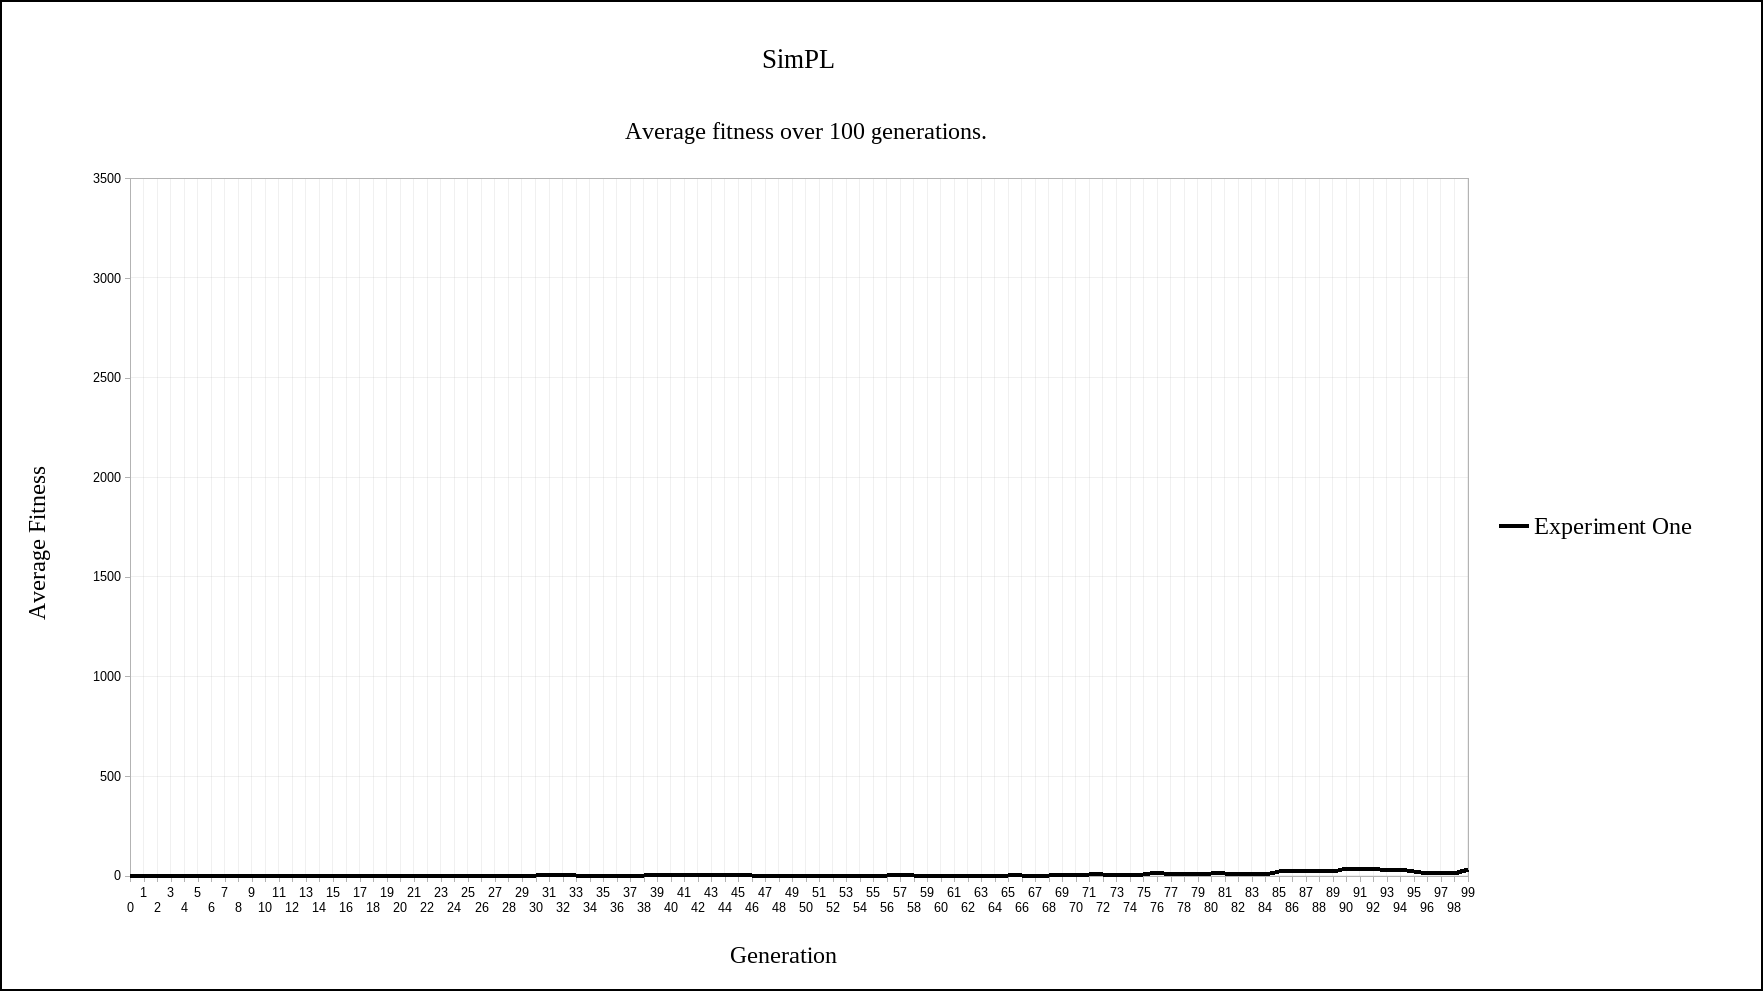
\includegraphics[width=5in]{../Figures/Chapter3/exp1_avg_fit.png}
  \rule{35em}{0.5pt}
  \caption[Experiment One Average Fitness]{Here you see the average fitness over 100 generations for experiment one.}
  \label{fig:exp1_avg_fit}
\end{figure}

\begin{figure}[htbp]  
  \centering
  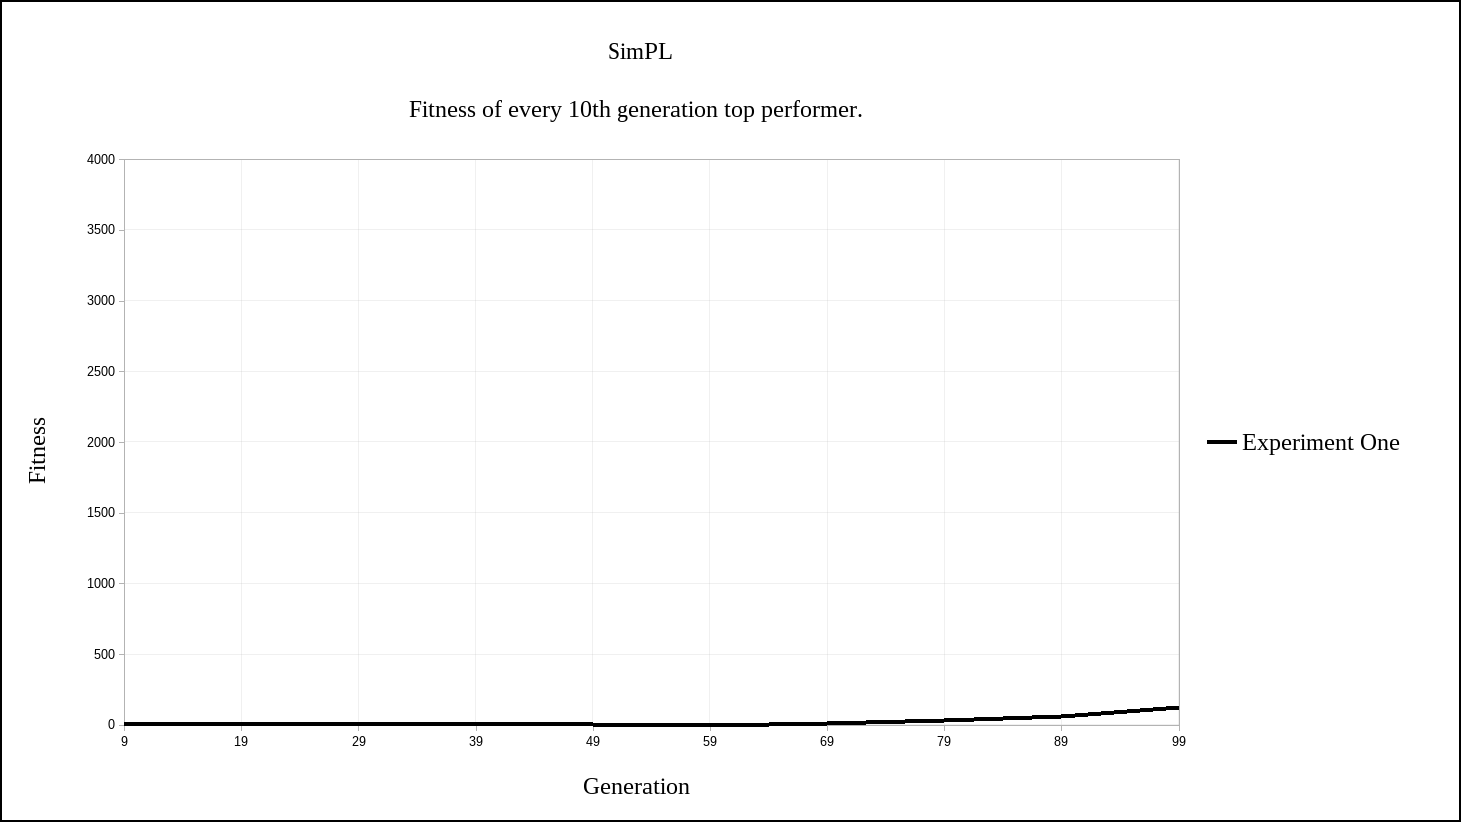
\includegraphics[width=5in]{../Figures/Chapter3/exp1_10_tops.png}
  \rule{35em}{0.5pt}
  \caption[Experiment One Top Performers]{Here you see the fitness of every 10th generation top performer for experiment one.}
  \label{fig:exp1_10_tops}
\end{figure}

\begin{figure}[htbp]  
  \centering
  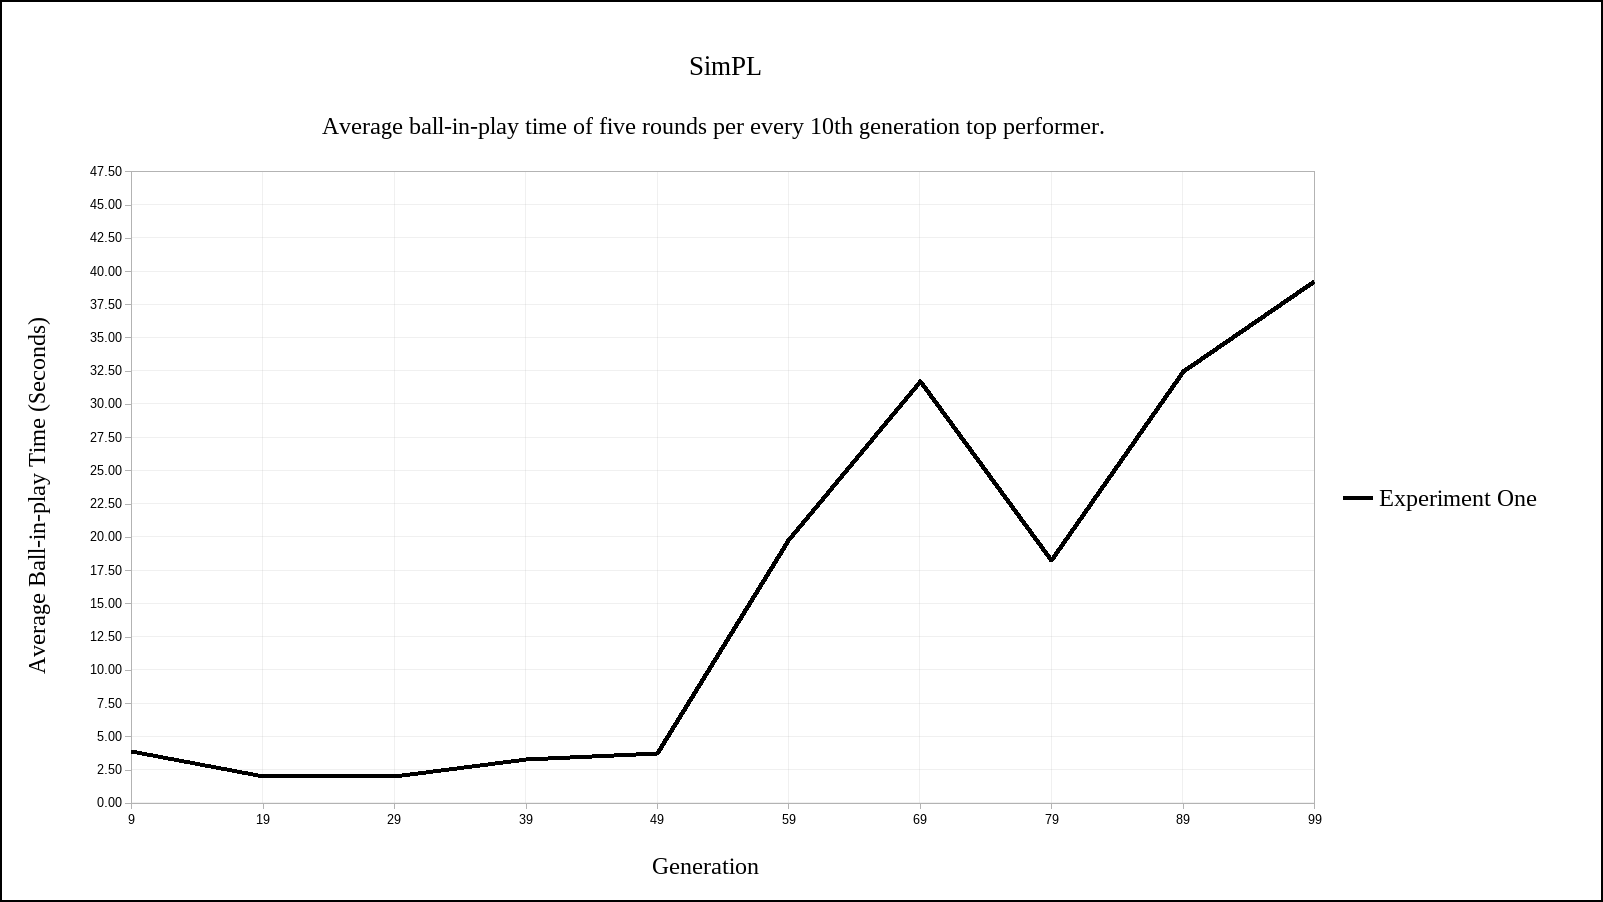
\includegraphics[width=5in]{../Figures/Chapter3/exp1_10_tops_times.png}
  \rule{35em}{0.5pt}
  \caption[Experiment One Top Performers Tournament]{Here you see the average ball-in-play time (in seconds) of five rounds per every 10th generation top performer for experiment one.}
  \label{fig:exp1_10_tops_times}
\end{figure}

\subsection[Experiment Two]{Experiment two: use of a simplified fitness function, use of rank fitness in selection, higher crossover probability, mutation probability based on the number of genes per genome, and a Gaussian distribution sample mutation step.}

Experiment two (Figures \ref{fig:exp2_avg_fit}-\ref{fig:exp2_10_tops_times}) shows marked improvement in average fitness to generation 20, and then a more gradual improvement for the remaining 80 generations. The average ball-in-play times improve dramatically from 10.1 seconds to 37.8 seconds within the first 20 generations, but levels off and does not show marked improvement for the remainder of the experiment.

\begin{figure}[htbp]  
  \centering
  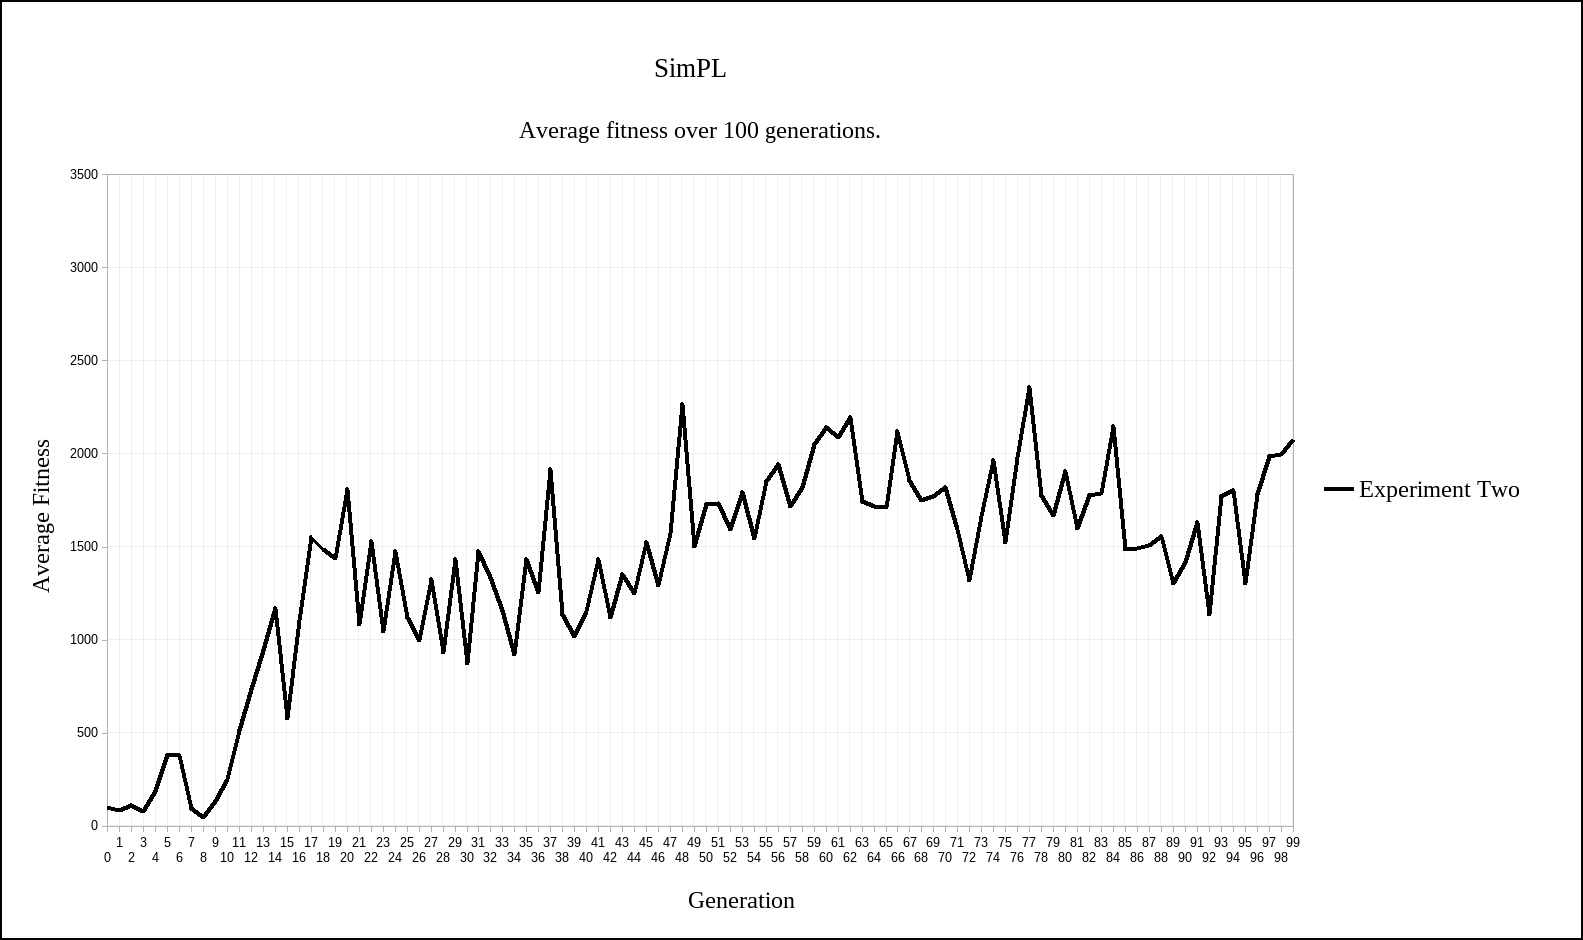
\includegraphics[width=5in]{../Figures/Chapter3/exp2_avg_fit.png}
  \rule{35em}{0.5pt}
  \caption[Experiment Two Average Fitness]{Here you see the average fitness over 100 generations for experiment two.}
  \label{fig:exp2_avg_fit}
\end{figure}

\begin{figure}[htbp]  
  \centering
  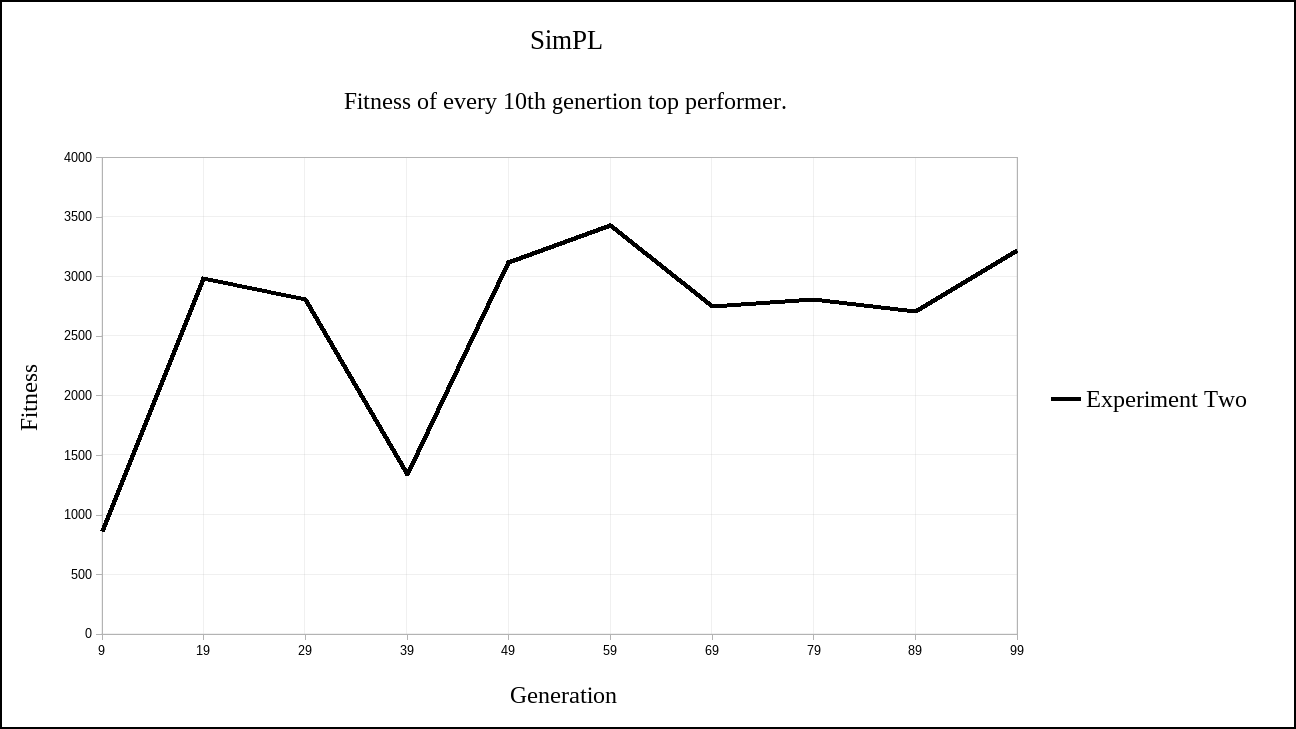
\includegraphics[width=5in]{../Figures/Chapter3/exp2_10_tops.png}
  \rule{35em}{0.5pt}
  \caption[Experiment Two Top Performers]{Here you see the fitness of every 10th generation top performer for experiment two.}
  \label{fig:exp2_10_tops}
\end{figure}

\begin{figure}[htbp]  
  \centering
  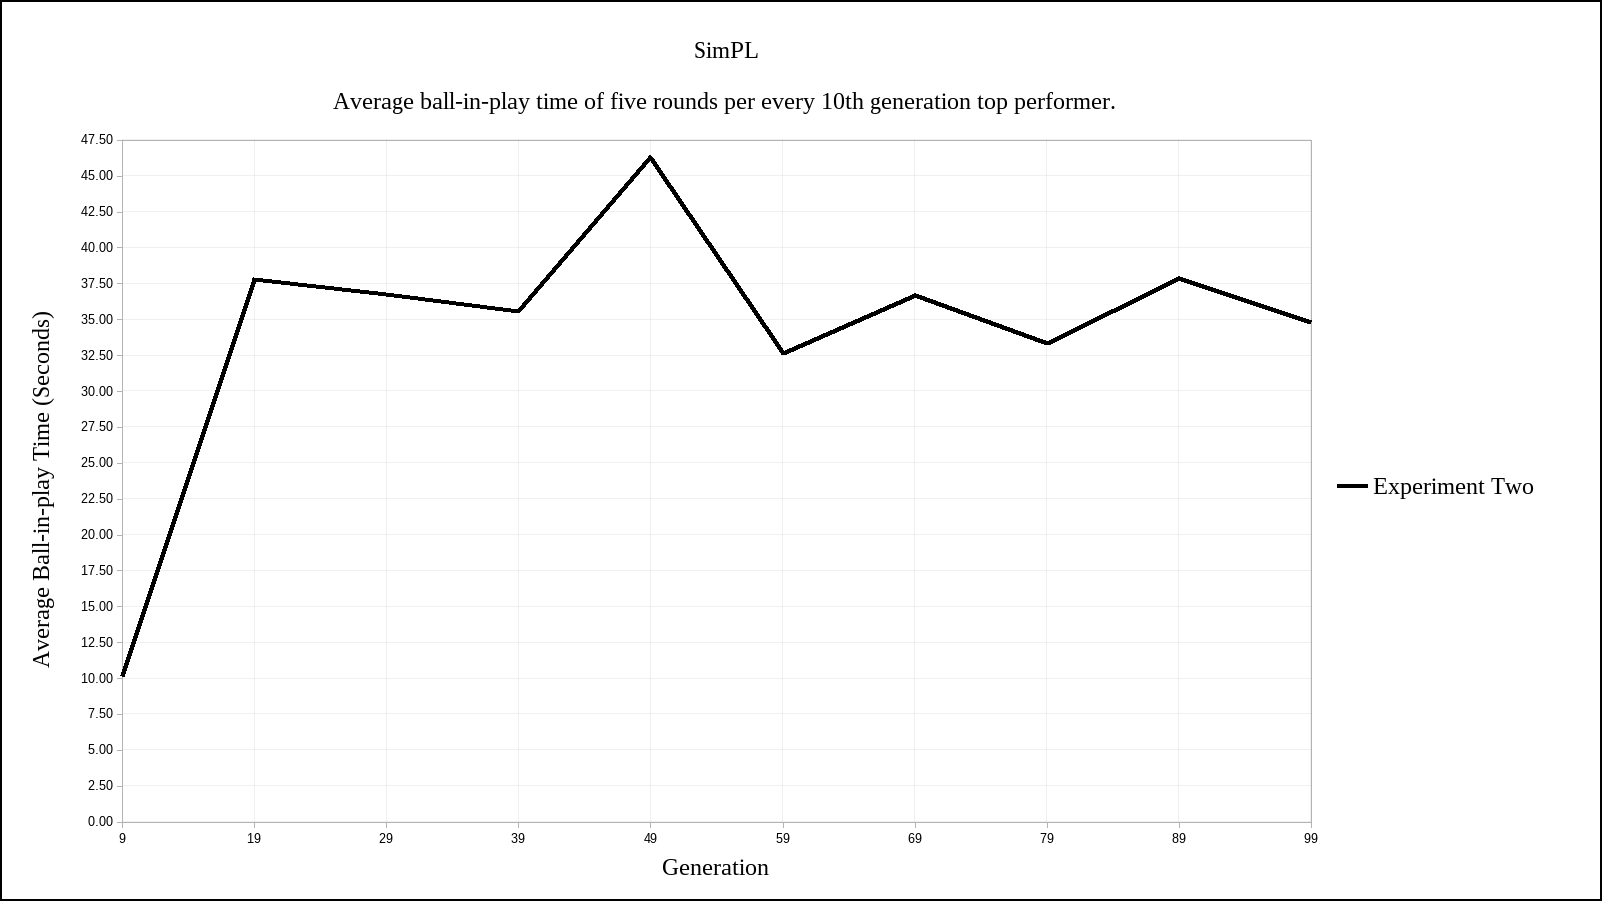
\includegraphics[width=5in]{../Figures/Chapter3/exp2_10_tops_times.png}
  \rule{35em}{0.5pt}
  \caption[Experiment Two Top Performers Tournament]{Here you see the average ball-in-play time (in seconds) of five rounds per every 10th generation top performer for experiment two.}
  \label{fig:exp2_10_tops_times}
\end{figure}

\subsection[Experiment Three]{Experiment three: self-adaptation of crossover and mutation probabilities with the crossover and mutation operators working in parallel.}

Experiment three (Figures \ref{fig:exp3_avg_fit}-\ref{fig:exp3_10_tops_times}) shows initial improvement in average fitness for the first 12 generations, but then oscillates and does not show measurable improvement for the rest of the experiment. This result is reflected in the average ball-in-play time metric, which starts at 35.7314 seconds and oscillates but does not trend significantly. Figure \ref{fig:exp3_self_adapt} illustrates the self-adaptation of the crossover and mutation probabilities, as chosen by the algorithm at run-time. Although the proportions change, they do not appear to correlate with the fitness or average ball-in-play time results.

\begin{figure}[htbp]  
  \centering
  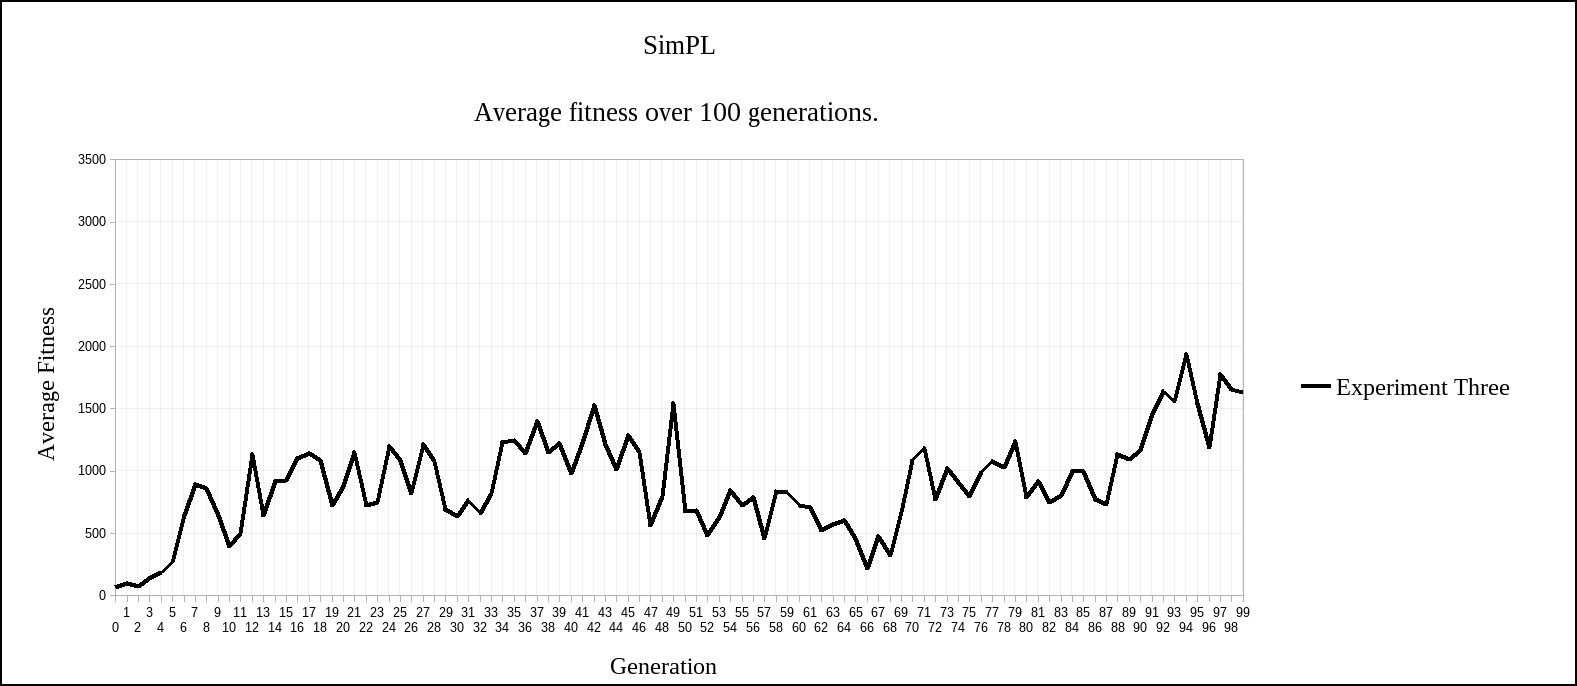
\includegraphics[width=5in]{../Figures/Chapter3/exp3_avg_fit.png}
  \rule{35em}{0.5pt}
  \caption[Experiment Three Average Fitness]{Here you see the average fitness over 100 generations for experiment three.}
  \label{fig:exp3_avg_fit}
\end{figure}

The crossover and mutation probabilities were both initially set to $0.5$ before the start of the experiment. After the experiment was over, the genetic algorithm self-adapted the crossover probability to $0.7816$ and self-adapted the mutation probability to $0.2184$. You'll notice in Figure \ref{fig:exp3_self_adapt} that the mutation probability overtook the crossover probability at first but the two probabilities eventually diverged with mutation becoming less probable and crossover becoming more probable as the genetic algorithm produced fitter generations. This outcome is almost the exact opposite of the outcome shown in \cite{self_adapt}.

\begin{figure}[htbp]  
  \centering
  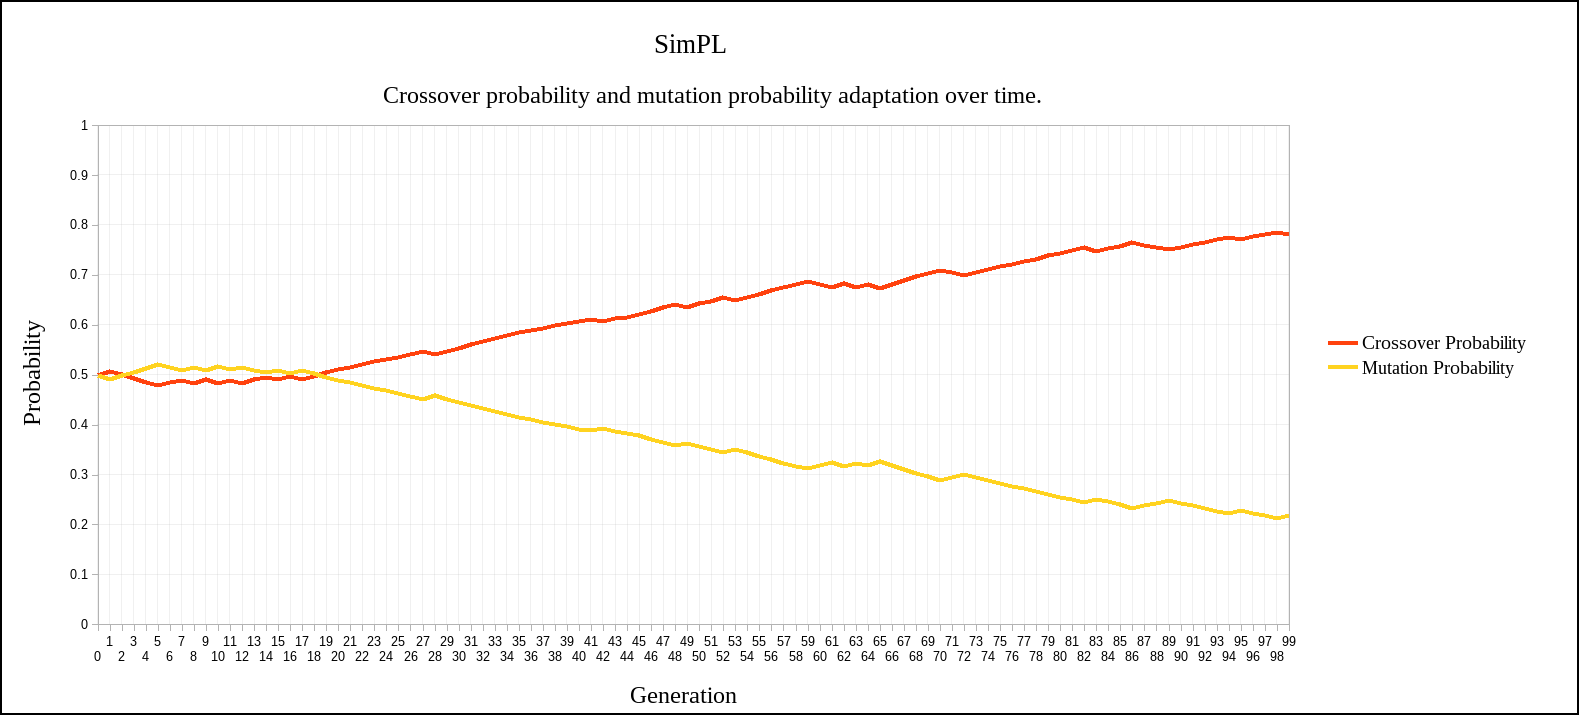
\includegraphics[width=5in]{../Figures/Chapter3/exp3_self_adapt.png}
  \rule{35em}{0.5pt}
  \caption[Experiment Three Self-adaptation]{Here you see the self-adaptation of the crossover and mutation probabilities for experiment three.}
  \label{fig:exp3_self_adapt}
\end{figure}

\begin{figure}[htbp]  
  \centering
  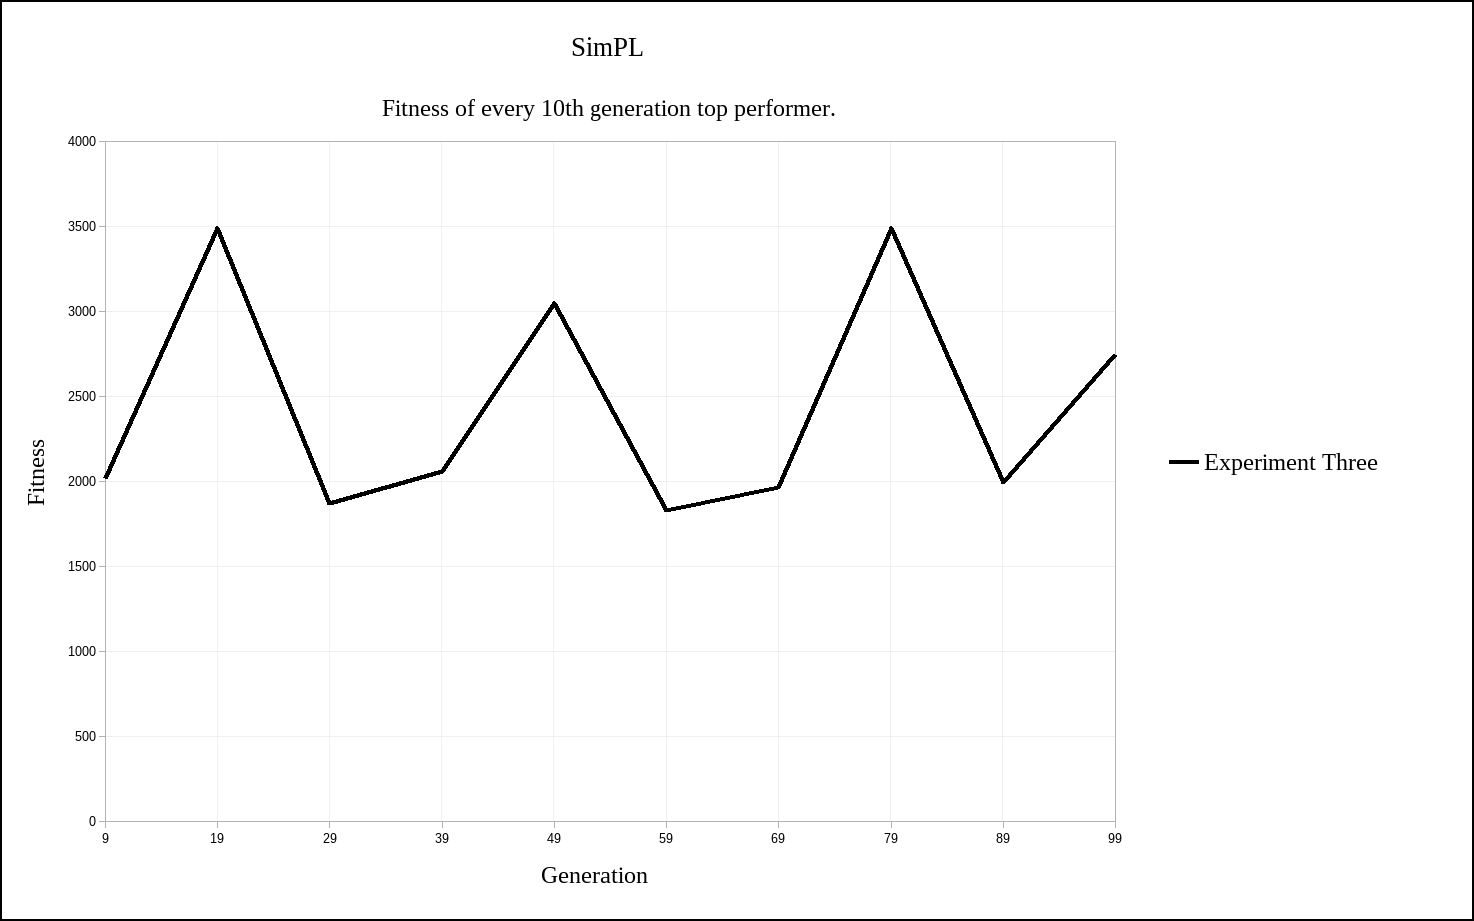
\includegraphics[width=5in]{../Figures/Chapter3/exp3_10_tops.png}
  \rule{35em}{0.5pt}
  \caption[Experiment Three Top Performers]{Here you see the fitness of every 10th generation top performer for experiment three.}
  \label{fig:exp3_10_tops}
\end{figure}

\begin{figure}[htbp]  
  \centering
  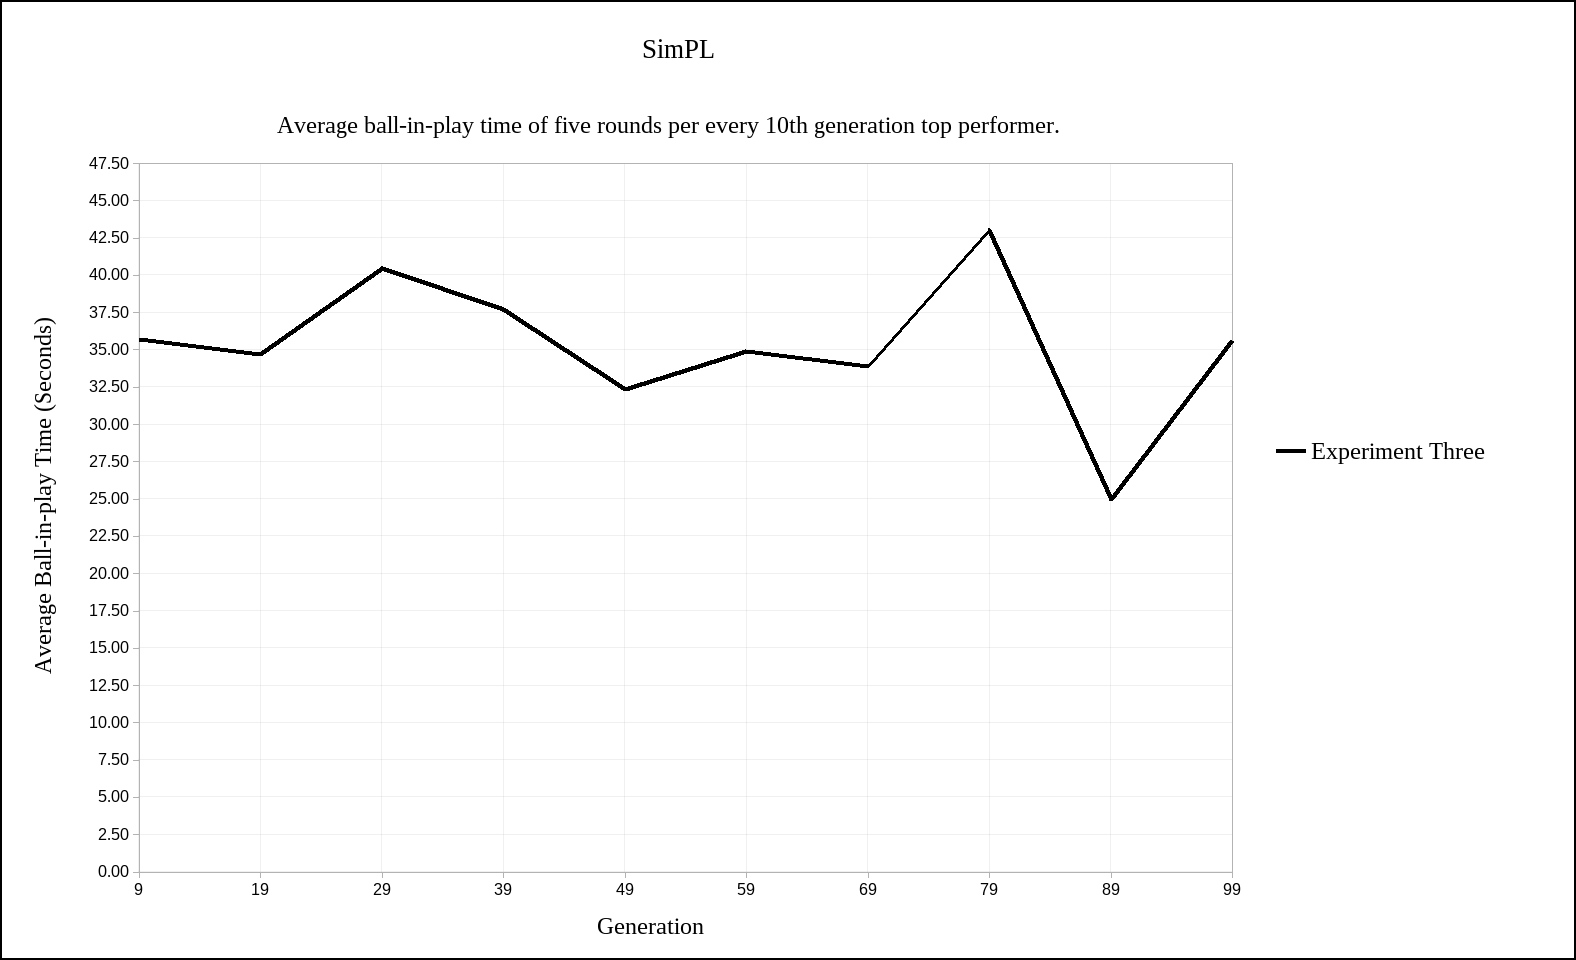
\includegraphics[width=5in]{../Figures/Chapter3/exp3_10_tops_times.png}
  \rule{35em}{0.5pt}
  \caption[Experiment Three Top Performers Tournament]{Here you see the average ball-in-play time (in seconds) of five rounds per every 10th generation top performer for experiment three.}
  \label{fig:exp3_10_tops_times}
\end{figure}

\subsection[Experiment Four]{Experiment four: static crossover and mutation probabilities with the crossover and mutation operators working in parallel.}

Experiment four (Figures \ref{fig:exp4_avg_fit}-\ref{fig:exp4_10_tops_times}) produces similar results, with initial improvement in average fitness for the first 10 generations, but oscillation thereafter. However, the mean of the average ball-in-play times was 37.28646 seconds, over the mean 35.33994 seconds shown for the player learned in Experiment three and the mean 34.18604 seconds in Experiment two.

\begin{figure}[htbp]  
  \centering
  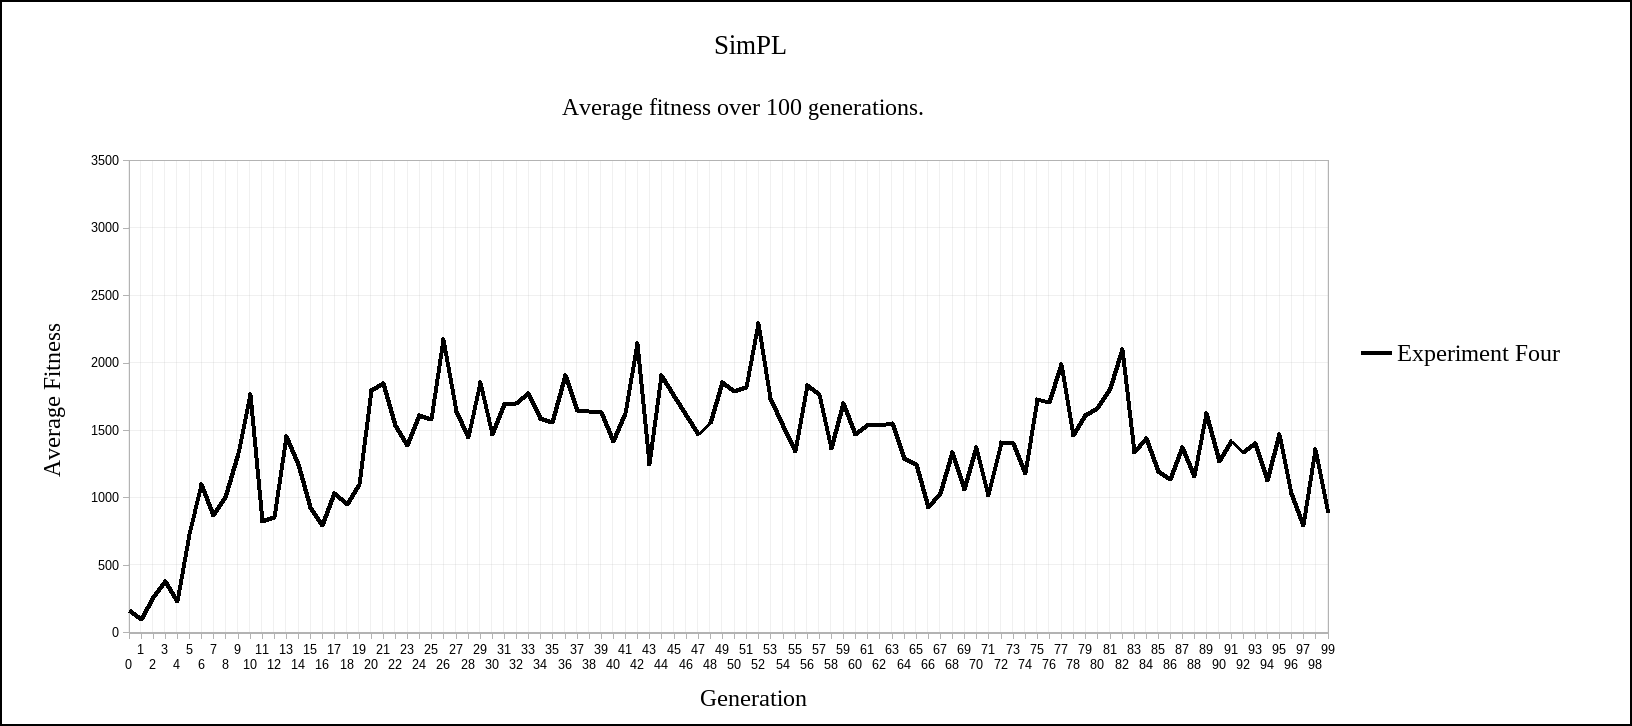
\includegraphics[width=5in]{../Figures/Chapter3/exp4_avg_fit.png}
  \rule{35em}{0.5pt}
  \caption[Experiment Four Average Fitness]{Here you see the average fitness over 100 generations for experiment four.}
  \label{fig:exp4_avg_fit}
\end{figure}

\begin{figure}[htbp]  
  \centering
  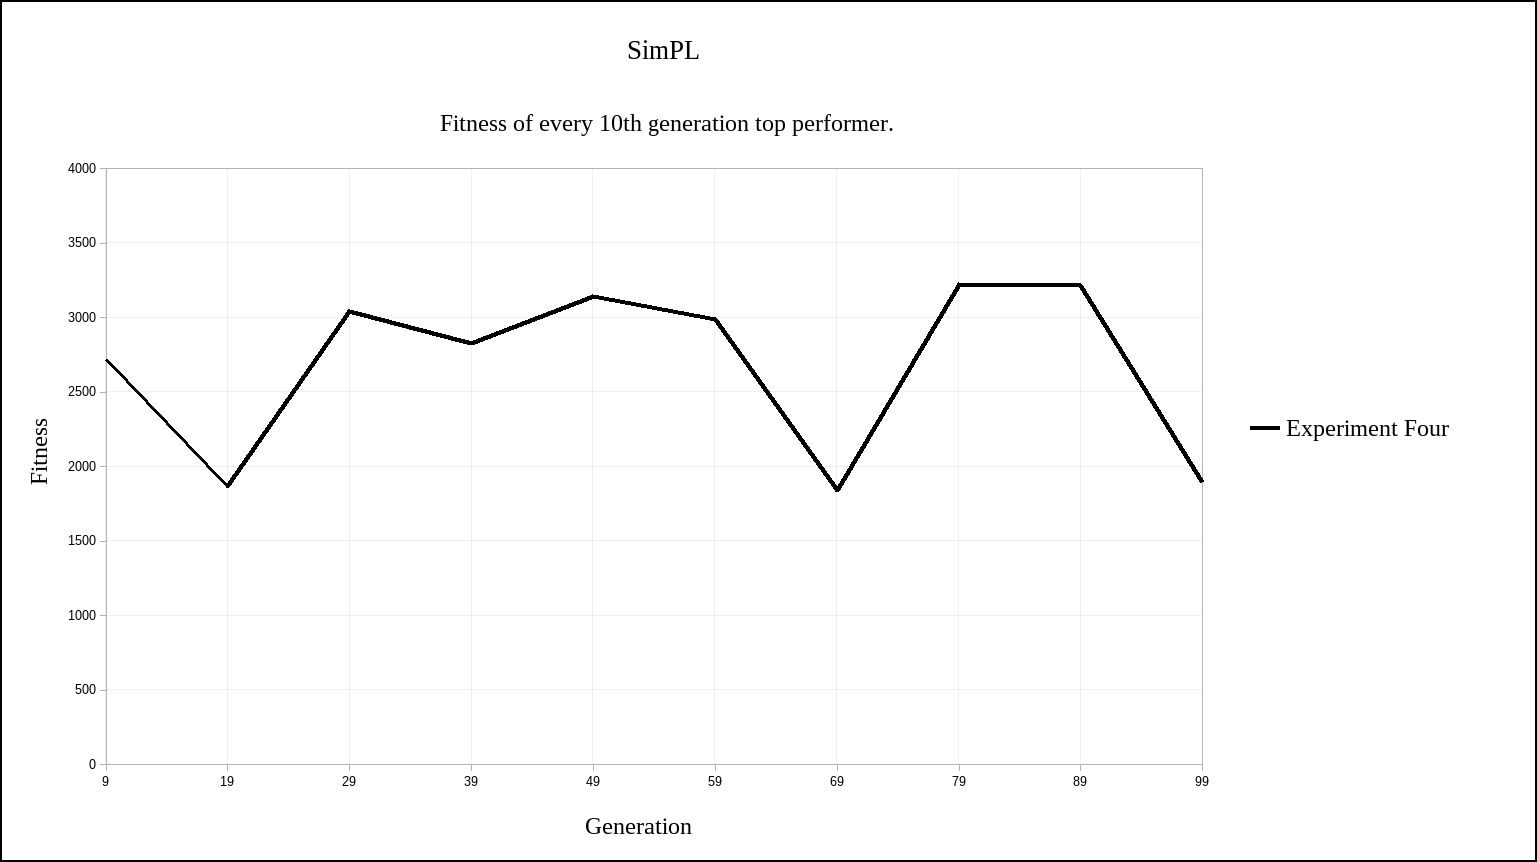
\includegraphics[width=5in]{../Figures/Chapter3/exp4_10_tops.png}
  \rule{35em}{0.5pt}
  \caption[Experiment Four Top Performers]{Here you see the fitness of every 10th generation top performer for experiment four.}
  \label{fig:exp4_10_tops}
\end{figure}

\begin{figure}[htbp]  
  \centering
  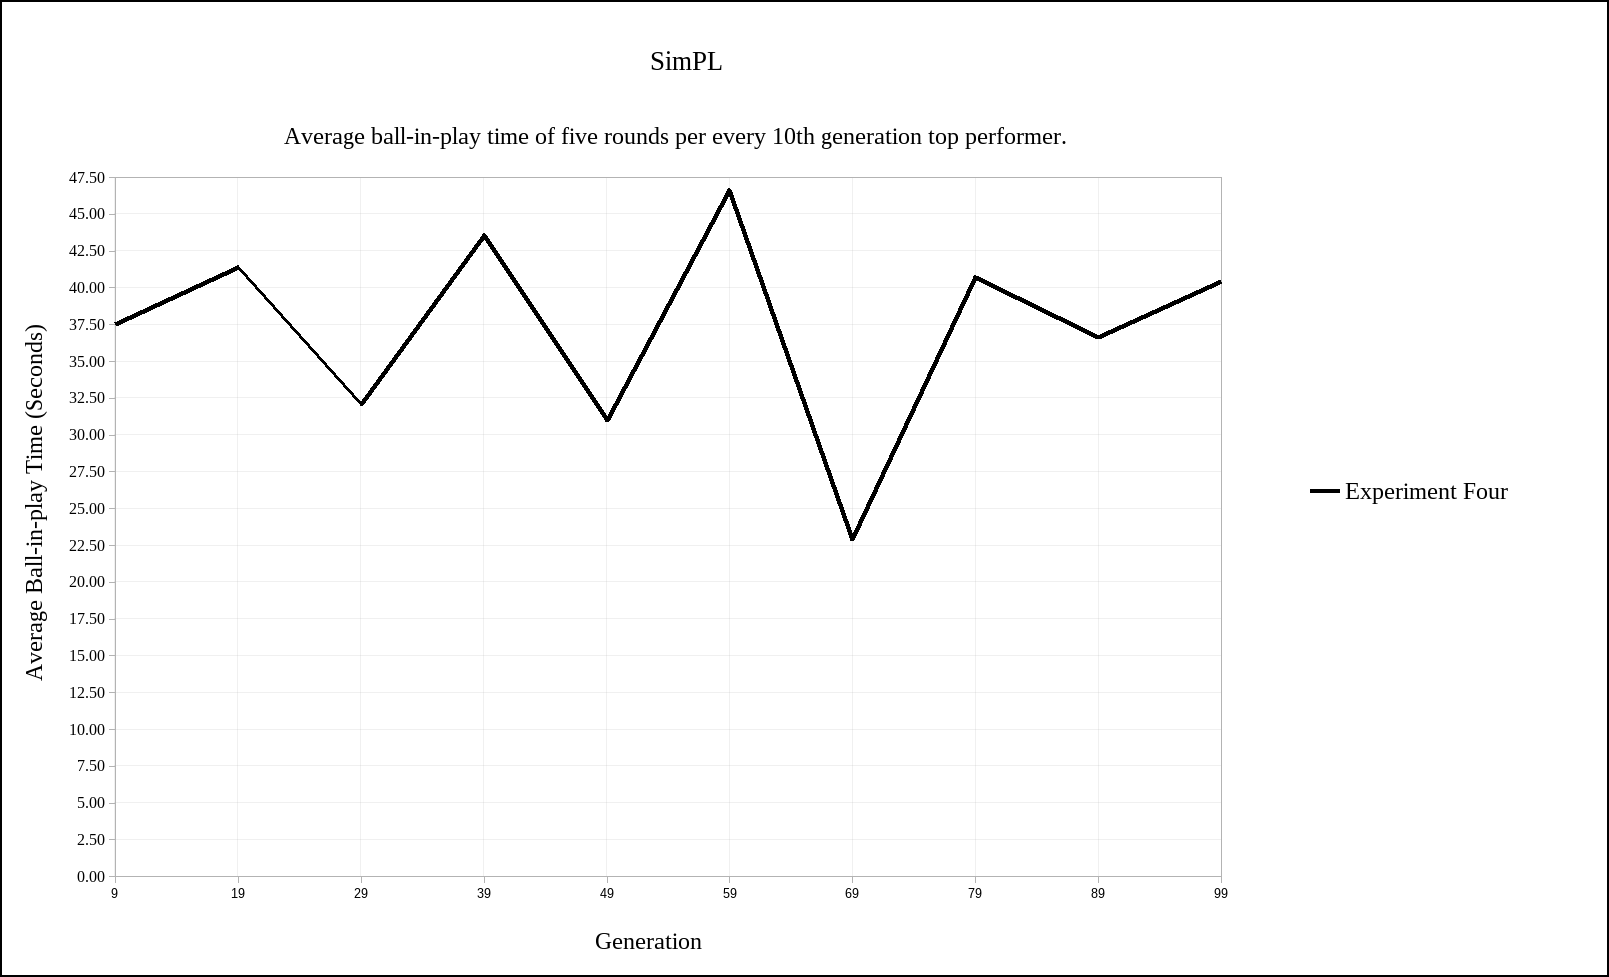
\includegraphics[width=5in]{../Figures/Chapter3/exp4_10_tops_times.png}
  \rule{35em}{0.5pt}
  \caption[Experiment Four Top Performers Tournament]{Here you see the average ball-in-play time (in seconds) of five rounds per every 10th generation top performer for experiment four.}
  \label{fig:exp4_10_tops_times}
\end{figure}

\subsection[Experiment Five]{Experiment five: static crossover and mutation probabilities with the crossover and mutation operators working in sequence.}

Experiment five (Figures \ref{fig:exp5_avg_fit}-\ref{fig:exp5_10_tops_times}) shows more gradual improvement in average fitness over the first 31 generations. Overall, the mean of the average ball-in-play times was 37.91126 seconds---higher than that of Experiment four.

\begin{figure}[htbp]  
  \centering
  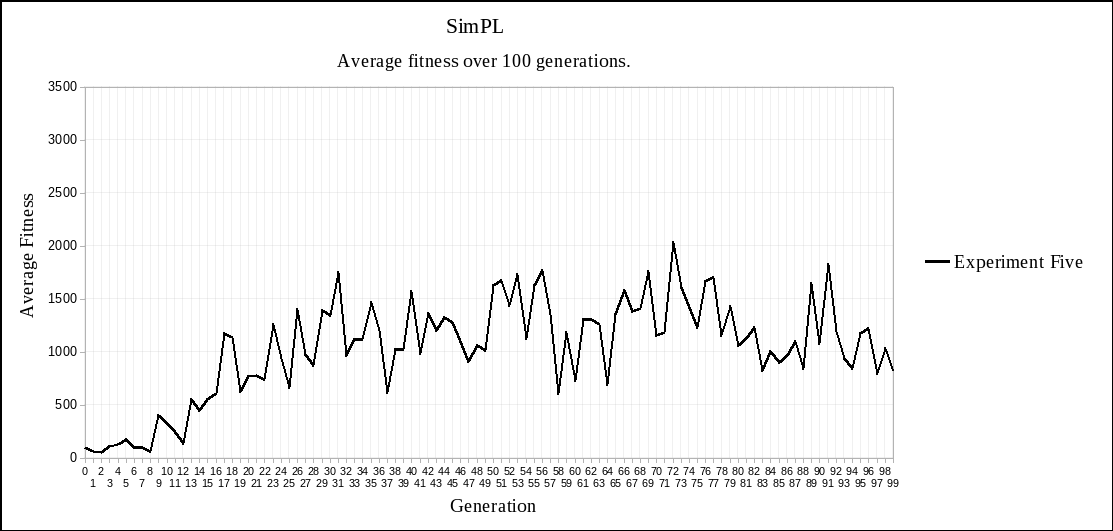
\includegraphics[width=5in]{../Figures/Chapter3/exp5_avg_fit.png}
  \rule{35em}{0.5pt}
  \caption[Experiment Five Average Fitness]{Here you see the average fitness over 100 generations for experiment five.}
  \label{fig:exp5_avg_fit}
\end{figure}

\begin{figure}[htbp]  
  \centering
  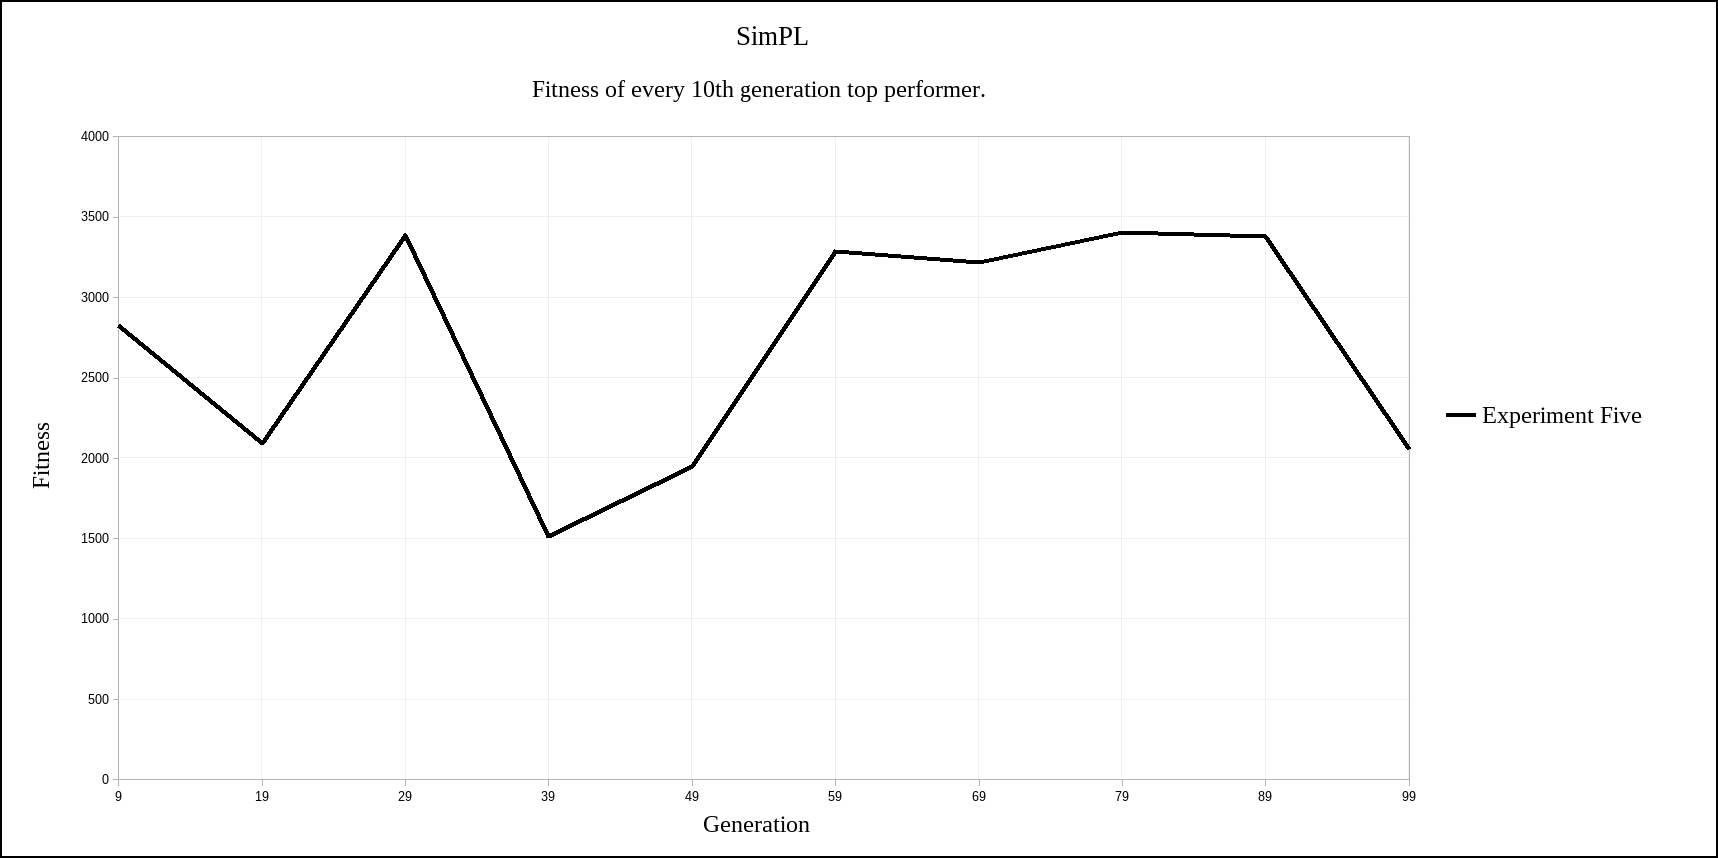
\includegraphics[width=5in]{../Figures/Chapter3/exp5_10_tops.png}
  \rule{35em}{0.5pt}
  \caption[Experiment Five Top Performers]{Here you see the fitness of every 10th generation top performer for experiment five.}
  \label{fig:exp5_10_tops}
\end{figure}

\begin{figure}[htbp]  
  \centering
  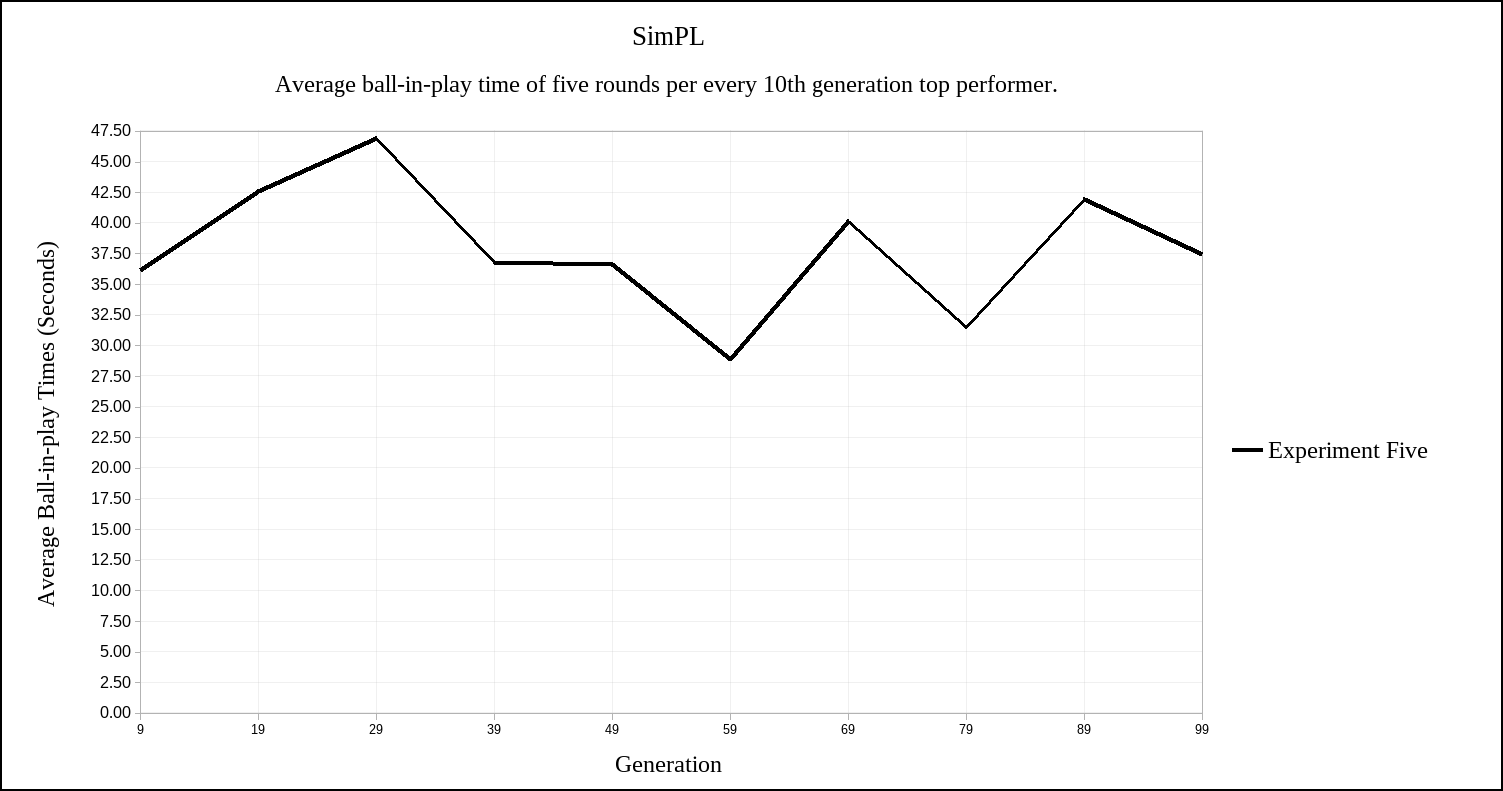
\includegraphics[width=5in]{../Figures/Chapter3/exp5_10_tops_times.png}
  \rule{35em}{0.5pt}
  \caption[Experiment Five Top Performers Tournament]{Here you see the average ball-in-play time (in seconds) of five rounds per every 10th generation top performer for experiment five.}
  \label{fig:exp5_10_tops_times}
\end{figure}

\subsection[Experiment Six]{Experiment six: fitness and ball-in-play upper bound.}

Experiment six (Figures \ref{fig:exp6_avg_fit}-\ref{fig:exp6_10_tops_times}) illustrates the \textit{perfect} results possible of a player who always behaves correctly. These metrics demonstrate optimal values, which can be considered targets for the evolution experiments. The mean of the average ball-in-play times was 40.01528 seconds, which means that Experiment five (above) comes closest to optimal performance.

\begin{figure}[htbp]  
  \centering
  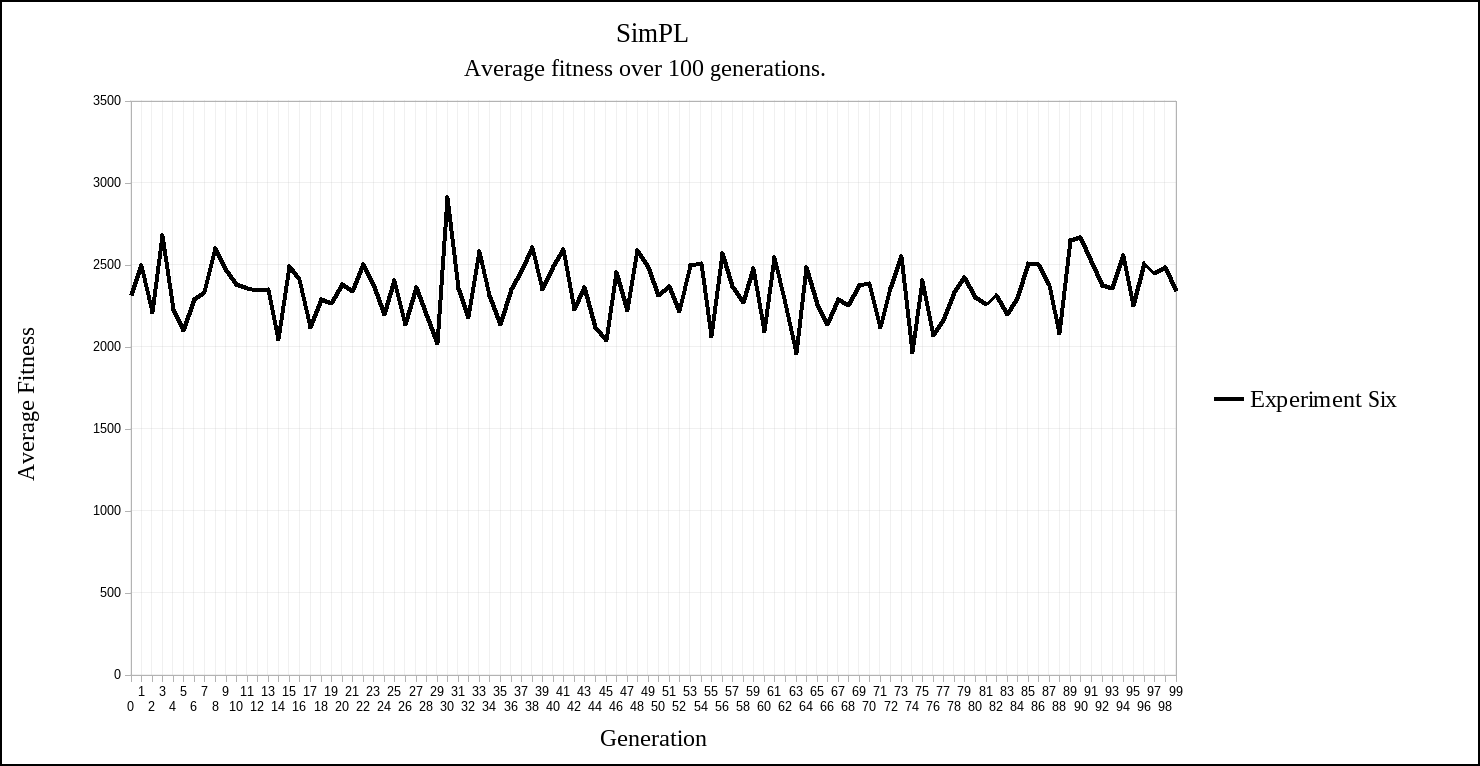
\includegraphics[width=5in]{../Figures/Chapter3/exp6_avg_fit.png}
  \caption[Experiment Six Average Fitness]{Here you see the average fitness over 100 generations for experiment six.}
  \label{fig:exp6_avg_fit}
\end{figure}

\begin{figure}[htbp]  
  \centering
  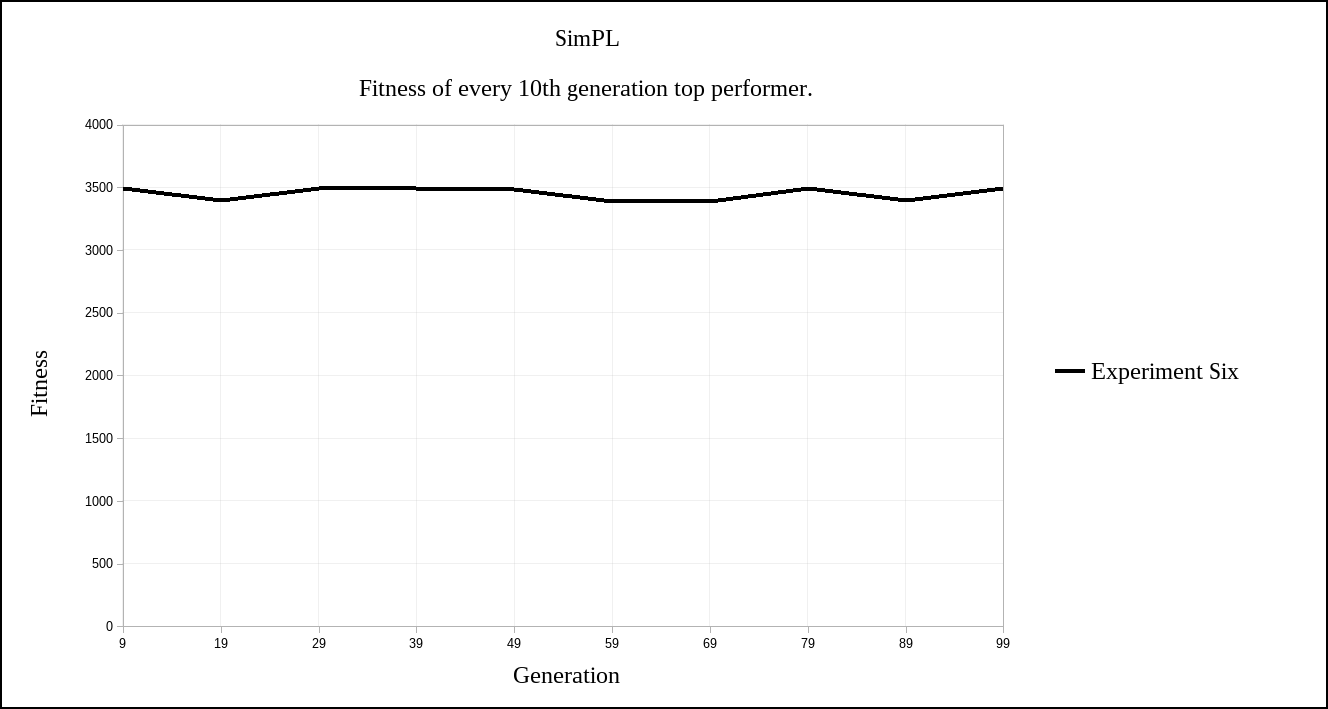
\includegraphics[width=5in]{../Figures/Chapter3/exp6_10_tops.png}
  \caption[Experiment Six Top Performers]{Here you see the fitness of every 10th generation top performer for experiment six.}
  \label{fig:exp6_10_tops}
\end{figure}

\begin{figure}[htbp]  
  \centering
  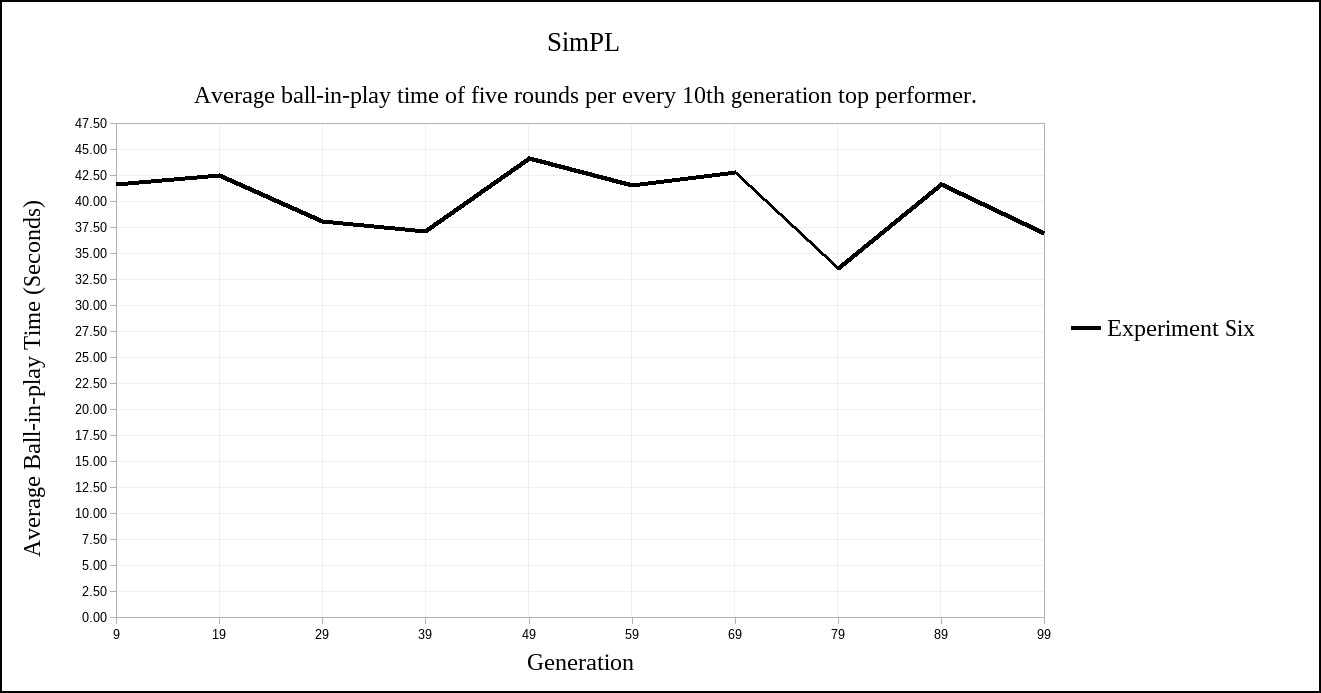
\includegraphics[width=5in]{../Figures/Chapter3/exp6_10_tops_times.png}
  \caption[Experiment Six Top Performers Tournament]{Here you see the average ball-in-play time (in seconds) of five rounds per every 10th generation top performer for experiment six.}
  \label{fig:exp6_10_tops_times}
\end{figure}

\subsection[Experiment Seven]{Experiment seven: random paddles.}

Experiment seven (Figures \ref{fig:exp7_avg_fit}-\ref{fig:exp7_10_tops_times}) illustrates the results of a player who behaves randomly. This provides an example of worst case metrics. The mean of the average average ball-in-play times was 5.2656 seconds, which is comparable to the first-generation games of the evolved players.

\begin{figure}[htbp]  
  \centering
  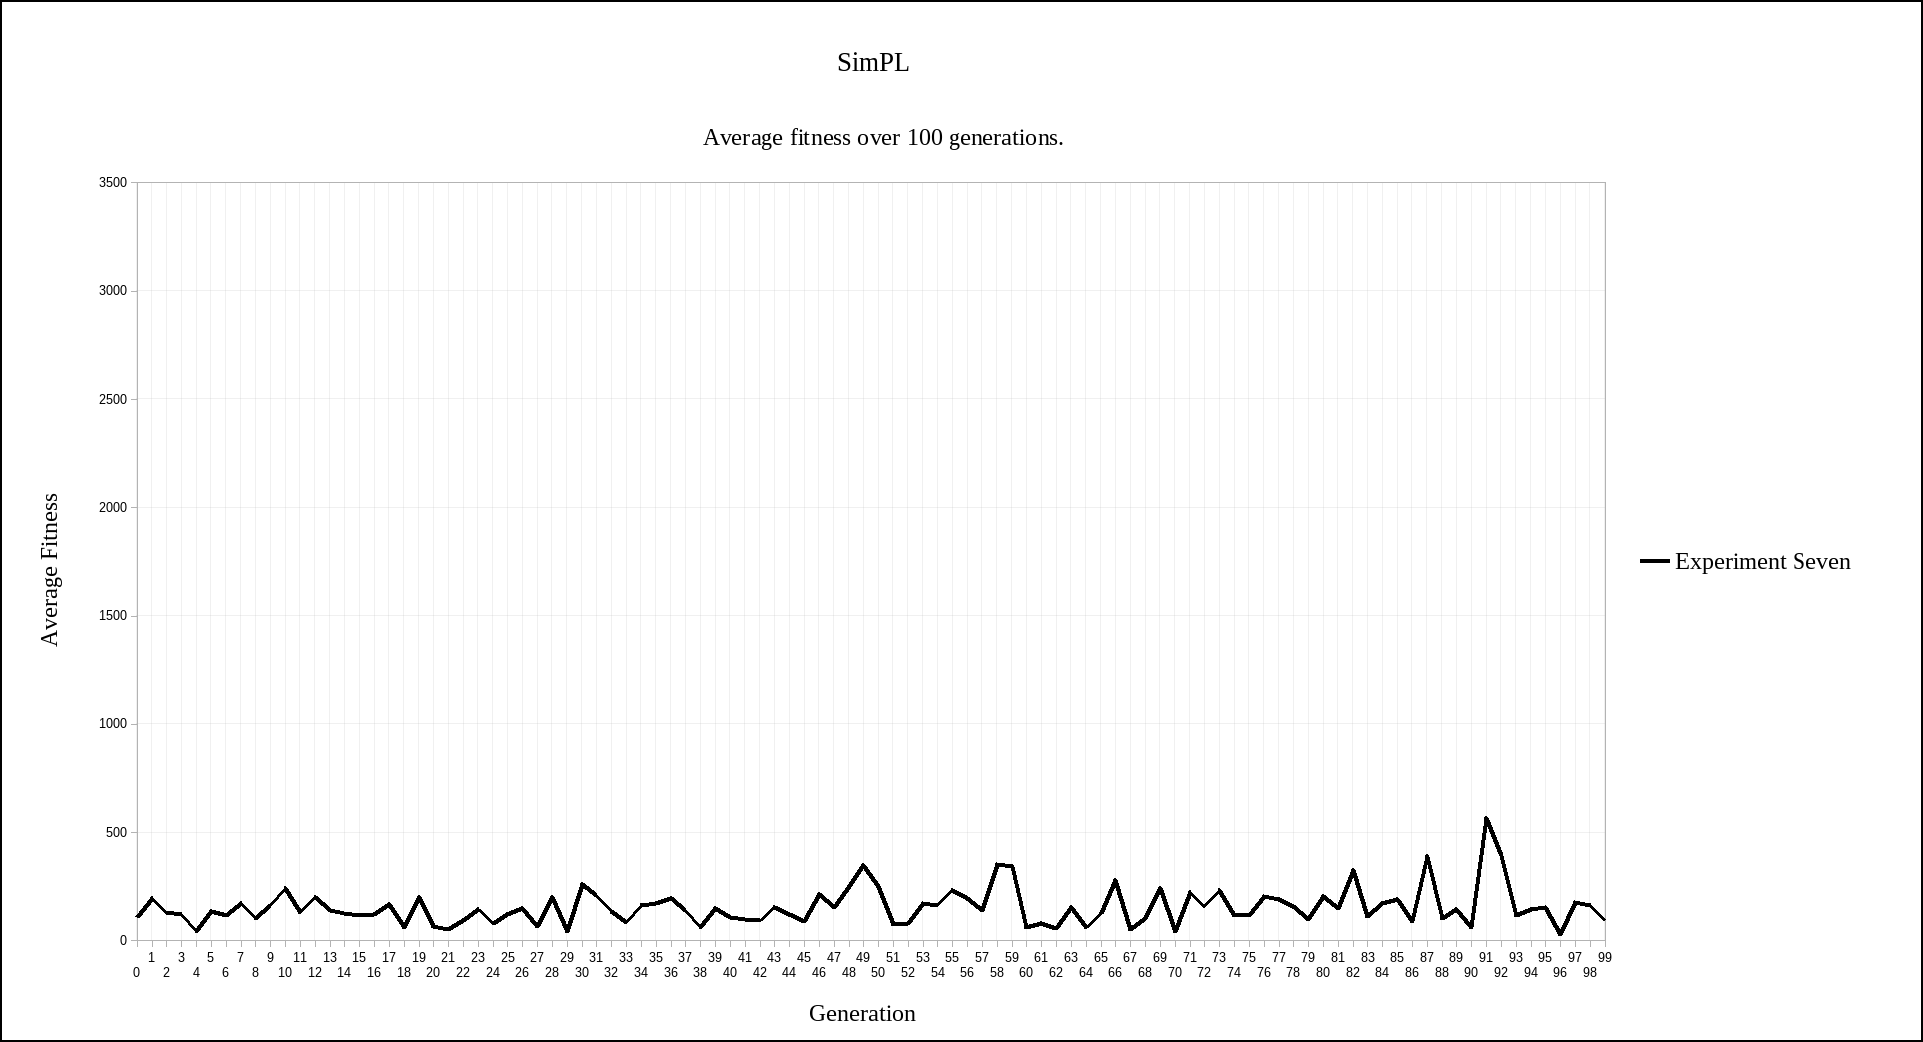
\includegraphics[width=5in]{../Figures/Chapter3/exp7_avg_fit.png}
  \caption[Experiment Seven Average Fitness]{Here you see the average fitness over 100 generations for experiment seven.}
  \label{fig:exp7_avg_fit}
\end{figure}

\begin{figure}[htbp]  
  \centering
  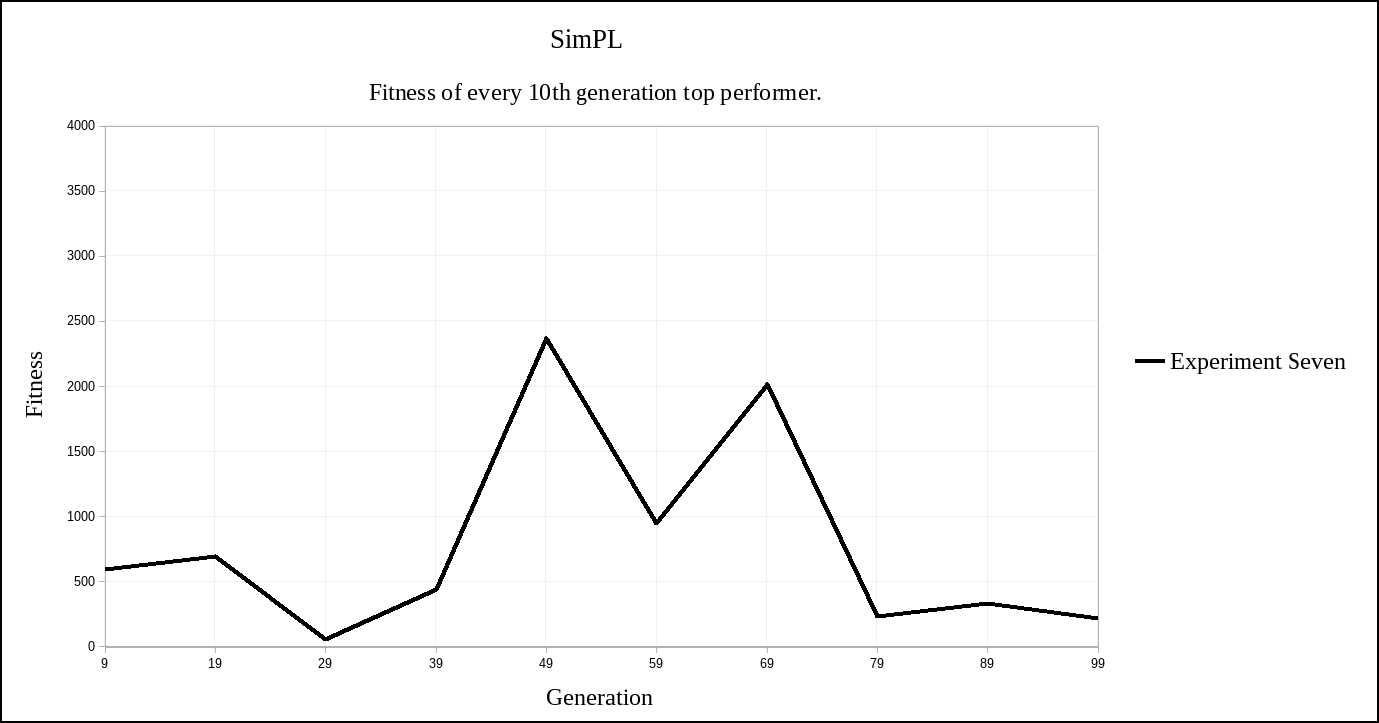
\includegraphics[width=5in]{../Figures/Chapter3/exp7_10_tops.png}
  \caption[Experiment Seven Top Performers]{Here you see the fitness of every 10th generation top performer for experiment seven.}
  \label{fig:exp7_10_tops}
\end{figure}

\begin{figure}[htbp]  
  \centering
  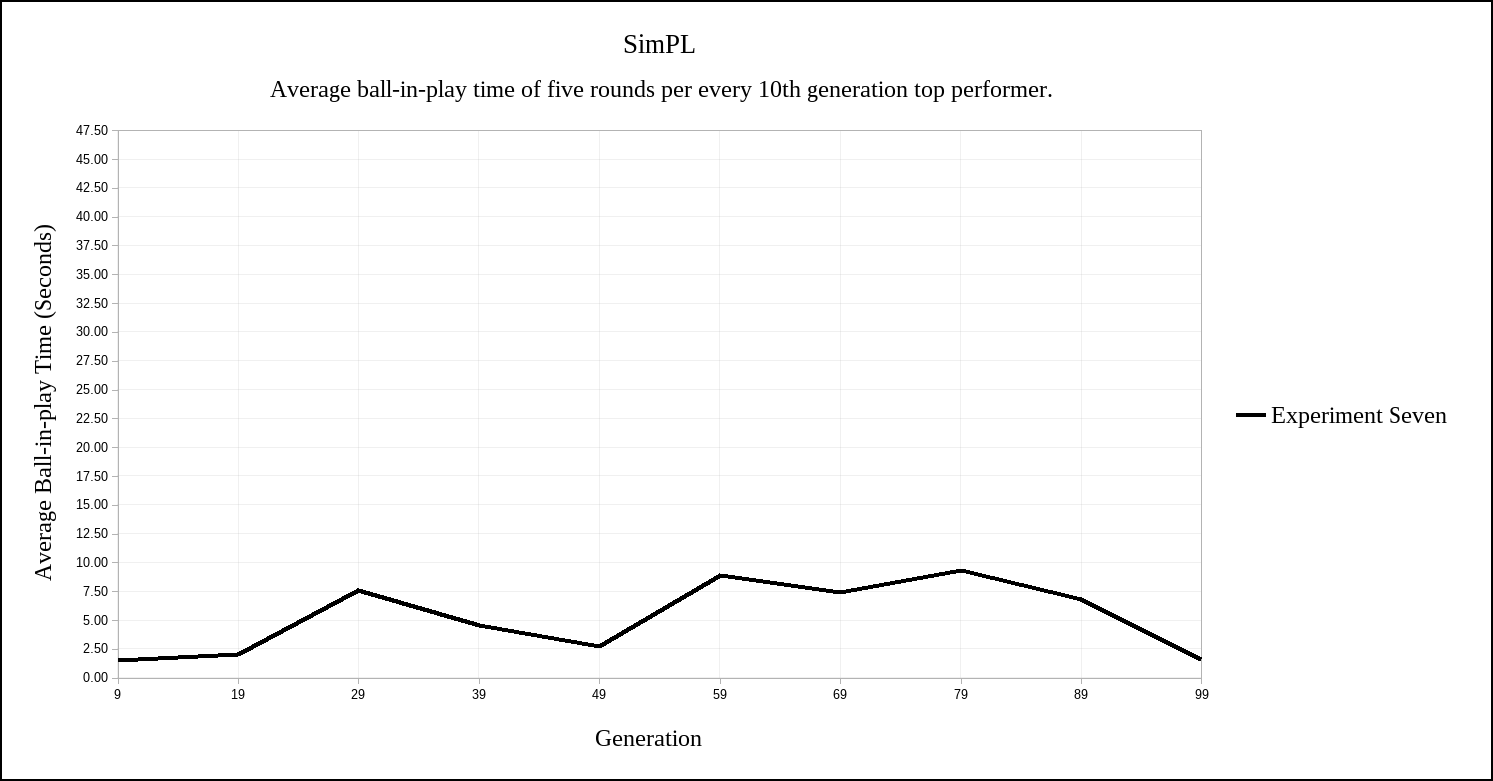
\includegraphics[width=5in]{../Figures/Chapter3/exp7_10_tops_times.png}
  \caption[Experiment Seven Top Performers Tournament]{Here you see the average ball-in-play time (in seconds) of five rounds per every 10th generation top performer for experiment seven.}
  \label{fig:exp7_10_tops_times}
\end{figure}

\subsection{Comparative Results}

This section illustrates comparative results by plotting all curves on the same axes (Figures \ref{fig:all_avg_fit} through \ref{fig:all_10_tops_times}).

\subsubsection{Average fitness over 100 generations.}

See Figure \ref{fig:all_avg_fit}.

\begin{figure}[htbp]  
  \centering
  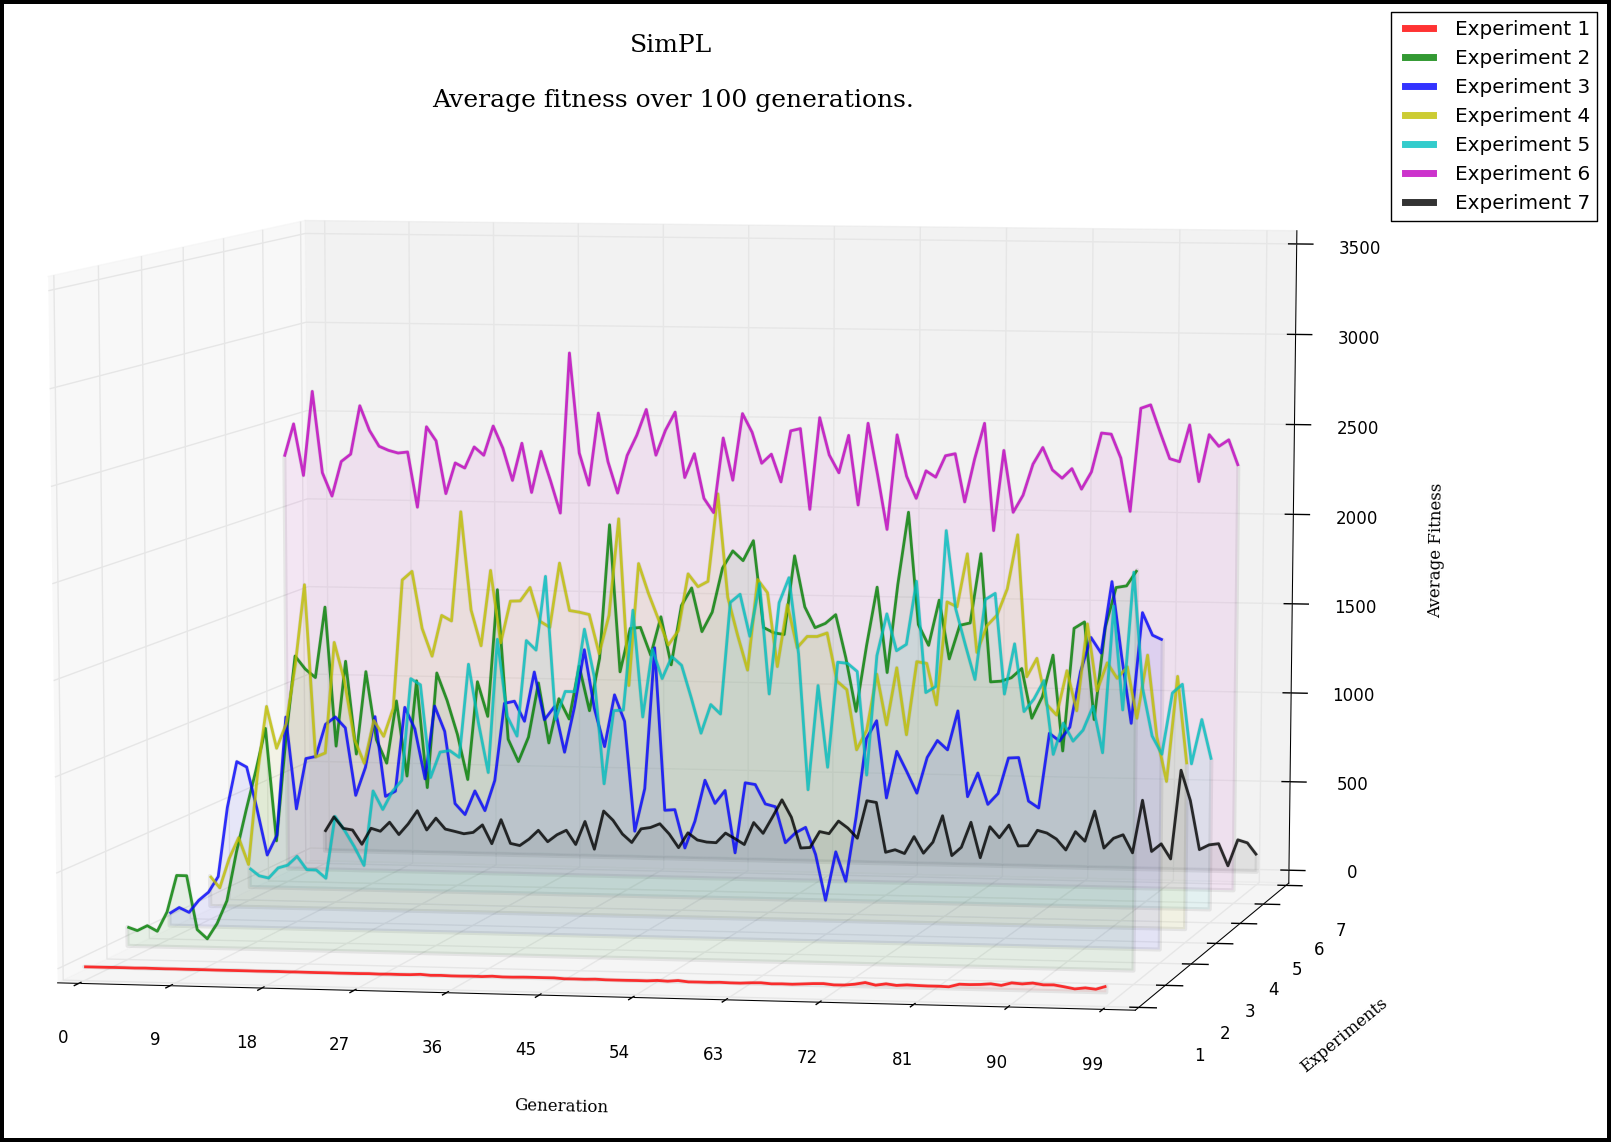
\includegraphics[width=5in]{../Figures/Chapter3/all_avg_fit.png}
  \rule{35em}{0.5pt}
  \caption[Average Fitness Composite]{Here you see the average fitness over 100 generations for experiments one through seven.}
  \label{fig:all_avg_fit}
\end{figure}

\subsubsection{Fitness of every 10th generation top performer.}

See Figure \ref{fig:all_10_tops}.

\begin{figure}[htbp]  
  \centering
  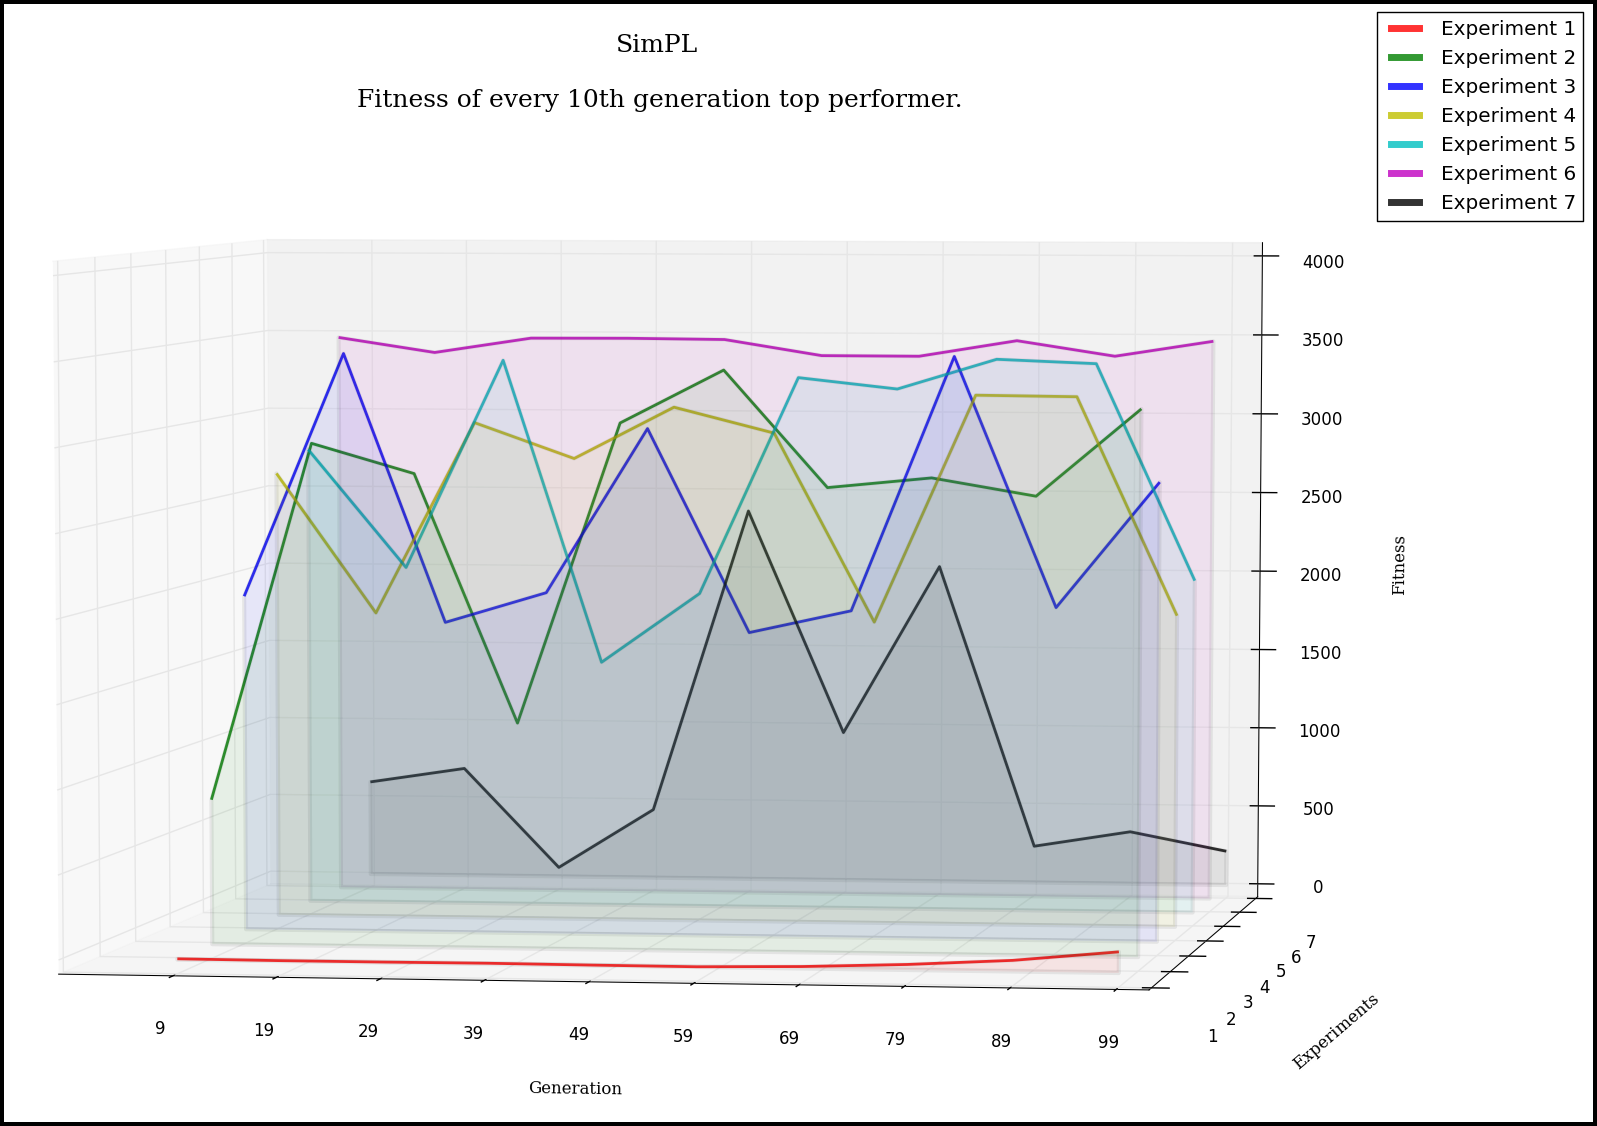
\includegraphics[width=5in]{../Figures/Chapter3/all_10_tops.png}
  \rule{35em}{0.5pt}
  \caption[Top Performers Composite]{Here you see the fitness of every 10th generation top performer for experiments one through seven.}
  \label{fig:all_10_tops}
\end{figure}

\subsubsection{Average ball-in-play time (in seconds) of five rounds per every 10th generation top performer.}

See Figure \ref{fig:all_10_tops_times}.

\begin{figure}[htbp]  
  \centering
  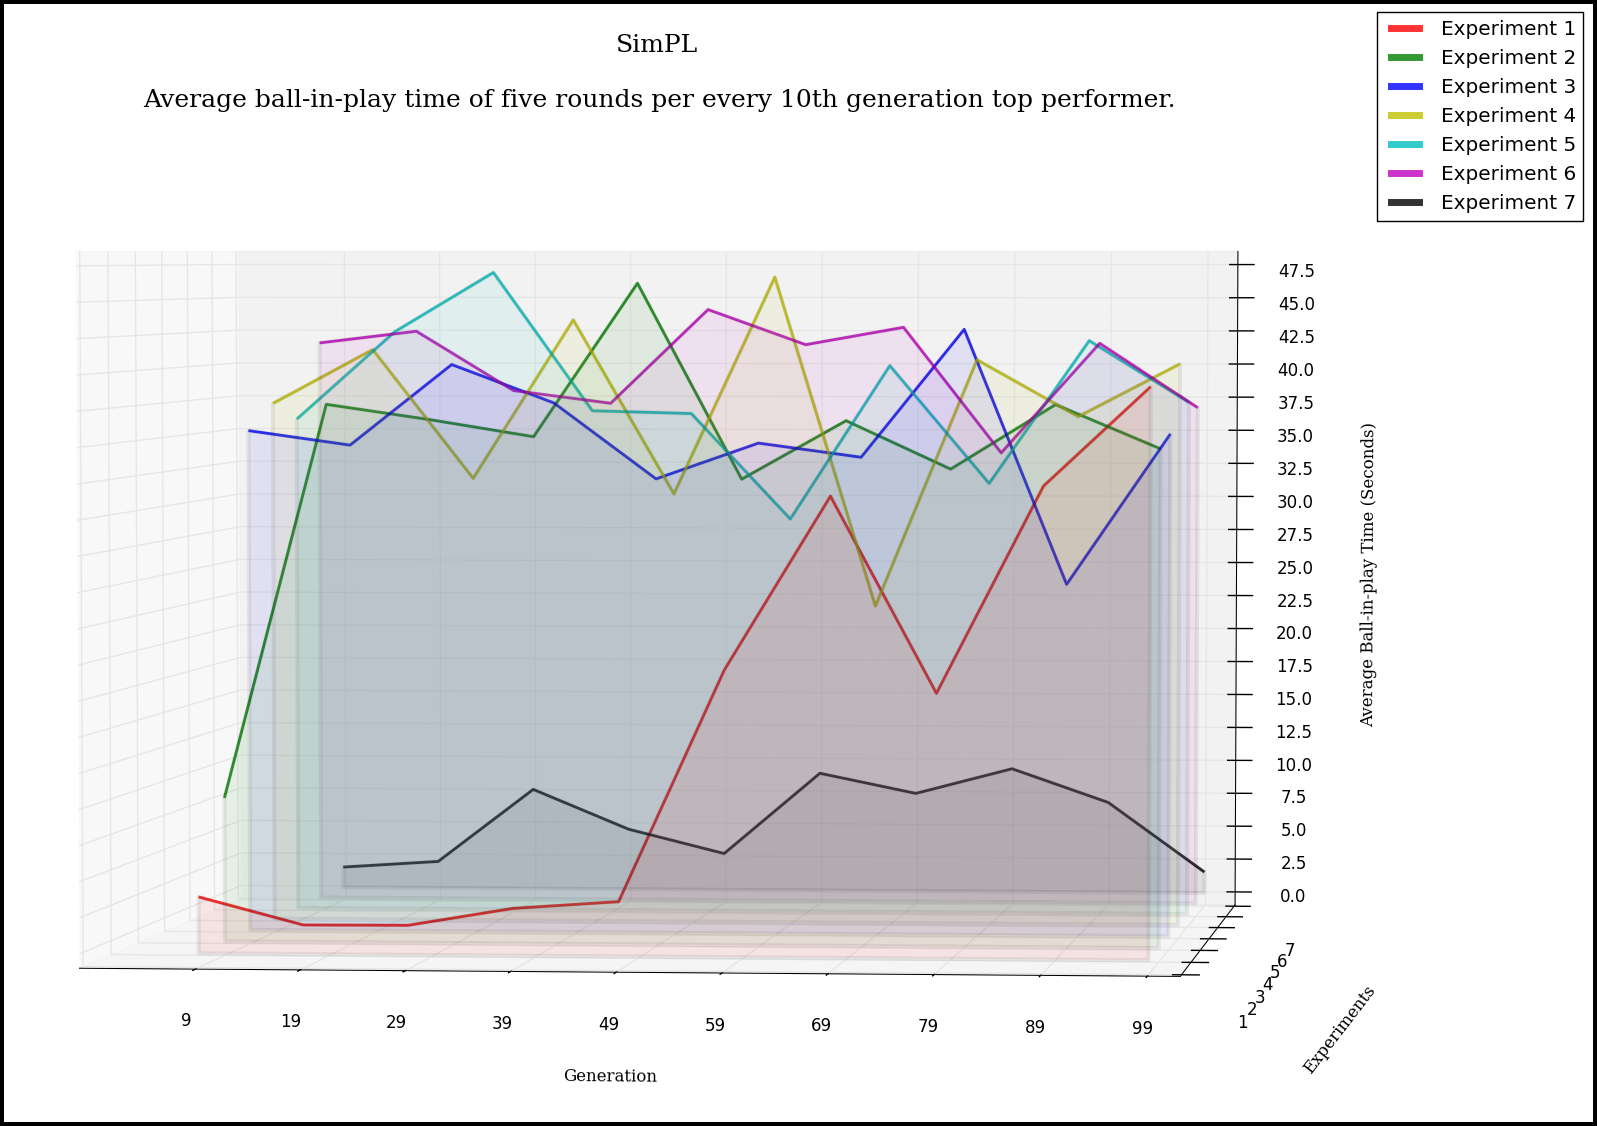
\includegraphics[width=5in]{../Figures/Chapter3/all_10_tops_times.png}
  \rule{35em}{0.5pt}
  \caption[Top Performers Tournament Composite]{Here you see the average ball-in-play time (in seconds) of five rounds per every 10th generation top performer for experiments one through seven.}
  \label{fig:all_10_tops_times}
\end{figure}

%\subsection{Experiment three, four, and five.}

%\begin{figure}[H]  
%  \centering
%  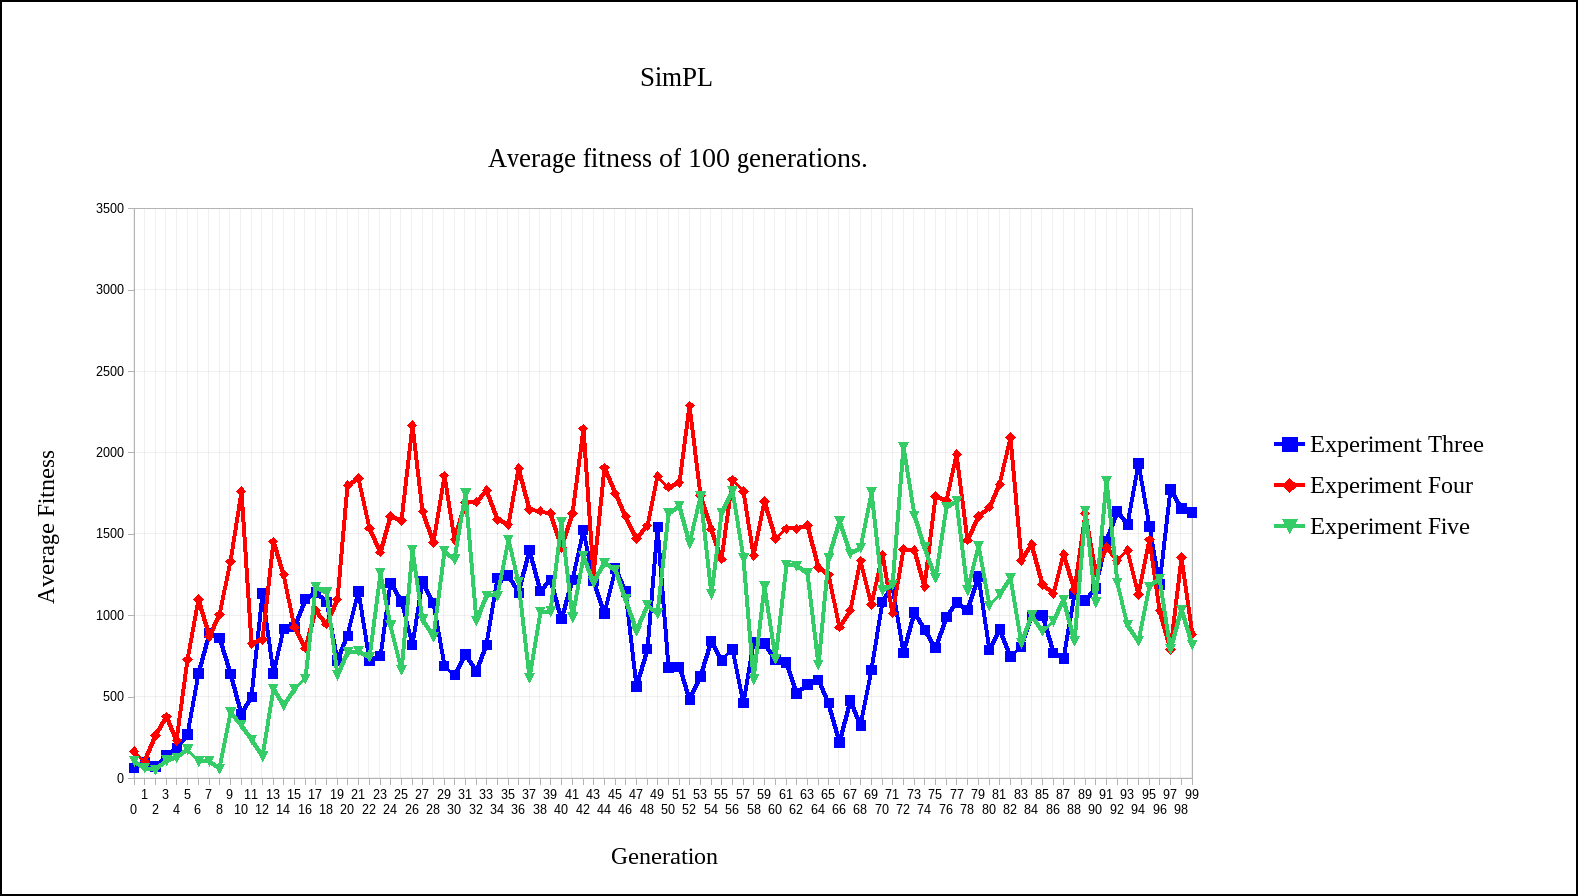
\includegraphics[width=1\textwidth]{exp345_avg_fit.png}
%  \caption{Here you see the average fitness over 100 generations for experiment three, four, and five.}
%  \label{fig:exp345_avg_fit}
%\end{figure}

%\begin{figure}[H]  
%  \centering
%  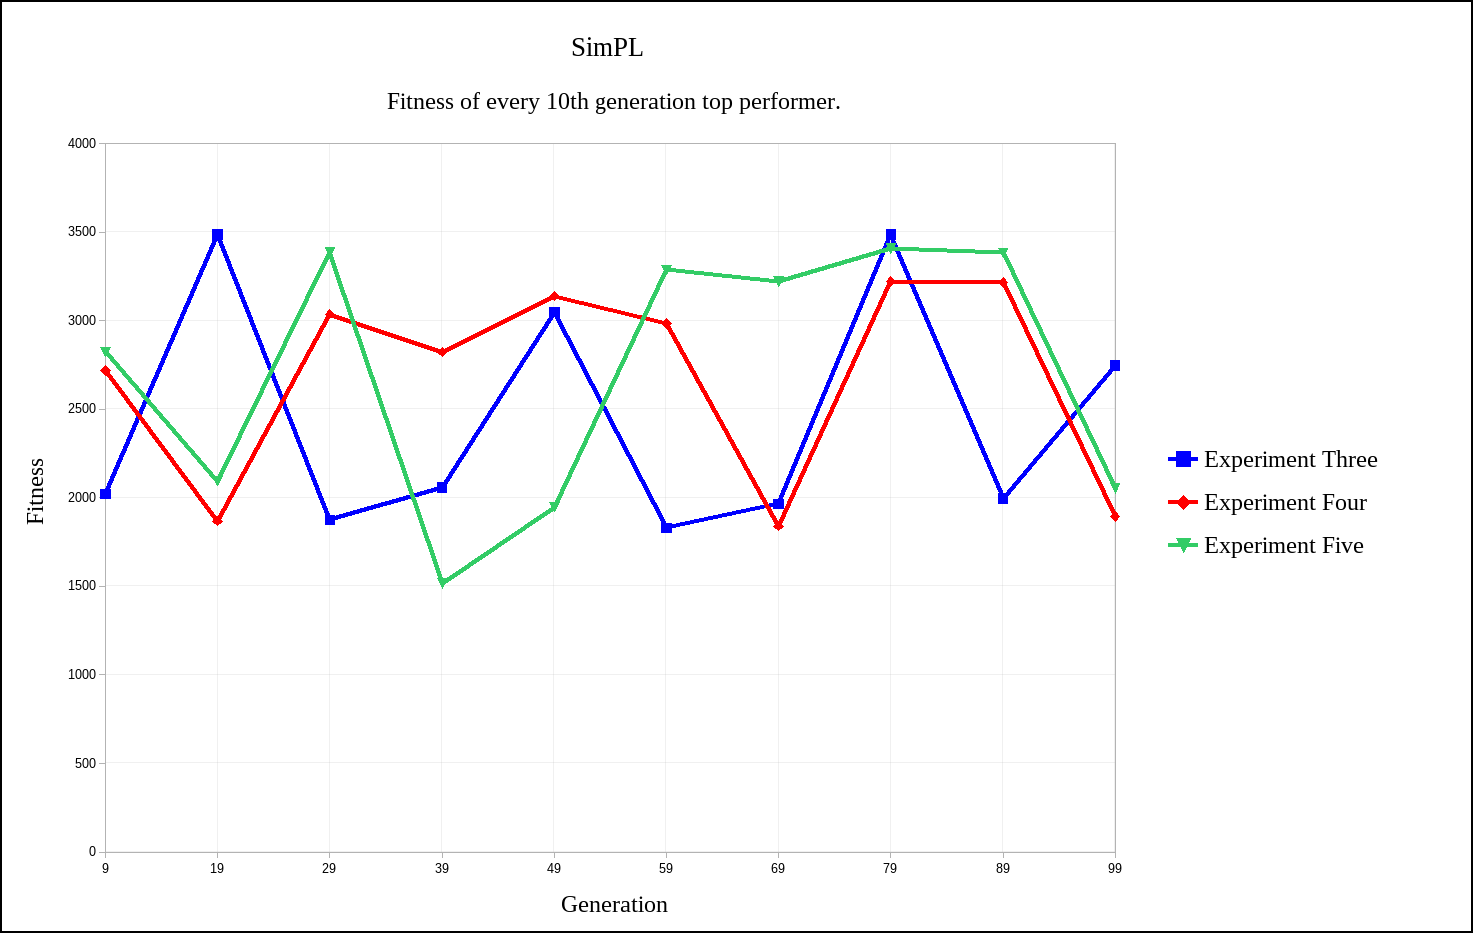
\includegraphics[width=1\textwidth]{exp345_10_tops.png}
%  \caption{Here you see the fitness of the every 10th generation top performer for experiment three, four, and five.}
%  \label{fig:exp345_10_tops}
%\end{figure}

%\begin{figure}[H]  
%  \centering
%  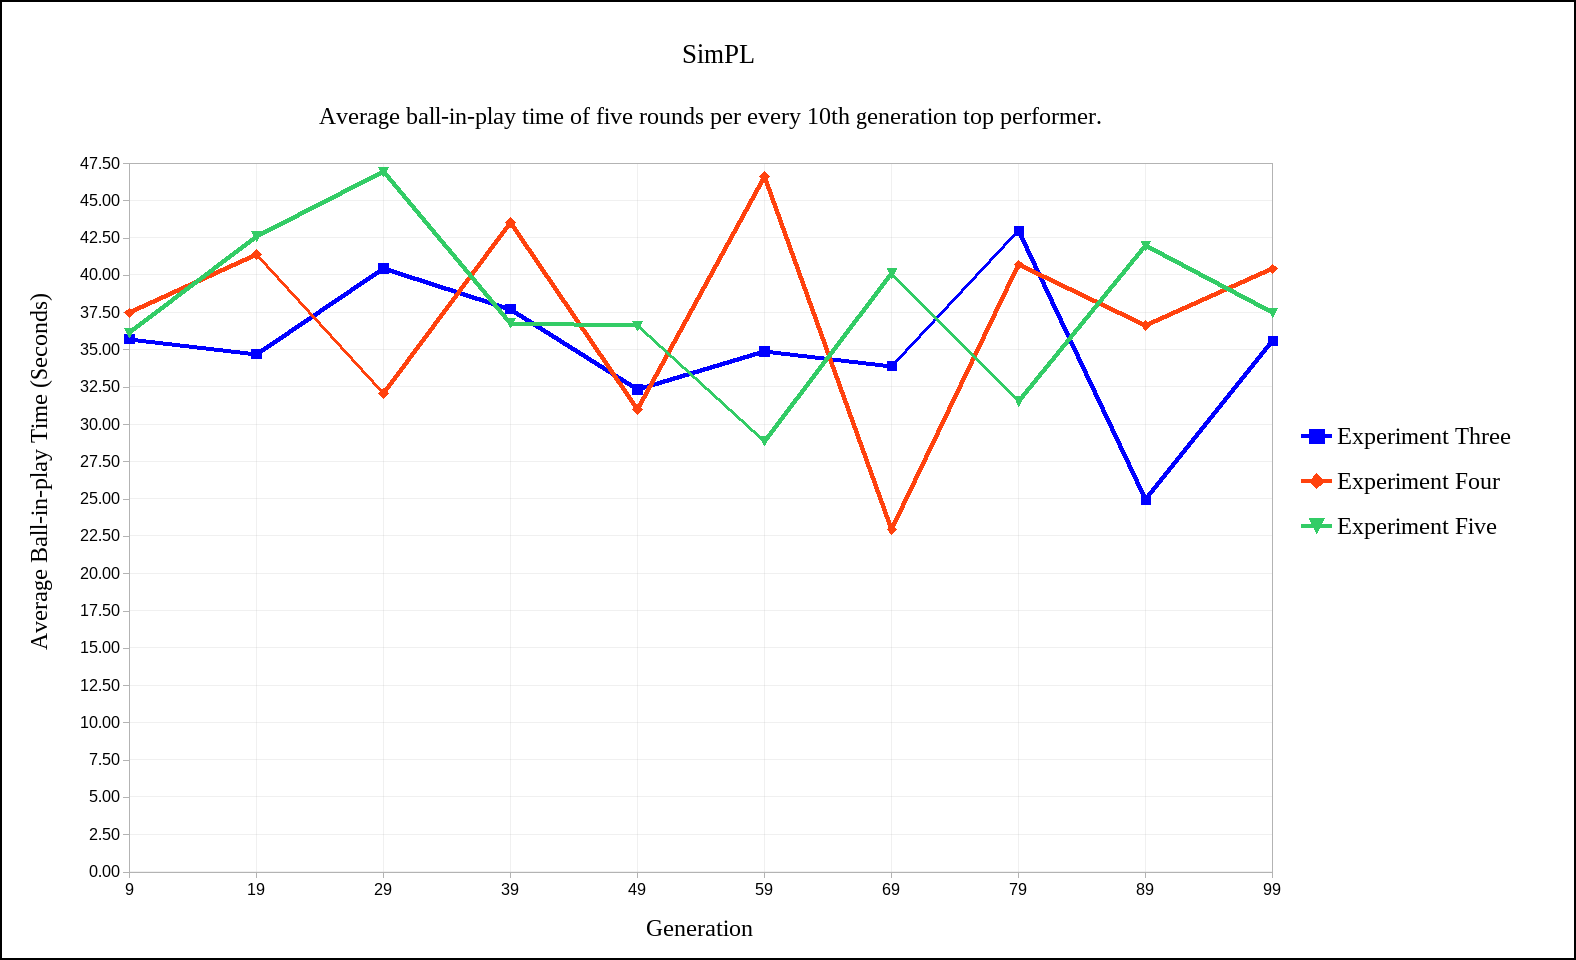
\includegraphics[width=1\textwidth]{exp345_10_tops_times.png}
%  \caption{Here you see the average ball-in-play time (in seconds) of five rounds per every 10th generation top performer for experiment three, four, and five.}
%  \label{fig:exp345_10_tops_times}
%\end{figure}

%\subsection{Experiment four, five, and six.}

%\begin{figure}[H]  
%  \centering
%  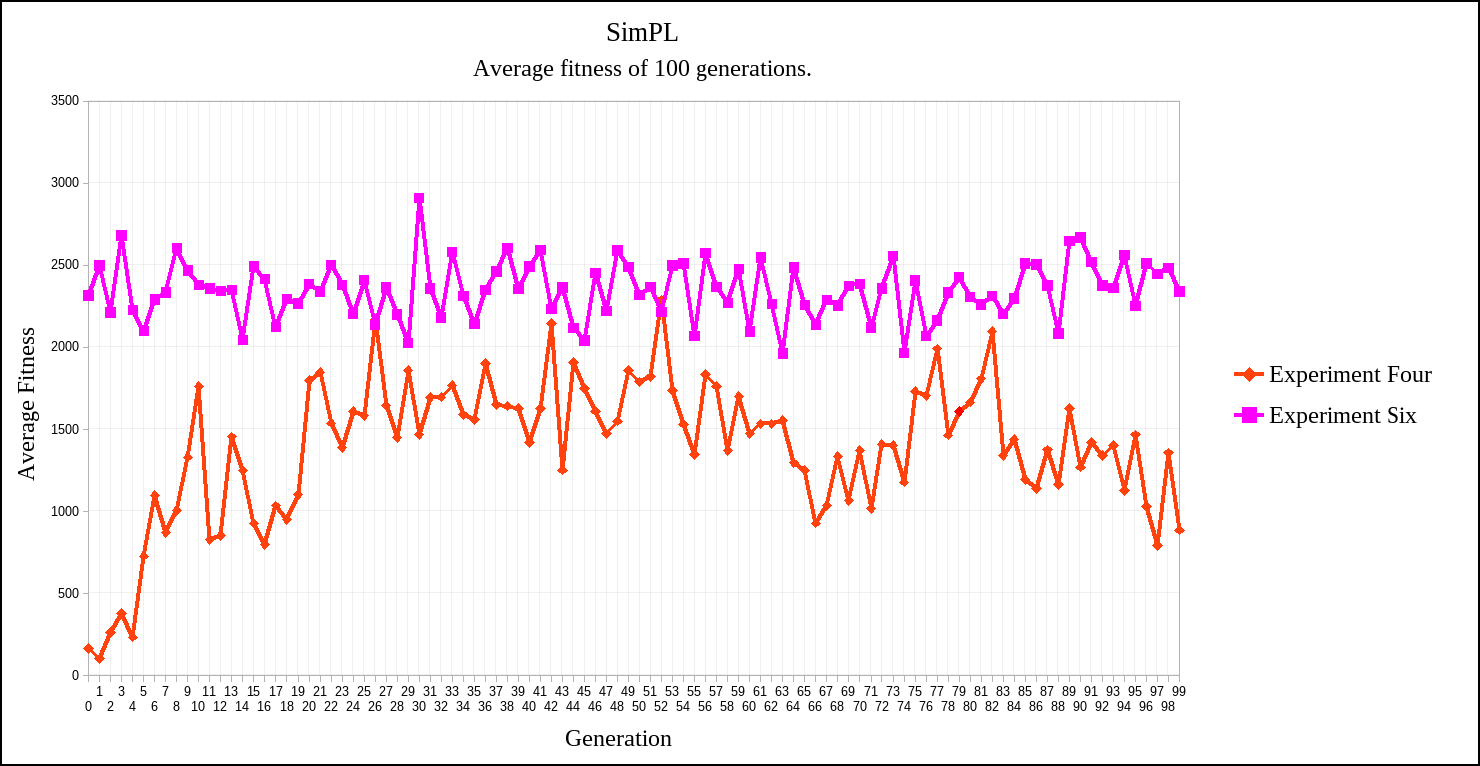
\includegraphics[width=1\textwidth]{exp46_avg_fit.png}
%  \caption{Here you see the average fitness over 100 generations for experiment four and six.}
%  \label{fig:exp46_avg_fit}
%\end{figure}

%\begin{figure}[H]  
%  \centering
%  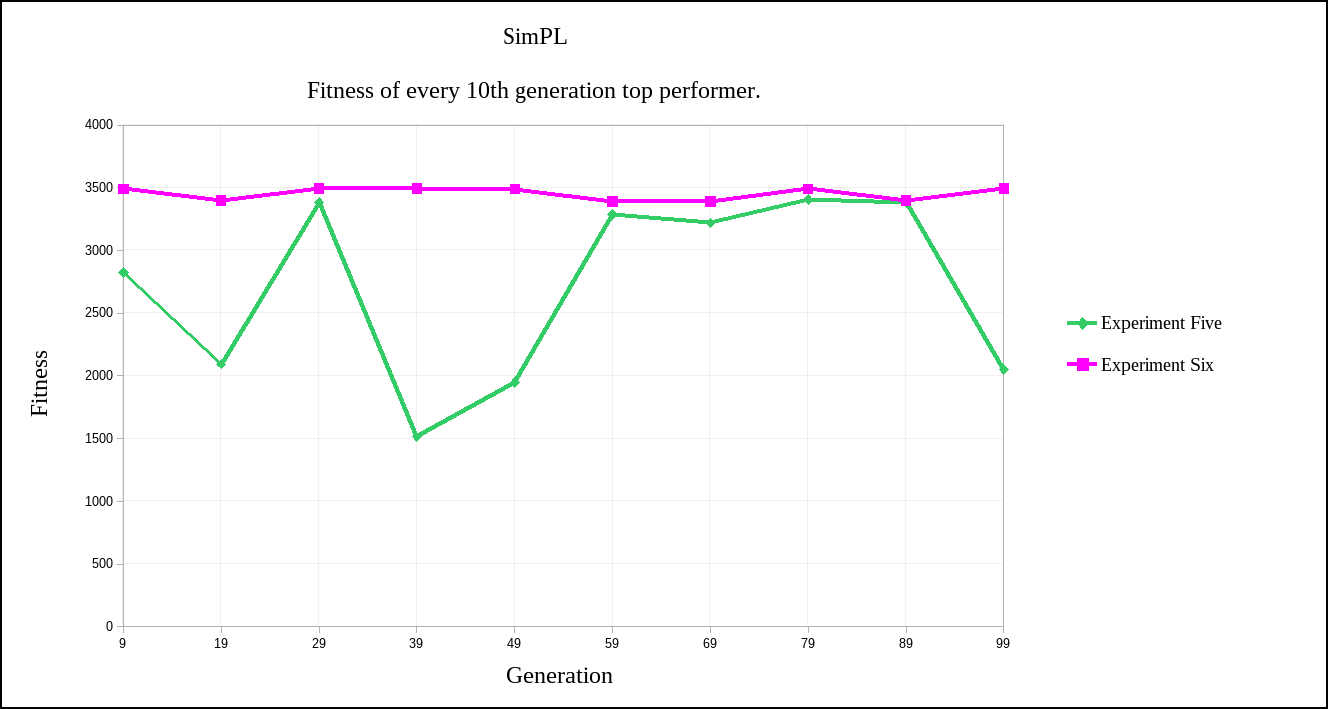
\includegraphics[width=1\textwidth]{exp56_10_tops.png}
%  \caption{Here you see the fitness of the every 10th generation top performer for experiment five and six.}
%  \label{fig:exp56_10_tops}
%\end{figure}

%\begin{figure}[H]  
%  \centering
%  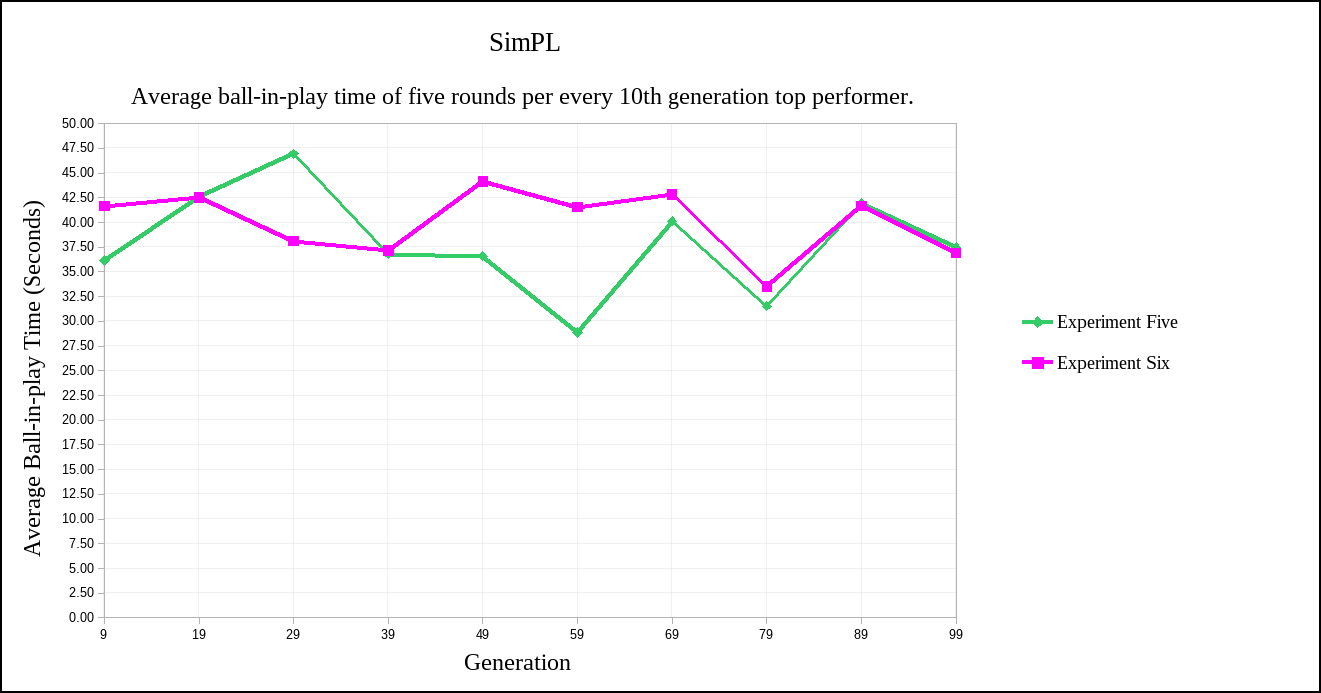
\includegraphics[width=1\textwidth]{exp56_10_tops_times.png}
%  \caption{Here you see the average ball-in-play time (in seconds) of five rounds per every 10th generation top performer for experiment five and six.}
%  \label{fig:exp56_10_tops_times}
%\end{figure}

%\subsection{Experiment one, two, three, four, five, six, and seven.}

\section{Conclusion}

\todo{Change the wording to reflect that it \textit{was} helpful to do SimPL since BBAutoTune was successful.}

The genetic algorithm developed for SimPL should prove to be a robust basis for the genetic algorithm needed to solve a harder problem of tuning a 3D physics engine (project BBAutoTune). The principles and techniques of evolutionary algorithms learned during the SimPL project will certainly carry over to the more difficult project, BBAutoTune. And while the problem domain of SimPL and BBAutoTune are only somewhat similar, the problems faced and worked out during the development of SimPL should alleviate problems faced while developing BBAutoTune. As the results show, the genetic algorithm for SimPL performed well, producing neural network weight solutions that had the paddle keeping the ball in the arena for almost a minute. Had it not been for the round termination criteria of the ball's velocity magnitude dropping below $100$, most of the paddles (with high fitnesses) would have kept the ball in the arena indefinitely. Thus, the goal to learn about and to cultivate a genetic algorithm capable of tuning parameters with respect to a fitness landscape was certainly accomplished. 
  \chapter{BBAutoTune}

\label{Chapter4}

\section{Overview}

The purpose of BBAutoTune is to find the correct combination of physics parameters such that the motion of the simulated robot is indistinguishable from the real world counterpart. Components of BBAutoTune include a genetic algorithm, database manager, GUI panel, and an external progress monitor which tracks various metrics of the running genetic algorithm.  

\section{Implementation}

Most of the components to BBAutoTune run inside of Blender itself with the exception of the external GA monitor. Blender's API uses the Python programming language and thus BBAutoTune was written entirely in Python. 

\subsection{Surveyor SRV-1 Blackfin 3D Model}

The robot used during experimentation was a 3D model of the Surveyor SRV-1 Blackfin. This model is dimensionally and aesthetically based on the real robot. The extents of the model are $17.64cm\times14.54cm\times14.33cm$ including the braille hat that rests above the body of the robot. The base and the wheels are the only physics based objects on the model with the wheels being connected to the base via a rigid body hinge joint. See Figure \ref{fig:srv1_3d_model}.

\subsection{GUI}

Blender's graphical user interface can be extended via its Python API. BBAutoTune adds a custom panel to Blender that allows the user to specify certain parameters pertaining to the GA and the overall tuning loop. Once the user specifies their preferred parameters, they press start to begin the tuning process. After pressing start, BBAutoTune will continue to run until the GA has reached the max generations specified. See Figure \ref{fig:bbautotune_gui}. 

\begin{figure}[htbp]
\centering
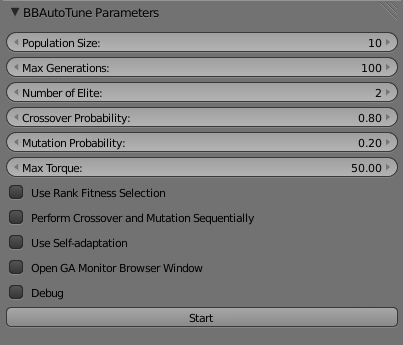
\includegraphics[scale=0.6]{../Figures/Chapter4/bbautotune_gui.png}
\rule{35em}{0.5pt}
\caption[BBAutoTune GUI Panel]{Here you see the BBAutoTune GUI panel added to Blender.}
\label{fig:bbautotune_gui}
\end{figure}

\subsection{Physics Engine API}

Blender exposes the Bullet\footnote{Bullet is the real time physics engine used by Blender. Released under the zlib license, Bullet provides real time continuous collision detection and rigid body dynamics \cite{website:continuousphysics}.} physics engine API via its own Python API. Most if not all of the parameters to Bullet can be modified via the physics engine API during or before running the Blender game engine. There are 41 different physics engine parameters that can be set via the API.

\subsubsection{Parameter Set and Ranges}

See Table \ref{tab:physics_params_ranges}.

\begin{table}[htbp]
\centering
\footnotesize
\bgroup
\def\arraystretch{1.1}
\begin{tabular}{ | >{\centering\arraybackslash}m{4cm} | >{\centering\arraybackslash}m{4cm} | >{\centering\arraybackslash}m{4cm} | }
\hline
\rowcolor{gray}
Parameter        & Range                                       & Default Value \\ \hline
Gravity          & [0.0$\frac{m}{s^2}$,10000.0$\frac{m}{s^2}$] & 9.8$\frac{m}{s^2}$ \\ \hline
Mass             & [0.0,10000.0]                               & 1.0\\ \hline
Force            & [-inf,inf]                                  & 0.0 \\ \hline
Torque           & [-inf,inf]                                  & 0.0 \\ \hline
Linear Velocity  & [-inf,inf]                                  & 0.0 \\ \hline
Angular Velocity & [-inf,inf]                                  & 0.0 \\ \hline
Apply Force Locally & [False,True] & True \\ \hline
Apply Torque Locally & [False,True] & True \\ \hline
Apply Linear Velocity Locally & [False,True] & True \\ \hline
Apply Angular Velocity Locally & [False,True] & True \\ \hline
Use Material Physics & [False,True] & True \\ \hline
Material Friction & [0.0,100.0] & 0.5 \\ \hline
Material Elasticity & [0.0,1.0] & 0.0 \\ \hline
Material Force & [0.0,1.0] & 0.0 \\ \hline
Material Damping & [0.0,1.0] & 0.0 \\ \hline
Material Distance & [0.0,20.0] & 0.0 \\ \hline
Material Align to Normal & [False,True] & False \\ \hline
Actor & [False,True] & True \\ \hline
Ghost & [False,True] & False \\ \hline
Physics Type & [NO\_COLLISION, STATIC, DYNAMIC, RIGID\_BODY, SOFT\_BODY, OCCLUDE, SENSOR, NAVMESH, CHARACTER] & STATIC \\ \hline
Use Material Force Field & [False,True] & False \\ \hline
Rotate From Normal & [False,True] & False \\ \hline
No Sleeping & [False,True] & False \\ \hline
From Factor & [0.0,1.0] & 0.4 \\ \hline
Use Anisotropic Friction & [False,True] & False \\ \hline
Anisotropic Friction XYZ & [0.0,1.0] & 1.0 \\ \hline
Velocity Min/Max & [0.0,1000.0] & 0.0 \\ \hline
Lock Translation XYZ  & [False,True] & False \\ \hline
Lock Rotation XYZ & [False,True] & False \\ \hline
Damping Translation & [0.0,1.0] & 0.025 \\ \hline
Damping Rotation & [0.0,1.0] & 0.159 \\ \hline
Use Collision Bounds & [False,True] & False \\ \hline
Collision Radius & [0.01m,inf] & 1m \\ \hline
Collision Bound Type & [BOX, SPHERE, CYLINDER, CONE, CONVEX\_HULL, TRIANGLE\_MESH, CAPSULE] & BOX \\ \hline
Collision Margin & [0.0m,1.0m] & 6cm \\ \hline
Max Physics Steps & [1,5] & 5 \\ \hline
Physics Sub-steps & [1,50] & 1 \\ \hline
FPS & [1,10000] & 60 \\ \hline
Linear Deactivation Threshold & [0.001,10000.0] & 0.8 \\ \hline
Angular Deactivation Threshold & [0.001,10000.0] & 1.0 \\ \hline
Deactivation Time & [0.0s,60.0s] & 2.0s \\ \hline
\end{tabular}
\egroup
\caption[Blender Physics Parameters and Ranges]{Here you see the various physics parameters, their ranges, and their default values. Note that inf=340,282,346,638,528,859,811,704,183,484,516,925,440.0 in Blender.}
\label{tab:physics_params_ranges}
\end{table}

\subsection{Database Manager}

Running within Blender, the database manager opens a connection to a local MySQL database. For each evaluated genetic algorithm generation, the database manager stores the generation number, the highest fitness, the average fitness, the lowest fitness, the crossover probability, and the mutation probability in the database. 

\subsection{Robot Monitor}

Running within the Blender game engine, the robot monitor records the position and rotation state of the simulated robot's base throughout the duration of running the game engine. At the very start of the game engine, the robot monitor records the position and rotation state $S$ of the robot's base with a time stamp $T$. After one second has passed, the robot monitor records the position and rotation state $S'$ of the robot's base with a time stamp $T'$. At this point, if the robot's base has come to a rest, the robot monitor exits the game engine. Otherwise, if the robot's base is still moving, the robot monitor will update $S'$ and $T'$ every half second for the rest of the evaluation period. After 16 seconds have elapsed, the robot monitor exits the game engine regardless of whether or not the robot's base is still moving. Every time the robot monitor records $S'$ and $T'$, it writes $S$, $S'$, $T$, and $T'$ to a file that will be later read by the fitness function.  

\subsection{Progress Monitor}

The progress monitor is an external and self-contained Python HTTP-CGI server that listens on port 8000. By visiting  \texttt{http://localhost:8000/index.py}, a user can track the GA's progress concerning the highest fitness, average fitness, lowest fitness, crossover probability, and the mutation probability. See Figure \ref{fig:ga_monitor}. Once the user presses start on the GUI panel, BBAutoTune starts the server as an external process with the option of opening a browser to the progress page. Once every minute, the progress monitor retrieves the most current GA run information from the local MySQL database which was populated by the database manager.

\begin{figure}[htbp]
\centering
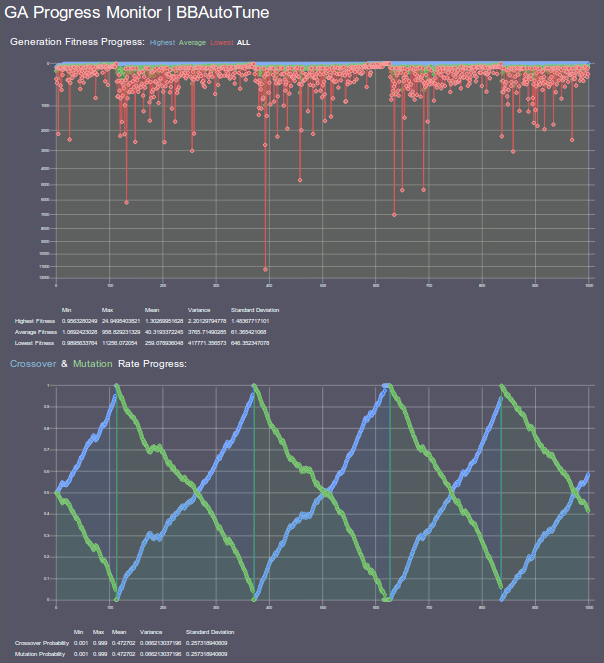
\includegraphics[scale=0.6]{../Figures/Chapter4/ga_monitor.png}
\rule{35em}{0.5pt}
\caption[GA Progress Monitor]{Here you see external GA progress monitor.}
\label{fig:ga_monitor}
\end{figure}

\subsection{Genetic Algorithm}

The genetic algorithm for BBAutoTune was borrowed from the SimPL project and ported to Python with some aspects of the GA being altered to suit the needs of BBAutoTune. Since lower values of fitness are considered higher than those of higher values of fitness, the population sorting function needed to be altered. Other portions altered were the selection operator, the population metrics calculator, and the self-adaptation algorithm.  

\subsubsection{Encoding Scheme}

The physics parameters selected for tuning were a mixed set of floats, integers, string arrays, and boolean values. To ease the process of crossover and mutation, all genome genes were homogenized to a normalized range of $[0.0,1.0]$. Let any given genome's gene value be $g_i$ and any given physics parameter be $p_i$. For a float type with a maximum range value $r_{max}$ and minimum range value $r_{min}$, the mapping function was $p_i=(g_i*(r_{max}-r_{min}))+r_{min}$. For an integer type with a maximum range value $r_{max}$ and a minimum range value $r_{min}$, the mapping function was $p_i=\lfloor(g_i*(r_{max}-r_{min}))+r_{min}\rfloor$. For an array $A$ of strings type with size $n$, the mapping function was $p_i=A[\lfloor g_i*(n-1)\rfloor]$. Finally for a boolean type, the mapping function was 

\[ p_i = \left\{
\begin{array}{l l}
True & \quad \text{if $g_i\geq 0.5$,}\\
False & \quad \text{if $g_i < 0.5$.}
\end{array} 
\right.\]

\subsubsection{Operators}

The operators used include selection, elitism, crossover, and mutation. All of these operators work together to generate a new population once the current population has been fully evaluated by the fitness function.

The selection operator includes two variants: tournament selection and rank fitness selection. The user can indicate on the GUI panel if rank fitness selection is to be used---otherwise tournament selection will be used. Tournament selection works by gathering a sub-portion of the total population where the fittest genome among the sub-portion is selected thereby winning the tournament \cite{Miller95geneticalgorithms}. While gathering the sub-portion, all genomes in the population have a uniform probability of being included in the tournament regardless of their respective fitness values. There is the possibility that the same genome may be included in the tournament more than once. For crossover, two tournaments of size three are run thereby giving two genomes to be crossed. For mutation, one tournament of size two is run thereby giving one genome to be mutated. Rank fitness selection works by first sorting the population in non-increasing order according to fitness and then selects a genome at random where the probability of a genome being selected is proportional to its rank fitness. With the population in sorted order, the first genome is given a rank fitness of 1, the second genome is given a rank fitness of 2, ..., and the last genome is given a rank fitness of $n$ which is the population size. The rank fitness prefix-sum for each genome is calculated in an array such that the first index value in the prefix-sum array is $1$ while the last index value in the prefix-sum array is $\frac{n(n-1)}{2}$. A uniform random number is selected in the range $\left[0,\frac{n(n-1)}{2}\right]$. The genome selected $G$ is the one in which the random number is greater than the previous prefix-sum for genome $G_{i-1}$ and less than or equal to the prefix-sum for $G_i$. Genomes with a higher fitness will have a higher rank fitness and thus will have a higher probability of being selected for either crossover or mutation. See Figure \ref{fig:rank_fitness_selection}. 

\renewcommand{\baselinestretch}{1.0}

\begin{figure}[htbp]
\begin{center}
\begin{varwidth}{\textwidth}
{\tt
BEGIN \\
\tab Population $P$ with size $n$ has been evaluated \\
\tab Sort $P$ in non-increasing order \\
\tab For i=1 to $n$ do \\
\tab \tab $P[i-1].rankFitness = i$ \\
\tab End for \\
\tab For i=0 to $n-1$ do \\
\tab \tab $P[i].prefixSum = \sum\limits_{k=0}^i(P[k].rankFitness)$ \\
\tab End for \\
\tab Select a random number $r=unif\left(0,\frac{n(n-1)}{2}\right)$ \\
\tab Genome selected $G$ \\
\tab For i=0 to $n-1$ do \\
\tab \tab If $P[i].prefixSum \geq r $ then \\
\tab \tab \tab $G=P[i]$ \\
\tab \tab \tab Break \\
\tab \tab End if \\
\tab End for \\
\tab Return $G$ \\
END \\
}
\end{varwidth}
\end{center}
\centering
\rule{35em}{0.5pt}
\caption[Rank Fitness Selection Algorithm]{Here you see the rank fitness selection algorithm.}
\label{fig:rank_fitness_selection}
\end{figure}

\subsubsection{Fitness Function}

%\todo{This section only reflects the data recorded using the old move() function. Change to reflect data collected using the new motion() function.}

To construct the fitness function, real robot motion data was collected which included 1040 sample points. X-translation, y-translation, and z-rotation were recorded for the real robot. With a camera overhead, the real robot was place in the arena and was repeatedly commanded to go forward (relative from its current position and orientation) 25 centimeters. Care was taken to avoid having the robot collide with the arena walls. Once the robot consecutively moved forward three times, the robot rotated in place by 135 degrees and was not recorded during this period of rotation.  

Using the camera, the robot's position and orientation before and after performing the forward command was recorded for each forward command issued. The robot's position and orientation was not reset each time the robot performed a forward command. Instead, the robot was allowed to continue forward from its current position and orientation as it traveled around the arena. Thus each recorded pair of initial and final states were translated and rotated to be in the same reference frame such that the robot was always at the arena origin facing down the positive x-axis before performing the forward command. See Figure \ref{fig:real_robot_raw_trans_rot} and \ref{fig:real_robot_forward_motion}. Note that from the robot's perspective, it is always facing down its local positive x-axis no matter its position or orientation as seen from some other reference point.

\begin{figure}[htbp]
\centering
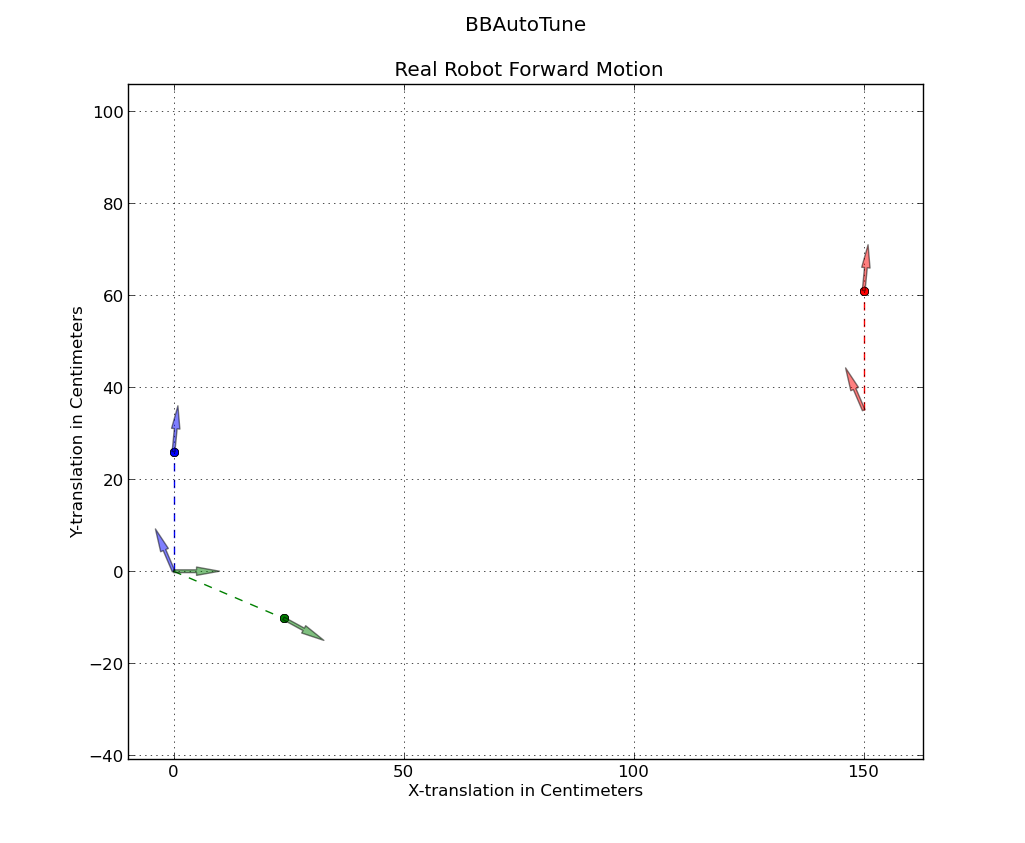
\includegraphics[scale=0.6]{../Figures/Chapter4/real_robot_raw_trans_rot.png}
\rule{35em}{0.5pt}
\caption[Real Robot Forward Motion Data Translated and Rotated Example]{Here you see a specific instance of how the raw real robot forward motion data was translated and rotated such that each pair of initial and final states have the same reference frame. The red arrows, dot, and line represent the raw initial and final state of the robot recorded from the overhead camera before and after it performed the forward command. The blue arrows, dot, and line represent the initial and final state translated to the origin. The green arrows, dot, and line represent the initial and final state rotated by the amount needed to align the initial orientation with the positive x-axis. For each colored group, the dot and arrow pair represent the position and orientation of the robot after having performed the forward command while the arrow without a dot represents the position and orientation state of the robot before it performed the forward command.}
\label{fig:real_robot_raw_trans_rot}
\end{figure}

\begin{figure}[htbp]
\centering
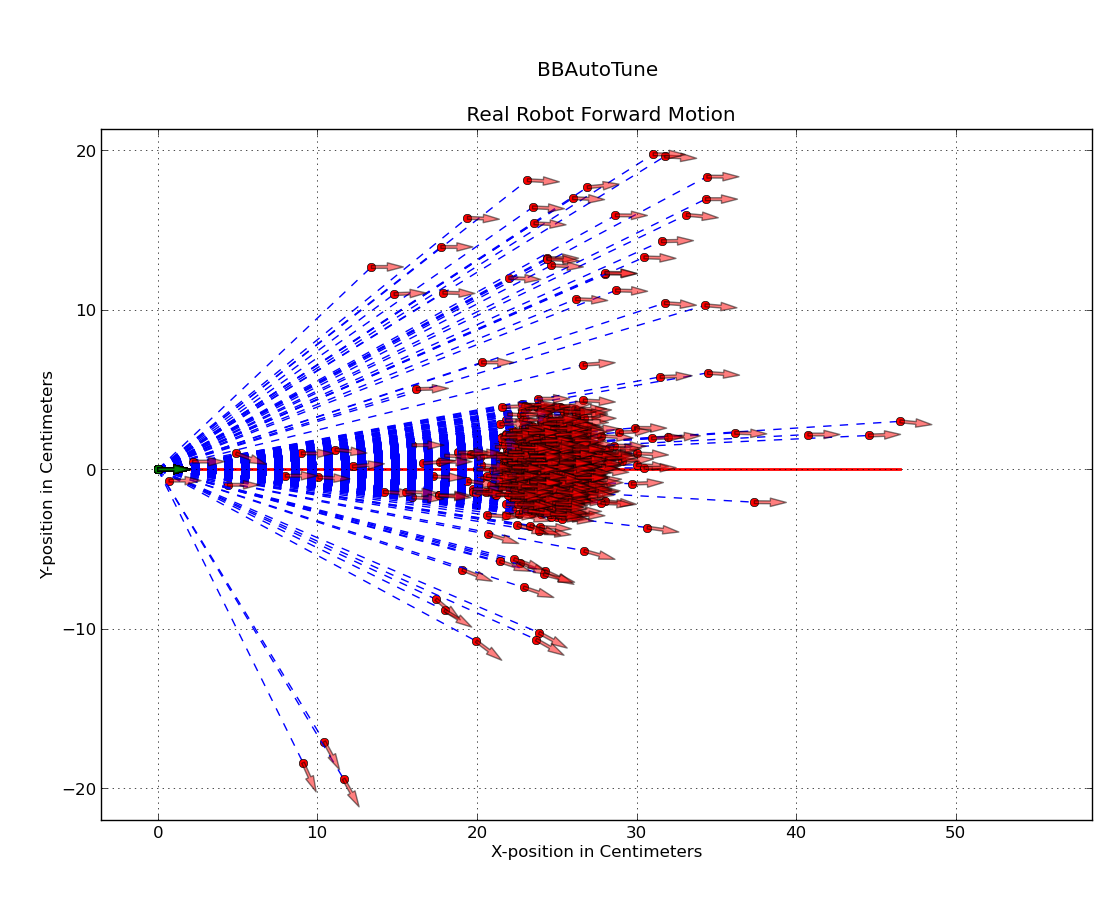
\includegraphics[scale=0.6]{../Figures/Chapter4/real_robot_forward_motion.png}
\rule{35em}{0.5pt}
\caption[Real Robot Forward Motion]{Here you see the collected real robot forward motion plotted from the same reference point. The green dots and arrows indicate the starting position and orientation of the real robot before the forward command was performed. The red dots and arrows indicate the ending position and orientation of the real robot after the forward command was performed. The dots represent position and the arrows represent orientation. The broken blue lines connect the initial states to their corresponding finals states.}
\label{fig:real_robot_forward_motion}
\end{figure}

Analyzing the distribution of x-translation, y-translation, and z-rotation separately, all are unimodal and nearly symmetric with only a slight skew from their respective means. See Table \ref{tab:real_robot_motion_dist} and Figure \ref{fig:real_robot_forward_dist}. When viewing the change in dimensions together, a large mass is centered around the point: 23.8644631679cm, 0.338269853117cm, and -0.00417473025048rad. See Figure \ref{fig:real_robot_3d_scatter}. Based on the variance-covariance matrix, all three dimensions vary together and are not independent from one another. % \todo{Citation needed?} 

\begin{table}[htbp]
\centering
\footnotesize
\bgroup
\def\arraystretch{1.1}
\begin{tabular}{ | >{\centering\arraybackslash}m{3cm} | >{\centering\arraybackslash}m{3cm} | >{\centering\arraybackslash}m{3cm} | >{\centering\arraybackslash}m{3cm} | }
%\hline
%\rowcolor{gray}
\cline{2-4}
\multicolumn{1}{c|}{}                  & \cellcolor{gray} X-translation & \cellcolor{gray} Y-translation & \cellcolor{gray} Z-rotation \\ \hline
\cellcolor{gray} Max                   & 46.5183415482cm        & 19.7486813209cm       & 6.23776rad           \\ \hline
\cellcolor{gray} Min                   & 0.0cm                  & -19.4028539247cm      & -1.148163rad         \\ \hline
\cellcolor{gray} Mean/Centroid         & 23.8644631679cm        & 0.338269853117cm      & -0.00417473025048rad \\ \hline
\cellcolor{gray} Mode                  & 25.0cm                 & -1.0cm                & 0.0rad               \\ \hline
\cellcolor{gray} Variance              & 10.3960320996          & 9.46441502772         & 0.152467827567       \\ \hline
\cellcolor{gray} Standard Deviation    & 3.22428784378          & 3.07642894079         & 0.390471289043       \\ \hline
\cellcolor{gray} Covariance with X-translation  & 10.4060572             & 2.3348963             & 0.0685591            \\ \hline
\cellcolor{gray} Covariance with Y-translation  & 2.3348963              & 9.47354175            & 0.08654865           \\ \hline
\cellcolor{gray} Covariance with Z-rotation     & 0.0685591              & 0.08654865            & 0.15261486           \\ \hline
\end{tabular}
\egroup
\caption[Real Robot Forward Motion Distribution Metrics]{Here you see the distribution metrics for surge, sway, and yaw.}
\label{tab:real_robot_motion_dist}
\end{table}

% Number of sample points:  1040
% X' max/min:  46.5183415482 0.0
% X' mode:  (array([ 25.]), array([ 8.]))
% X' mean:  23.8644631679
% X' variance:  10.3960320996
% X' standard deviation:  3.22428784378
% Y' max/min:  19.7486813209 -19.4028539247
% Y' mode:  (array([-1.]), array([ 8.]))
% Y' mean:  0.338269853117
% Y' variance:  9.46441502772
% Y' standard deviation:  3.07642894079
% Theta' max/min:  6.23776 -1.148163
% Theta' mode:  (array([ 0.]), array([ 234.]))
% Theta' mean:  -0.00417473025048
% Theta' variance:  0.152467827567
% Theta' standard deviation:  0.390471289043
% X' normal test p-value:  2.45603600615e-124 Not Normal
% Y' normal test p-value:  1.60589004385e-121 Not Normal
% T' normal test p-value:  0.0 Not Normal
% Covariance matrix: 
% [[ 10.4060572    2.3348963    0.0685591 ]
%  [  2.3348963    9.47354175   0.08654865]
%  [  0.0685591    0.08654865   0.15261486]]
% X', Y', T' Median:  24.0201969119 ,  0.0475373929135 ,  -0.0145985
% X'Y'T' Centroid:  23.8644631679 ,  0.338269853117 ,  -0.00417473025048
% X'Y'T' Geometric Median:  23.9754618867 ,  0.0401244563225 ,  -0.0124671288475

\begin{figure}[htbp]
\centering
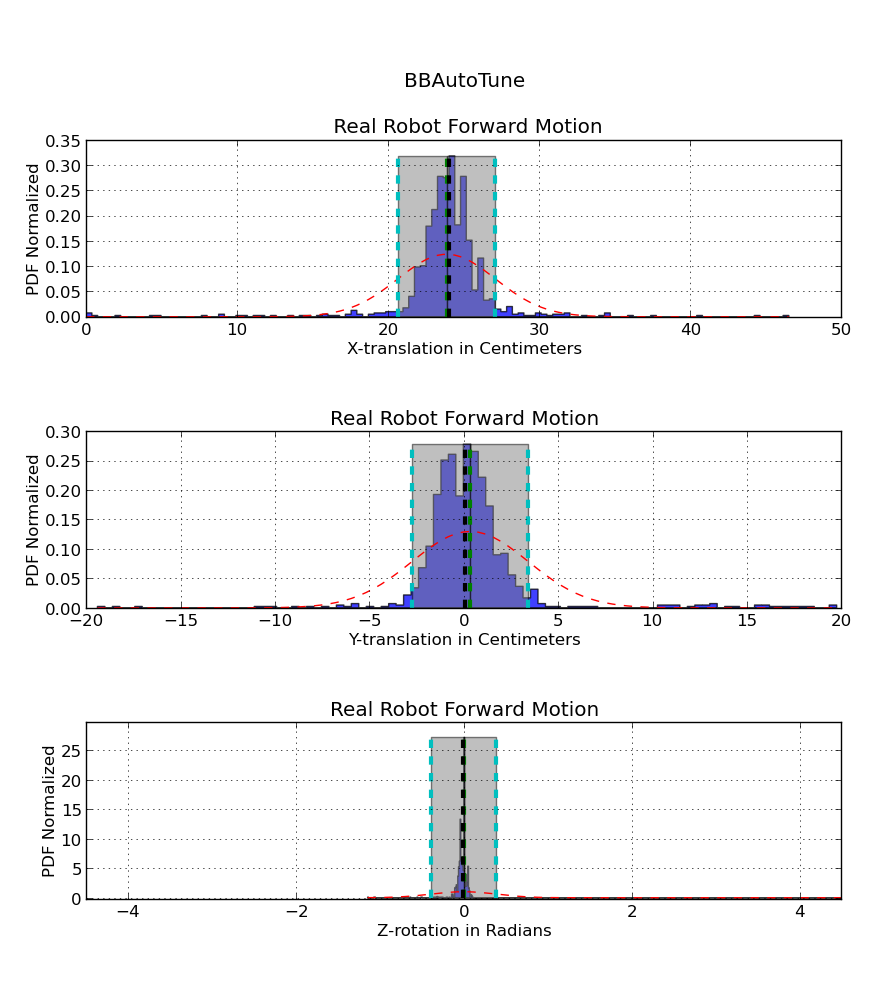
\includegraphics[scale=0.6]{../Figures/Chapter4/real_robot_forward_dist.png}
\rule{35em}{0.5pt}
\caption[Real Robot Forward Motion Distributions]{Here you see the distribution of x-translation, y-translation, and z-rotation dimensions recorded for the real robot forward motion. The broken black bar represents the mode, the green broken bar represents the mean, the cyan broken bars represent one standard deviation from the mean, and the red broken curve represents the best fit normal curve.}
\label{fig:real_robot_forward_dist}
\end{figure}

\begin{figure}[htbp]
\centering
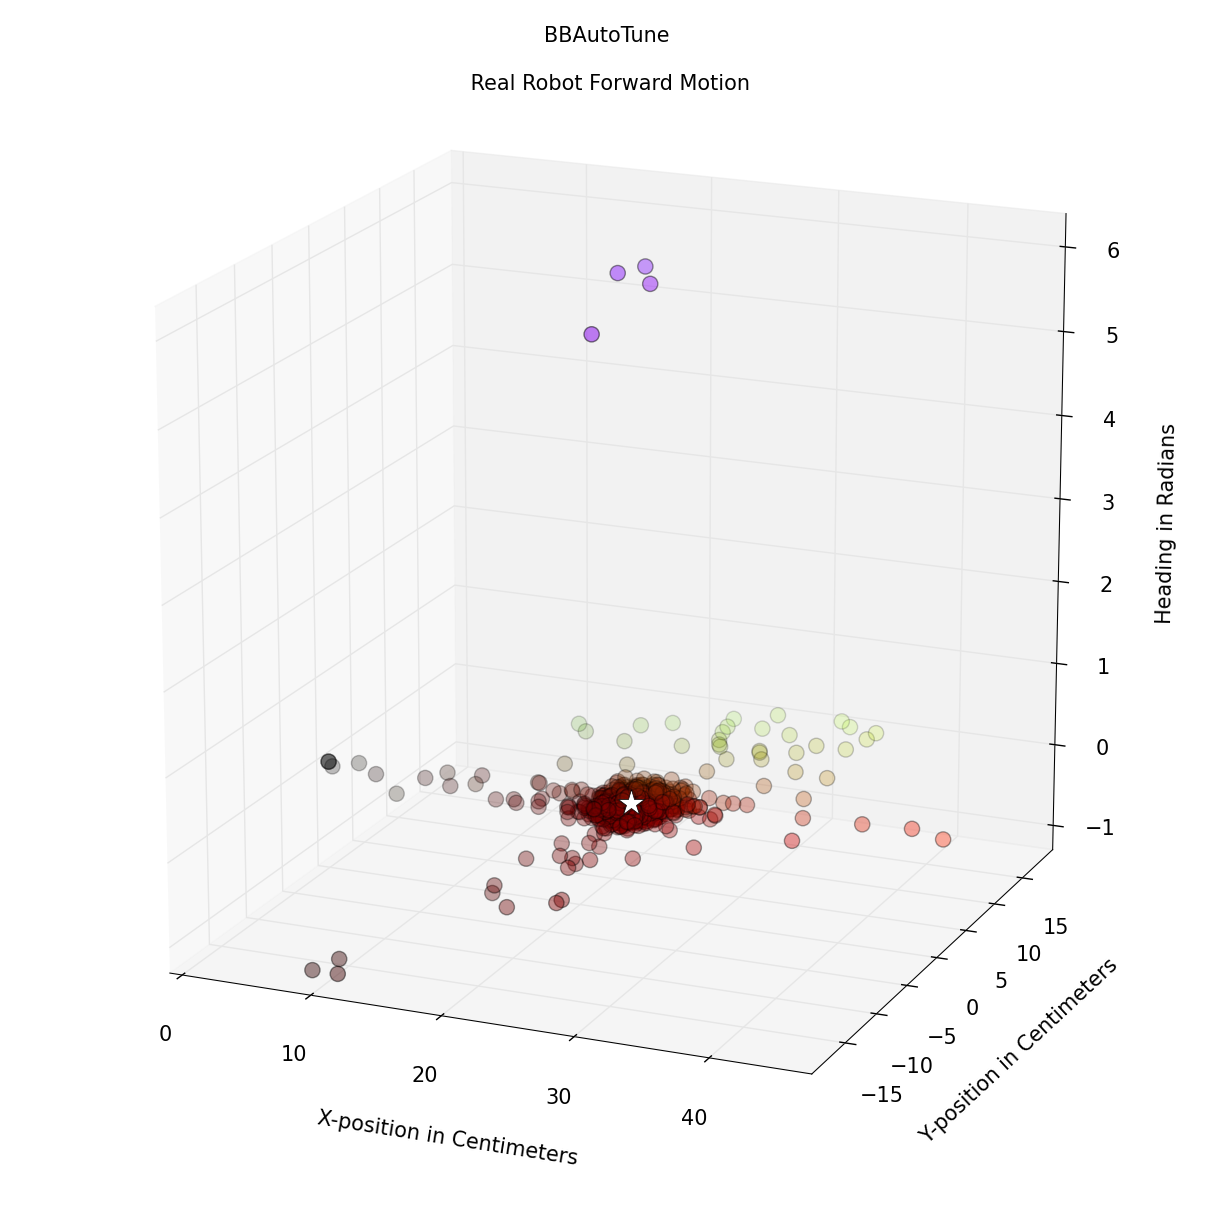
\includegraphics[scale=0.5]{../Figures/Chapter4/real_robot_3d_scatter.png}
\rule{35em}{0.5pt}
\caption[Real Robot Forward Motion 3D Scatter Plot]{Here you see a 3D scatter plot of the x-translation, y-translation, and z-rotation values for the real robot after it performed the forward command. Positive values of x-translation, y-translation, and z-rotation contribute a portion of red, green, and blue respectively to each scatter plot. The star located at the center of the large mass of points is the centroid.}
\label{fig:real_robot_3d_scatter}
\end{figure}

With the real robot motion data collected and analyzed, a metric was needed for the fitness function. This metric would need to indicate how different or dissimilar the movement of the simulated robot was from the real robot while running the GA. The intuition was that as the simulated robot motion observed moved closer to the centroid of the real robot motion, the simulated motion would become increasingly indistinguishable from the real motion. Various distance functions were looked at and the Mahalanobis distance was chosen as the basis for the fitness function. The Mahalanobis distance is the generalized form of the Euclidean distance such that the Mahalanobis distance accounts for the correlation in the data set since it is computed using the inverse of the variance-covariance matrix \cite{mahalanobis_distance}. For uncorrelated data, the Mahalanobis distance reduces to the Euclidean distance \cite{what_is_mahalanobis_distance}.

Inefficiencies with the overhead camera and the timing at which the position and orientation state of the real robot was captured could have potentially skewed the real robot motion model with outliers ultimately resulting in a skewed multivariate mean location and a skewed inverse variance-covariance matrix making the Mahalanobis distance skewed. To account for the potential outliers in the real motion data set, a robust mean location and a robust variance-covariance matrix was computed from the data set using the Fast-MCD algorithm implemented in the Scikit-learn Python module \cite{Rousseeuw:1999:FAM:331435.331458}\cite{scikit-learn}. The classical mean location was 23.8644632cm, 0.338269853cm, and -0.00417473025rad for x-translation, y-translation, and z-rotation respectively while the robust mean location was 23.9934044cm, 0.0351240536cm, and -0.0189964938rad for x-translation, y-translation, and z-rotation respectively. The left matrix below was the classical variance-covariance matrix while on the right was the robust variance-covariance matrix returned by the Fast-MCD algorithm.
\vspace{-1mm}
\[ \left( \begin{array}{ccc}
10.3960321 &  2.33264688 & 0.06849305 \\
2.33264688 &  9.46441503 & 0.08646527 \\
0.06849305 &  0.08646527 & 0.15246783 \\
\end{array} \right)
%
\left( \begin{array}{ccc}
1.46298445 & 0.13924542 & 0.00223493 \\
0.13924542 & 1.64197605 & 0.0168499  \\
0.00223493 & 0.0168499  & 0.00173777 \\
\end{array} \right)
\]

\noindent
The resulting samples weighted higher than others by the Fast-MCD algorithm are shown in Figure \ref{fig:robust_support_samples}. These samples where used to calculate the robust mean and the robust variance-covariance matrix returned by the algorithm. By substituting the robust mean and the inverse of the robust variance-covariance matrix into the Mahalanobis distance calculation, the robust distance $RD$ for any sample point can be computed \cite{WICS:WICS61}. Comparisons between the Mahalanobis distance and the robust distance for each of the 1040 real robot motion data points are shown in Figure \ref{fig:real_robot_md_vs_rd}. As the data points travel away from the centroid, the robust distance increases more rapidly than the Mahalanobis distance.  

% Classical Mean (Location):  [  2.38644632e+01   3.38269853e-01  -4.17473025e-03]
% Robust Mean (Location):  [  2.39934044e+01   3.51240536e-02  -1.89964938e-02]
% Classical Covariance Matrix: 
% [[ 10.3960321    2.33264688   0.06849305]
%  [  2.33264688   9.46441503   0.08646527]
%  [  0.06849305   0.08646527   0.15246783]]
% Robust Covariance Matrix: 
% [[ 1.46298445  0.13924542  0.00223493]
%  [ 0.13924542  1.64197605  0.0168499 ]
%  [ 0.00223493  0.0168499   0.00173777]]   

\begin{figure}[htbp]
\centering
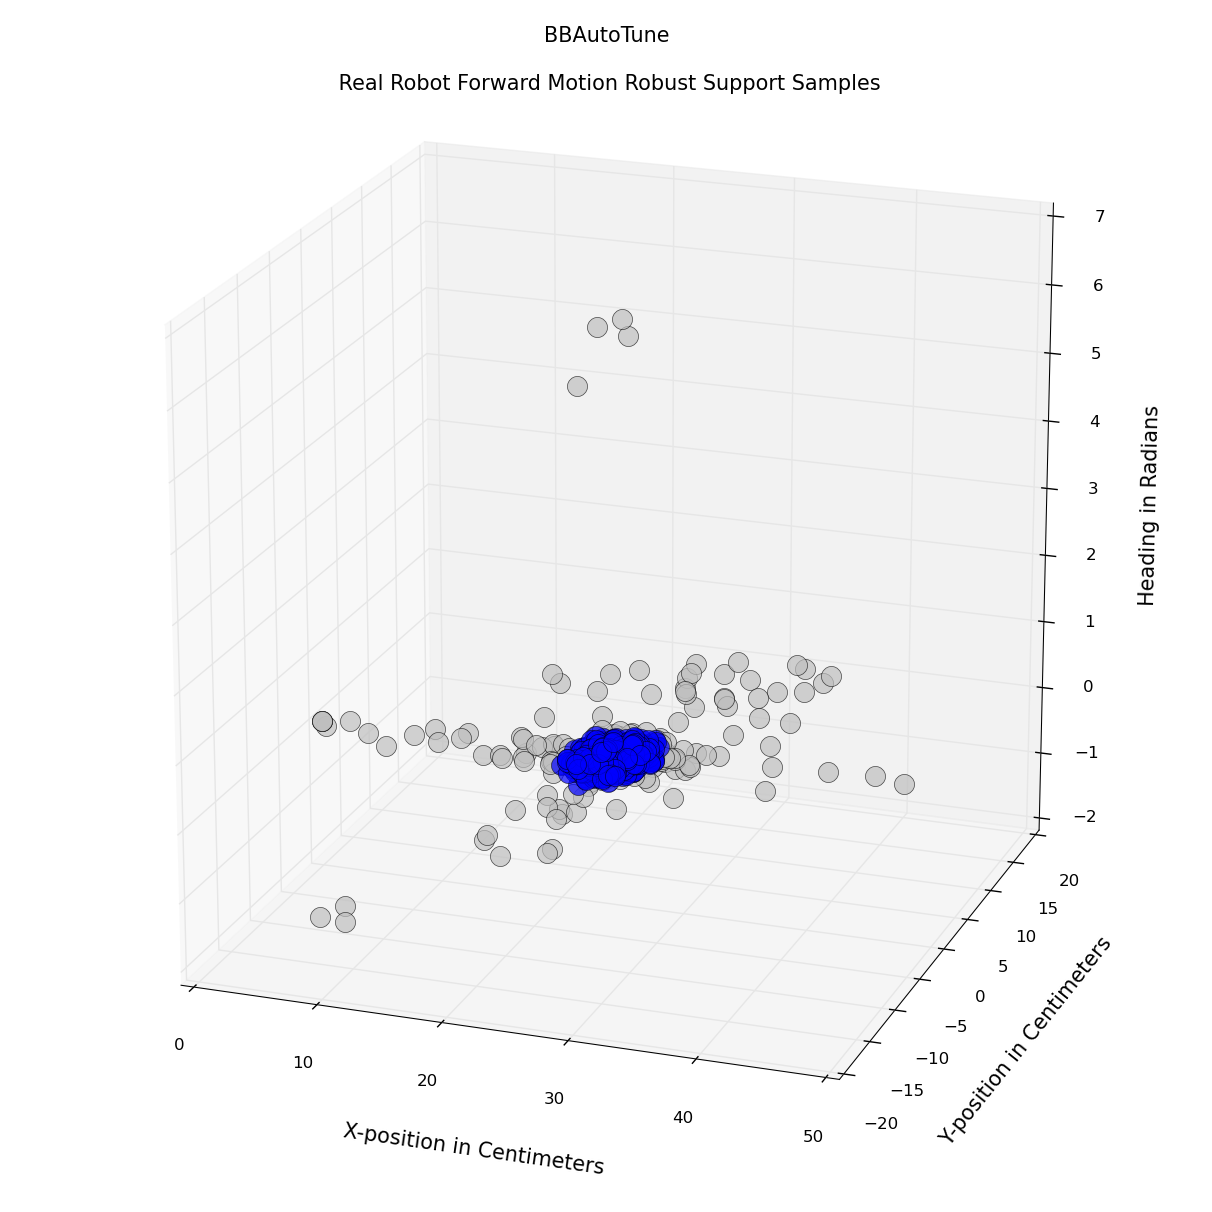
\includegraphics[scale=0.5]{../Figures/Chapter4/real_robot_robust_samples.png}
\rule{35em}{0.5pt}
\caption[Real Robot Forward Motion Fast-MCD Support Samples]{Here you see a 3D scatter plot of the support samples in blue used to calculate the robust mean location and the robust variance-covariance matrix as returned by the Fast-MCD algorithm.}
\label{fig:robust_support_samples}
\end{figure}

\begin{figure}[htbp]
\centering
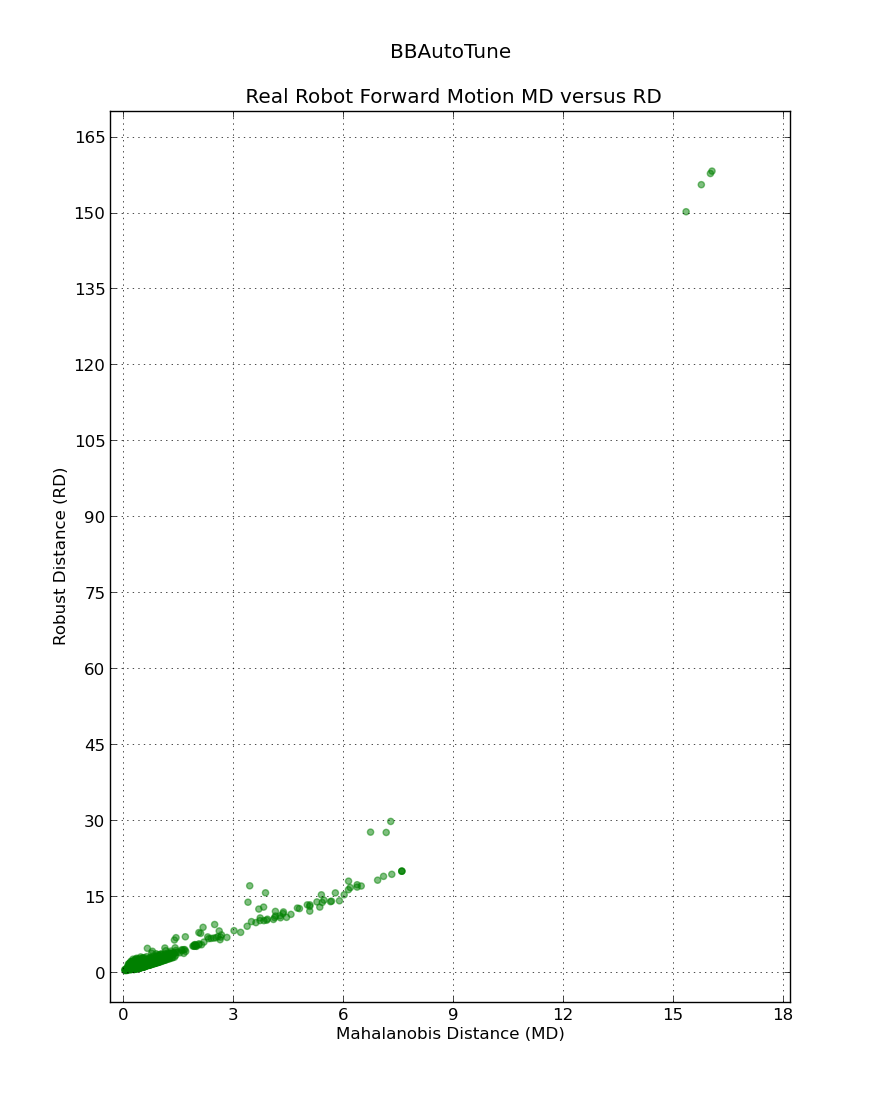
\includegraphics[scale=0.5]{../Figures/Chapter4/real_robot_md_vs_rd.png}
\rule{35em}{0.5pt}
\caption[Real Robot Forward Motion MD versus RD]{Here you see a scatter plot comparing the Mahalanobis distance versus the robust distance for each data point collected of the real robot motion.}
\label{fig:real_robot_md_vs_rd}
\end{figure}

Only three out of the total six degrees of freedom were recorded for the real robot. However, in Blender there were an additional three degrees (pitch, roll, and heave) to contend with.  Thus, the simulated-robot base's x-rotation, y-rotation, and z-translation were constrained. Additionally, all wheels had their z-translation constrained. As an added precaution, penalties where added onto the robust distance by the absolute amount the simulated robot's base violated x-rotation, y-rotation, and/or z-translation. Additionally, a time penalty was added onto the robust distance by the amount of time in seconds the simulated robot took to evaluate greater than one second with a max penalty of 15 seconds since any given evaluation period only lasted a total of 16 seconds.

Once the simulated robot was run through the game engine evaluation period (using the physics parameter settings decoded from the currently being evaluated genome $G_i$'s genes), 14 pieces of data was collected by the robot monitor for use in the fitness function. Let $S=[x_t,y_t,z_t,x_r,y_r,z_r,t]$ be the starting state of the simulated robot at the beginning of the evaluation period at time $S[6]=t$ where the subscript $_t$ refers to translation and the subscript $_r$ refers to rotation. Let $S'=[x_t,y_t,z_t,x_r,y_r,z_r,t]$ be the ending state of the simulated robot at the end of the evaluation period at time $S'[6]=t$. Also, let $RD(x-translation,y-translation,z-rotation)$ be the robust distance. The fitness function and thus the fitness of $G_i$ was defined as $Fitness(S,S')=RD(S'[0]-S[0],S'[1]-S[1],S'[5]-S[5])+|S'[4]-S[4]|+|S'[3]-S[3]|+|S'[2]-S[2]|+((S'[6]-S[6])-1)=G_i$'s fitness. The range of this function is $[0,\infty)$. Since the goal of this thesis was to have the simulated robot move as the real robot, the desired output of this function was $0.0$ implying that three objectives were met:
\begin{itemize}
 \item The simulated robot's x-translation, y-translation, and z-rotation after moving was 23.9934044cm, 0.0351240536cm, and -0.0189964938rad respectively.
 \item The simulated robot stopped moving after one second.
 \item The simulated robot did not fall through the floor, flip over, roll over, and/or launch upward.
\end{itemize}
Thus the goal of the GA was to minimize this function whereby lower output values were a higher fitness than higher output values.

\subsubsection{Evaluation Setup}

For each evaluation period (the running of the game engine), the 3D robot model's local coordinate system was axis aligned with the world coordinate system, the robot was faced forward looking down the positive x-axis, and its local origin was placed at the world origin. See Figure \ref{fig:simu_robot_aligned}. Before each evaluation period, the physics engine parameters were set to the values decoded from the genes of the currently being evaluated genome. All evaluation periods lasted no more than 16 seconds. If the robot stopped moving before 16 seconds, then the evaluation period ended immediately. The only applied force to the robot was the wheel torque where each wheel received the same amount of applied torque for the same duration. The duration of applied torque was roughly 16 milliseconds after which no further force was applied to the robot.

\begin{figure}[htbp]
\centering
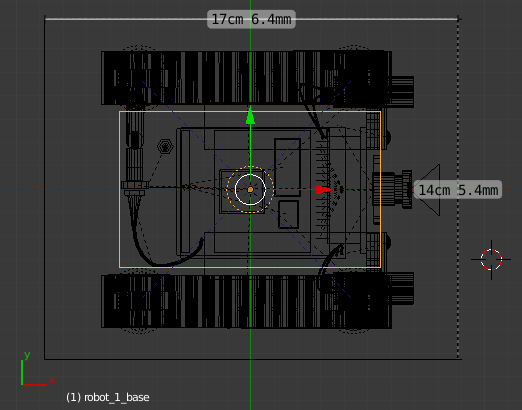
\includegraphics[scale=0.5]{../Figures/Chapter4/simu_robot_aligned.png}
\rule{35em}{0.5pt}
\caption[Simulated Robot Axis Aligned]{Here you see the simulated robot's local coordinate system axis aligned with the world coordinate system.}
\label{fig:simu_robot_aligned}
\end{figure}

\section{Platform}

For all experiments, BBAutoTune was run on a 64bit Linux operating system with 32GB of RAM and an Intel Core i7-4770K four core processor running at 3.9GHz.

\section{Experimental Designs}

The purpose for experiment one was to determine a base set of physics parameters that have significant influences over the physics simulation. Experiments two through five involved actually tuning the physics engine and comparing the simulated versus real robot motion. Self-adaptation and tournament versus rank fitness selection were the experimental GA parameters for experiments two through five. 

\subsection[Experiment One]{Experiment one: physics engine parameter influence.}

The potential Blender physics engine parameter candidates---to be tuned by the GA---were analyzed for their influence over the physics simulation. To accomplish this goal, a racquetball like environment was constructed in Blender which consisted of a ball, an enclosed arena, and an automated racket controlled via a Python script. See Figure \ref{fig:racquetball}. Note that the ball was allowed to travel in all three dimensions and was completely physics based.

\begin{figure}[htbp]
\centering
\includegraphics[scale=0.4]{../Figures/Chapter4/racquetball.png}
\rule{35em}{0.5pt}
\caption[Physics Engine Parameter Influence Racquetball Environment]{Here you see the racquetball environment used to test the physics engine parameter candidates' influence over the physics simulation.}
\label{fig:racquetball}
\end{figure}

44 candidate parameters were selected for testing in the racquetball environment. All parameters tested were only associated with the ball. Before all of these parameters were tested for their influence, \textit{nice} values were selected for each such that the ball's behavior was visually normal. A standard was established where the ball was allowed to run for five seconds (with all parameters being set to their nice values) during which its location was recorded at roughly 60 times per second. With the standard established---with which all other runs would be compared to---a parameter was selected (from the candidate pool), its value was tweaked, the ball was run for five seconds with its location being recorded at roughly 60 times per second, and after the run was over, the tweaked parameter's value was set back to its nice value. This sequence was repeated for all 44 candidate parameters.

\subsection[Experiment Two]{Experiment two: tournament selection with self-adaptation.}

Very early runs of BBAutoTune attempted to tune physics parameters: gravity, sub-steps, FPS, use material physics, material friction, material elasticity, mass, form factor, velocity maximum, damping translation, damping rotation, use collision bounds, collision bound type, and torque where the search space for each parameter was its entire valid range. This proved to be problematic since some of the valid ranges are quite large especially torque with a max upper bound of $~3.40\times10^{38}$. While running the game engine, if the genome's genes decoded to relatively high physics engine parameter values, world coordinates would return the Python values ``NaN'' or ``inf''.

To rectify this issue, the set of physics parameters selected for tuning was pruned and for the parameters left, their ranges were shortened to reasonable upper and lower bounds found manually. The resulting set of tunable physics parameters and their ranges for experiment two were: gravity [0.0,15.0], sub-steps [1,5], FPS [30,10000], material friction [0.0,100.0], material elasticity [0.0,1.0], mass [0.010,15.0], velocity maximum [0.0,1000.0], damping translation [0.0,1.0], damping rotation [0.0,1.0], collision bound type [TRIANGLE\_MESH,CONVEX\_HULL,CYLINDER,SPHERE], and torque [0.0,100.0]. Use material physics and use collision bounds were set to true and held constant. Form factor was set to 1.0 and was held constant. 

The GA was run for 500 generations, tournament selection was used, the population size was set to 10, elitism was set to 2, crossover and mutation were performed separately, and the crossover and mutation probabilities were self-adapted over time.

\subsection[Experiment Three]{Experiment three: tournament selection without self-adaptation.}

The set of tunable physics parameters for experiment three was the same as experiment two. The GA was run for 500 generations, tournament selection was used, the population size was set to 10, elitism was set to 2, crossover and mutation were performed separately, and the crossover and mutation probabilities were held constant at 0.8 and 0.2 respectively.

\subsection[Experiment Four]{Experiment four: rank fitness selection with self-adaptation.}

The set of tunable physics parameters for experiment four was the same as experiment two. The GA was run for 500 generations, rank fitness selection was used, the population size was set to 10, elitism was set to 2, crossover and mutation were performed separately, and the crossover and mutation probabilities were self-adapted over time.

\subsection[Experiment Five]{Experiment five: rank fitness selection without self-adaptation.}

The set of tunable physics parameters for experiment five was the same as experiment two. The GA was run for 500 generations, rank fitness selection was used, the population size was set to 10, elitism was set to 2, crossover and mutation were performed separately, and the crossover and mutation probabilities were held constant at 0.8 and 0.2 respectively.

\section{Experimental Results}

Experiment two had the highest performing genome out of experiments two through five. Experiments three through five had similar highest fitnesses. Using self-adaptation with tournament selection resulted in the highest fitness observed among experiments two through five. Comparing experiment two to three, self-adaptation was beneficial but was not beneficial when comparing experiment five to four.   

\subsection[Experiment One]{Experiment one: physics engine parameter influence.}

To compare the recorded tweaked-parameter ball paths with the recorded standard, four methods were utilized to give an indication as to how much influence any one candidate parameter had over the simulation. The first method was visual inspection. All 44 tweaked-parameter ball paths were plotted against the standard. See Figure \ref{fig:matphysplot} and Figure \ref{fig:logicstepsplot}. The second method was an in-house algorithm, titled the \textit{Lettier distance}, which gives the maximum euclidean distance between two discrete curves $P$ and $Q$. Informally, imagine holding a rubber band in your hands where the left hand affixes the left end of the rubber band to the first point in $P$ and the right hand affixes the right end of the rubber band to the first point in $Q$. During each iteration, you advance the left end of the rubber band to the next point in $P$ and you advance the right end of the rubber band to the next point in $Q$. If the distance grows between point $p_i\in P$ and point $q_j \in Q$, the rubber band stretches but never shrinks. If $|P|<|Q|$ then you hold the left end of the rubber band to the last point in $P$ and continue advancing to the last point in $Q$ and vice versa. Once you reach the last point in $P$ and the last point in $Q$, the resulting length of the rubber band is the max euclidean distance between $P$ and $Q$. See Figure \ref{lettierdistance}. The third method was the discrete Fr{\'e}chet distance and the fourth method was the Hausdorff distance \cite{frechet} \cite{hausdorff}.

\begin{figure}[htbp]
\centering
\includegraphics[scale=0.35]{../Figures/Chapter4/material_physics_ball_plot.png}
\rule{35em}{0.5pt}
\caption[Physics Engine Racquetball Path Dissimilarity]{Here you see the dissimilarity of the ball paths between the tweaked, material-physics elasticity parameter and the standard (where no parameters were tweaked).}
\label{fig:matphysplot}
\end{figure}

\begin{figure}[htbp]
\centering
\includegraphics[scale=0.35]{../Figures/Chapter4/logic_steps_ball_plot.png}
\rule{35em}{0.5pt}
\caption[Physics Engine Racquetball Path Similarity]{Here you see the similarity of the ball paths between the tweaked, logic-steps max parameter and the standard (where no parameters were tweaked).}
\label{fig:logicstepsplot}
\end{figure}

\begin{figure}[htbp]
\begin{center}
\begin{varwidth}{\textwidth}
{\tt
BEGIN \\
\tab $P = \langle p_1, p_2,...,p_n\rangle$ \\
\tab $Q = \langle q_1, q_2,...,q_m\rangle$ \\
\tab $max = 0.0$ \\
\tab For all $p_i\in P$ and $q_j \in Q$ do \\
\tab \tab $d = ||p_i-q_j||$ \\
\tab \tab If $max$ $<$ $d$ then \\
\tab \tab \tab $max=d$ \\
\tab \tab End if \\
\tab End for \\
\tab Return $max$ \\
END \\
}
\end{varwidth}
\end{center}
\centering
% \begin{equation*}
% \begin{align}
% Algorithm: & \\
% & P = \langle p_1, p_2,...,p_n\rangle \\
% & Q = \langle q_1, q_2,...,q_m\rangle \\
% & max = 0.0 \\
% & For \ all \ p_i\in P \ and \ q_j \in Q \ do: \\
% & \quad d = ||p_i-q_j|| \\
% & \quad If \ max < d \ then: \\
% & \qquad max \leftarrow d \\
% & return \ max \\
% \end{align}
% \end{equation*}
\rule{35em}{0.5pt}
\caption[Lettier Distance Algorithm]{Here you see the Lettier distance algorithm.}
\label{lettierdistance}
\end{figure}

20 parameters out of the initial 44 showed no significant influence over the 3D physics simulation in Blender. Thus, the resulting 24 parameters which did have a significant influence were targeted for tuning by the genetic algorithm. See Table \ref{tab:distances}.

\begin{table}[htbp]
\centering
\footnotesize
\def\arraystretch{1.1}
\begin{tabular}{ | l || l | l | l | }
\hline
\rowcolor{gray}
Tweaked Parameter: Value & Lettier Distance & Discrete Fr{\'e}chet Distance & Hausdorff Distance \\ \hline
Gravity: $1.0\frac{m}{s^2}$ & 12.7741189989 & 20.948159542 & 9.86343687719 \\ \hline
\rowcolor{cyan}
Physics Steps Max: 1 & 0.329232644023 & 0.329232644023 & 0.329232644023 \\ \hline
Physics Sub-steps: 50 & 19.3073641073 & 17.0708640308 & 11.3180046289 \\ \hline
Physics FPS: 1 & 218.037284056 & 211.287842927 & 205.848670021 \\ \hline
\rowcolor{cyan}
Logic Steps Max: 1 & 0.329232644023 & 0.329232644023 & 0.329232644023 \\ \hline
\rowcolor{cyan}
Physics Deactivation Linear Threshold: 10000.0 & 0.329232644023 & 0.329232644023 & 0.329232644023 \\ \hline
\rowcolor{cyan}
Physics Deactivation Angular Threshold: 10000.0 & 0.329232644023 & 0.329232644023 & 0.329232644023 \\ \hline
\rowcolor{cyan}
Physics Deactivation Time: 0.0 & 0.329232644023 & 0.329232644023 & 0.329232644023 \\ \hline
\rowcolor{cyan}
Occlusion Culling: False & 0.329232644023 & 0.329232644023 & 0.329232644023 \\ \hline
\rowcolor{cyan}
Occlusion Culling Resolution: 1024 & 0.329232644023  & 0.329232644023  & 0.329232644023 \\ \hline
Material Physics: False & 18.0830473811 & 18.0830473811  & 18.0830473811 \\ \hline
Material Physics Friction: 100.00 & 4.93924881608  & 4.94095279557  & 3.8109066203 \\ \hline
Material Physics Elawosticity: 0.0 & 17.3874844829  & 17.0233755244  & 11.3180046289 \\ \hline
\rowcolor{cyan}
Force Field Force: 1.00 & 0.329232644023  & 0.329232644023  & 0.329232644023 \\ \hline
\rowcolor{cyan}
Force Field Damping: 1.00 & 0.329232644023  & 0.329232644023  & 0.329232644023 \\ \hline
\rowcolor{cyan}
Force Field Distance: 20.00 & 0.329232644023  & 0.329232644023  & 0.329232644023 \\ \hline
\rowcolor{cyan}
Force Field Align to Normal: True & 0.329232644023  & 0.329232644023  & 0.329232644023 \\ \hline
Physics Type: Dynamic & 3.55513601614  & 18.1217630973  & 3.275450812 \\ \hline
\rowcolor{cyan}
Actor: False & 0.329232644023  & 0.329232644023  & 0.329232644023 \\ \hline
Ghost: True & 138.489494312  & 138.489494312  & 132.02387242 \\ \hline
\rowcolor{cyan}
Use Material Force Field: True & 0.329232644023  & 0.329232644023  & 0.329232644023 \\ \hline
\rowcolor{cyan}
Rotate From Normal: True & 0.329232644023  & 0.329232644023  & 0.329232644023 \\ \hline
\rowcolor{cyan}
No Sleeping: True & 0.329232644023  & 0.329232644023  & 0.329232644023 \\ \hline
\rowcolor{cyan}
Attributes Radius: 1cm & 0.329232644023  & 0.329232644023  & 0.329232644023 \\ \hline
Attributes Mass: 10000.0 & 3.57800913743  & 3.30042073543  & 3.21534852885 \\ \hline
Attributes Form Factor: 0.0 & 3.55513601614  & 18.1217630973  & 3.275450812 \\ \hline
\rowcolor{cyan}
Velocity Minimum: 1.0 & 0.329232644023  & 0.329232644023  & 0.329232644023 \\ \hline
\rowcolor{cyan}
Anisotropic Friction: True & 0.329232644023  & 0.329232644023  & 0.329232644023 \\ \hline
Velocity Maximum: 1.0 & 17.1034960114  & 17.130808295  & 16.8922077042 \\ \hline
Damping Translation: 1.0 & 17.9729741832 & 17.9729741832 & 17.9729741832 \\ \hline
Damping Rotation: 1.0 & 8.09457671285 & 5.47840838373 & 5.18331655137 \\ \hline
Collision Bounds: False & 8.81773036062 & 17.4044978663 & 2.80531111777 \\ \hline
Collision Bounds Margin: 0m & 18.740072391  & 9.79629223411  & 3.78119352088 \\ \hline
Collision Bounds: False & 4.28865271192  & 4.23797419961  & 3.72440427516 \\ \hline
Launch Dynamic Object Settings Force X: 30.0 & 5.21169989737  & 5.21169989737  & 3.78308993247 \\ \hline
Launch Dynamic Object Settings Torque X: 30.0 & 8.82943537929  & 8.70403741077  & 6.58255281735 \\ \hline
Launch Dynamic Object Settings AngV X: 30.0 & 2.93219084728  & 2.63246279507  & 1.82341393368 \\ \hline
Launch Dynamic Object Settings LinV X: 0.0 & 19.1625050915  & 19.1625050915  & 17.0670582483 \\ \hline
\rowcolor{cyan}
Launch Damping Frames: -32768 & 0.329232644023 & 0.329232644023  & 0.329232644023 \\ \hline
Collision Dynamic Object Settings Force X: 30.0 & 5.32618850819  & 18.9696056987  & 3.80913153981 \\ \hline
Collision Dynamic Object Settings Torque X: 30.0 & 1.67496526126  & 1.52842619107  & 1.52842619107 \\ \hline
Collision Dynamic Object Settings LinV X: 0.0 & 19.2801183238  & 19.1535557726  & 3.3918725084 \\ \hline
Collision Dynamic Object Settings AngV X: 30.0 & 4.69097055763 & 18.7403224372 & 3.80913153981 \\ \hline
\rowcolor{cyan}
Collision Damping Frames: -32768 & 0.329232644023 & 0.329232644023 & 0.329232644023 \\ \hline
\end{tabular}
\caption[Physics Engine Parameter Influences]{Here you see the distances between each tweaked-parameter ball path and the standard ball path per the three algorithms utilized. The highlighted tweaked parameters were determined not influential.}
\label{tab:distances}
\end{table}

\newpage

\subsection[Experiment Two]{Experiment two: tournament selection with self-adaptation.}

The minimum values reached for the highest, average, and lowest fitness were 0.9306191001, 1.024632475, and 0.9315692954 respectively. The minimum and maximum probability for both crossover and mutation obtained over the course of the 500 generations was 0.001 and 0.999. Interestingly, as the highest, average, and lowest fitness began to converge, the crossover and mutation probability flipped causing the population to be entirely mutated resulting in essentially a randomly generated population thereby destroying the high fitness solutions found. Notice that after the probabilities flipped, the highest, average, and lowest fitness diverged. This converging and then diverging occurred twice during the 500 generation run. Up to generation 376, the highest fitness steadily declined and then afterward remained fairly stable. See Figure \ref{fig:exp2_halcm}. Table \ref{tab:exp2_best_worst_params} lists the best and worst physics parameters found by the GA corresponding to the best and worst fitness observed during the 500 generation run.

\begin{figure}[htbp]
\centering
\includegraphics[width=5in]{../Figures/Chapter4/exp2_halcm.png}
\rule{35em}{0.5pt}
\caption[Experiment Two GA Metrics]{Here you see the highest, average, and lowest fitness in addition to the crossover and mutation probability over the course of 500 generations. For the bottom plot, the crossover probability is shown in blue while the mutation probability is shown in green.}
\label{fig:exp2_halcm}
\end{figure}

\begin{table}[htbp]
\centering
\footnotesize
\bgroup
\def\arraystretch{1.1}
\begin{tabular}{ | >{\centering\arraybackslash}m{3cm} | >{\centering\arraybackslash}m{3cm} | >{\centering\arraybackslash}m{3cm} | }
%\hline
%\rowcolor{gray}
\cline{2-3}
\multicolumn{1}{c|}{}                 & \cellcolor{gray} Best         & \cellcolor{gray} Worst        \\ \hline
\cellcolor{gray} Gravity              & 2.89862416489$\frac{m}{s^2}$  & 10.1989482496$\frac{m}{s^2}$  \\ \hline
\cellcolor{gray} Sub-steps            & 5                             & 5                             \\ \hline
\cellcolor{gray} FPS                  & 30                            & 30                            \\ \hline
\cellcolor{gray} Material Friction    & 59.5011814113                 & 77.8151135094                 \\ \hline
\cellcolor{gray} Material Elasticity  & 0.0742521056997               & 0.279061300281                \\ \hline
\cellcolor{gray} Mass                 & 4.33392950881                 & 1.76678194417                 \\ \hline
\cellcolor{gray} Velocity Max         & 900.11395466                  & 647.638168514                 \\ \hline
\cellcolor{gray} Damping Translation  & 1.0                           & 0.0                           \\ \hline
\cellcolor{gray} Damping Rotation     & 0.691143247902                & 0.648240602049                \\ \hline
\cellcolor{gray} Collision Bound Type & SPHERE                        & SPHERE                        \\ \hline
\cellcolor{gray} Torque               & 82.7271515601                 & 100.0                         \\ \hline \hline
\cellcolor{gray} Fitness              & 0.930619100106                & 28584.2244771                 \\ \hline
\end{tabular}
\egroup
\caption[Experiment Two Best and Worst Physics Parameters Found]{Here you see the best and worst physics parameters found by the GA corresponding to the best and worst fitness observed during the 500 generation run for experiment two.}
\label{tab:exp2_best_worst_params}
\end{table}

% gravity,2.89862416489
% sub_steps,5
% fps,30
% material_friction,59.5011814113
% material_elasticity,0.0742521056997
% mass,4.33392950881
% velocity_max,900.11395466
% damping,1.0
% rotation_damping,0.691143247902
% collision_bounds_type,SPHERE
% torque_z,82.7271515601
% fitness,0.930619100106

% gravity,10.1989482496
% sub_steps,5
% fps,30
% material_friction,77.8151135094
% material_elasticity,0.279061300281
% mass,1.76678194417
% velocity_max,647.638168514
% damping,0.0
% rotation_damping,0.648240602049
% collision_bounds_type,SPHERE
% torque_z,100.0
% fitness,28584.2244771

\newpage

\subsection[Experiment Three]{Experiment three: tournament selection without self-adaptation.}

The minimum values reached for the highest, average, and lowest fitness were 1.0827696957, 2.892412821, and 7.7702053307 respectively. Up until generation 146, the highest fitness steadily declined and then afterwards remained fairly stable. See Figure \ref{fig:exp3_halcm}. In contrast to experiment two, it would seem that the self-adaptation side effect of periodically randomizing the population helped experiment two obtain a lower highest fitness than experiment three. Table \ref{tab:exp3_best_worst_params} lists the best and worst physics parameters found by the GA corresponding to the best and worst fitness observed during the 500 generation run.

\begin{figure}[htbp]
\centering
\includegraphics[width=5in]{../Figures/Chapter4/exp3_halcm.png}
\rule{35em}{0.5pt}
\caption[Experiment Three GA Metrics]{Here you see the highest, average, and lowest fitness in addition to the crossover and mutation probability over the course of 500 generations. For the bottom plot, the crossover probability is shown in blue while the mutation probability is shown in green.}
\label{fig:exp3_halcm}
\end{figure}

\begin{table}[htbp]
\centering
\footnotesize
\bgroup
\def\arraystretch{1.1}
\begin{tabular}{ | >{\centering\arraybackslash}m{3cm} | >{\centering\arraybackslash}m{3cm} | >{\centering\arraybackslash}m{3cm} | }
%\hline
%\rowcolor{gray}
\cline{2-3}
\multicolumn{1}{c|}{}                 & \cellcolor{gray} Best             & \cellcolor{gray} Worst             \\ \hline
\cellcolor{gray} Gravity              & 14.09509165745291$\frac{m}{s^2}$  & 0.8362602682788933$\frac{m}{s^2}$  \\ \hline
\cellcolor{gray} Sub-steps            & 1                                 & 1                                  \\ \hline
\cellcolor{gray} FPS                  & 30                                & 30                                 \\ \hline
\cellcolor{gray} Material Friction    & 79.87292012678728                 & 100.0                              \\ \hline
\cellcolor{gray} Material Elasticity  & 0.7331947746415657                & 0.6643893038716038                 \\ \hline
\cellcolor{gray} Mass                 & 15.0                              & 12.761484385447746                 \\ \hline
\cellcolor{gray} Velocity Max         & 0.0                               & 250.88084935511978                 \\ \hline
\cellcolor{gray} Damping Translation  & 1.0                               & 0.33429608723965537                \\ \hline
\cellcolor{gray} Damping Rotation     & 0.14340109658364997               & 0.0                                \\ \hline
\cellcolor{gray} Collision Bound Type & TRIANGLE\_MESH                    & SPHERE                             \\ \hline
\cellcolor{gray} Torque               & 47.85677413931377                 & 63.68300968863001                  \\ \hline \hline
\cellcolor{gray} Fitness              & 1.0827696957                      & 1617.02428027                      \\ \hline
\end{tabular}
\egroup
\caption[Experiment Three Best and Worst Physics Parameters Found]{Here you see the best and worst physics parameters found by the GA corresponding to the best and worst fitness observed during the 500 generation run for experiment three.}
\label{tab:exp3_best_worst_params}
\end{table}

% gravity,14.09509165745291
% sub_steps,1
% fps,30
% material_friction,79.87292012678728
% material_elasticity,0.7331947746415657
% mass,15.0
% velocity_max,0.0
% damping,1.0
% rotation_damping,0.14340109658364997
% collision_bounds_type,TRIANGLE_MESH
% torque_z,47.85677413931377
% fitness,1.0827696957

% gravity,0.8362602682788933
% sub_steps,1
% fps,30
% material_friction,100.0
% material_elasticity,0.6643893038716038
% mass,12.761484385447746
% velocity_max,250.88084935511978
% damping,0.33429608723965537
% rotation_damping,0.0
% collision_bounds_type,SPHERE
% torque_z,63.68300968863001
% fitness,1617.02428027

\newpage

\subsection[Experiment Four]{Experiment four: rank fitness selection with self-adaptation.}

The minimum values reached for the highest, average, and lowest fitness were 1.1309704845, 2.7714017205, and 2.5217479907 respectively. The minimum and maximum probabilities observed for crossover, during the 500 generation run, were 0.253 and 0.999 respectively. For mutation, the minimum and maximum probabilities observed were 0.001 and 0.747 respectively. From generation zero to 79, the highest fitness steadily declined and then fell more gradually afterwards for rest of the duration. The same periodic converging and then diverging seen in experiment two was observed again in experiment four. See Figure \ref{fig:exp4_halcm}. Table \ref{tab:exp4_best_worst_params} lists the best and worst physics parameters found by the GA corresponding to the best and worst fitness observed during the 500 generation run.

\begin{figure}[htbp]
\centering
\includegraphics[width=5in]{../Figures/Chapter4/exp4_halcm.png}
\rule{35em}{0.5pt}
\caption[Experiment Four GA Metrics]{Here you see the highest, average, and lowest fitness in addition to the crossover and mutation probability over the course of 500 generations. For the bottom plot, the crossover probability is shown in blue while the mutation probability is shown in green.}
\label{fig:exp4_halcm}
\end{figure}

\begin{table}[htbp]
\centering
\footnotesize
\bgroup
\def\arraystretch{1.1}
\begin{tabular}{ | >{\centering\arraybackslash}m{3cm} | >{\centering\arraybackslash}m{3cm} | >{\centering\arraybackslash}m{3cm} | }
%\hline
%\rowcolor{gray}
\cline{2-3}
\multicolumn{1}{c|}{}                 & \cellcolor{gray} Best         & \cellcolor{gray} Worst  \\ \hline
\cellcolor{gray} Gravity              & 13.8256917774$\frac{m}{s^2}$  & 15.0$\frac{m}{s^2}$     \\ \hline
\cellcolor{gray} Sub-steps            & 2                             & 5                       \\ \hline
\cellcolor{gray} FPS                  & 30                            & 30                      \\ \hline
\cellcolor{gray} Material Friction    & 61.2749944576                 & 0.0                     \\ \hline
\cellcolor{gray} Material Elasticity  & 0.171754015461                & 0.649745829218          \\ \hline
\cellcolor{gray} Mass                 & 15.0                          & 0.158414320671          \\ \hline
\cellcolor{gray} Velocity Max         & 1000.0                        & 1000.0                  \\ \hline
\cellcolor{gray} Damping Translation  & 0.0                           & 0.387362543282          \\ \hline
\cellcolor{gray} Damping Rotation     & 0.984539067046                & 0.687852083808          \\ \hline
\cellcolor{gray} Collision Bound Type & SPHERE                        & CONVEX\_HULL            \\ \hline
\cellcolor{gray} Torque               & 6.70058480184                 & 75.8262976514           \\ \hline \hline
\cellcolor{gray} Fitness              & 1.1309704845                  & 16396.2145412           \\ \hline
\end{tabular}
\egroup
\caption[Experiment Four Best and Worst Physics Parameters Found]{Here you see the best and worst physics parameters found by the GA corresponding to the best and worst fitness observed during the 500 generation run for experiment four.}
\label{tab:exp4_best_worst_params}
\end{table}

% gravity,13.8256917774
% sub_steps,2
% fps,30
% material_friction,61.2749944576
% material_elasticity,0.171754015461
% mass,15.0
% velocity_max,1000.0
% damping,0.0
% rotation_damping,0.984539067046
% collision_bounds_type,SPHERE
% torque_z,6.70058480184
% fitness,1.13097048447

% gravity,15.0
% sub_steps,5
% fps,30
% material_friction,0.0
% material_elasticity,0.649745829218
% mass,0.158414320671
% velocity_max,1000.0
% damping,0.387362543282
% rotation_damping,0.687852083808
% collision_bounds_type,CONVEX_HULL
% torque_z,75.8262976514
% fitness,16396.2145412

\newpage

\subsection[Experiment Five]{Experiment five: rank fitness selection without self-adaptation.}

The minimum values reached for the highest, average, and lowest fitness were 1.0638026764, 3.4974350451, and 11.6425679783 respectively. Throughout the 500 generation run, the highest fitness continued to decline reaching its lowest value at generation 469. See Figure \ref{fig:exp5_halcm}. Table \ref{tab:exp5_best_worst_params} lists the best and worst physics parameters found by the GA corresponding to the best and worst fitness observed during the 500 generation run.

\begin{figure}[htbp]
\centering
\includegraphics[width=5in]{../Figures/Chapter4/exp5_halcm.png}
\rule{35em}{0.5pt}
\caption[Experiment Five GA Metrics]{Here you see the highest, average, and lowest fitness in addition to the crossover and mutation probability over the course of 500 generations. For the bottom plot, the crossover probability is shown in blue while the mutation probability is shown in green.}
\label{fig:exp5_halcm}
\end{figure}

\begin{table}[htbp]
\centering
\footnotesize
\bgroup
\def\arraystretch{1.1}
\begin{tabular}{ | >{\centering\arraybackslash}m{3cm} | >{\centering\arraybackslash}m{3cm} | >{\centering\arraybackslash}m{3cm} | }
%\hline
%\rowcolor{gray}
\cline{2-3}
\multicolumn{1}{c|}{}                 & \cellcolor{gray} Best         & \cellcolor{gray} Worst                \\ \hline
\cellcolor{gray} Gravity              & 0.0$\frac{m}{s^2}$            & 12.803362098213498$\frac{m}{s^2}$     \\ \hline
\cellcolor{gray} Sub-steps            & 3                             & 2                                     \\ \hline
\cellcolor{gray} FPS                  & 30                            & 30                                    \\ \hline
\cellcolor{gray} Material Friction    & 60.71902294177607             & 15.76102238218593                     \\ \hline
\cellcolor{gray} Material Elasticity  & 0.5378313234044673            & 0.602617926833965                     \\ \hline
\cellcolor{gray} Mass                 & 4.175314301157847             & 0.2111916960575379                    \\ \hline
\cellcolor{gray} Velocity Max         & 660.0787581868401             & 787.7673658611162                     \\ \hline
\cellcolor{gray} Damping Translation  & 1.0                           & 0.6703819812309364                    \\ \hline
\cellcolor{gray} Damping Rotation     & 0.4031179325185546            & 0.10076651150002103                   \\ \hline
\cellcolor{gray} Collision Bound Type & SPHERE                        & SPHERE                                \\ \hline
\cellcolor{gray} Torque               & 46.465508081185064            & 49.46737364841879                     \\ \hline \hline
\cellcolor{gray} Fitness              & 1.0638026764                  & 3257.00654843                         \\ \hline
\end{tabular}
\egroup
\caption[Experiment Five Best and Worst Physics Parameters Found]{Here you see the best and worst physics parameters found by the GA corresponding to the best and worst fitness observed during the 500 generation run for experiment five.}
\label{tab:exp5_best_worst_params}
\end{table}

% gravity,0.0
% sub_steps,3
% fps,30
% material_friction,60.71902294177607
% material_elasticity,0.5378313234044673
% mass,4.175314301157847
% velocity_max,660.0787581868401
% damping,1.0
% rotation_damping,0.4031179325185546
% collision_bounds_type,SPHERE
% torque_z,46.465508081185064
% fitness,1.06380267644

% gravity,12.803362098213498
% sub_steps,2
% fps,30
% material_friction,15.76102238218593
% material_elasticity,0.602617926833965
% mass,0.2111916960575379
% velocity_max,787.7673658611162
% damping,0.6703819812309364
% rotation_damping,0.10076651150002103
% collision_bounds_type,SPHERE
% torque_z,49.46737364841879
% fitness,3257.00654843

\newpage

\section{Simulated versus Real Motion}

The top phenotype for experiment two had the largest robust distance from the real robot robust mean but suffered the least amount of penalty for not stopping at one second. The top phenotypes for experiments three through five had similar robust distances and stopping times over one second. See Table \ref{tab:comp_top_phenotypes}, Figure \ref{fig:simu_vs_real_line}, and Figure \ref{fig:simu_vs_real_3d}. 

\begin{table}[htbp]
\centering
\footnotesize
\bgroup
\def\arraystretch{1.1}
\begin{tabular}{ | >{\centering\arraybackslash}m{2cm} | >{\centering\arraybackslash}m{2cm} | >{\centering\arraybackslash}m{2cm} | >{\centering\arraybackslash}m{2cm} | >{\centering\arraybackslash}m{2cm} | >{\centering\arraybackslash}m{2cm} | }
%\hline
%\rowcolor{gray}
\cline{2-5}
\multicolumn{1}{c|}{} & \multicolumn{4}{c}{ \cellcolor{gray} Final States of Highest Performing Phenotypes} & \multicolumn{1}{c}{} \\
\cline{2-5}
\multicolumn{1}{c|}{}                                & \cellcolor{gray} Exp. Two & \cellcolor{gray} Exp. Three & \cellcolor{gray} Exp. Four & \cellcolor{gray} Exp. Five & \cellcolor{gray} Real Robot Robust Mean \\ \hline
\cellcolor{gray} X-translation                       & 23.12349975cm    &  23.95108938cm  & 23.49144816cm   & 24.05546605cm  &  23.9934044cm  \\  \hline
\cellcolor{gray} Y-translation                       &  0.00953689cm    &  -0.34897618cm  & -0.00286334cm   &  0.01641194cm  &   0.0351240cm  \\  \hline
\cellcolor{gray} Z-rotation                          &  0.00203373rad   &  -0.00318596rad & -0.00428754rad  &  0.00118415rad &  -0.0189964rad \\  \hline
\multicolumn{6}{c}{} \\
\cline{1-5}
\cellcolor{gray} Elapsed Time Until Coming to a Stop &  1.0333563sec    &   1.5333535sec  &  1.5333476sec   &  1.5333496sec  &  \multicolumn{1}{c}{} \\
\cline{1-5}
\multicolumn{6}{c}{} \\
\cline{1-5}
\cellcolor{gray} Resulting Genome Fitness & 0.930619100106 & 1.0827696957 & 1.1309704845 & 1.0638026764 &  \multicolumn{1}{c}{} \\
\cline{1-5}
\end{tabular}
\egroup
\caption[Comparison of the Top Phenotypes' Final States to the Real Robot Motion]{Here you see the comparison between the top phenotypes' final states (per experiment) and the robust mean of the real robot forward motion. The elapsed times indicate how long each top phenotype took before reaching its final at-rest state. The resulting genome fitnesses are included for reference.}
\label{tab:comp_top_phenotypes}
\end{table}

\begin{figure}[htbp]
\centering
\includegraphics[width=6in]{../Figures/Chapter4/simu_vs_real_line.png}
\rule{35em}{0.5pt}
\caption[Simulated versus Real Motion Line Plot]{Here you see the final states of the top phenotypes from experiments two through five compared to the real robot robust mean.}
\label{fig:simu_vs_real_line}
\end{figure}

\begin{figure}[htbp]
\centering
\includegraphics[width=5in]{../Figures/Chapter4/simu_vs_real_3d.png}
\rule{35em}{0.5pt}
\caption[Simulated versus Real Motion 3D Plot]{Here you see an alternate view of the final states of the top phenotypes from experiments two through five compared to the real robot robust mean. The robust distances are indicated near each data point.}
\label{fig:simu_vs_real_3d}
\end{figure}


  \chapter{BlenderSim}

\label{Chapter5}

\section{Overview}

\todo{Add something about comparing the physics based motion to the real robot.}

Over the course of three months, a Blender based simulation engine was developed for HRTeam titled BlenderSim. Initially, BlenderSim was wholly physics based but soon proved to be problematic on three fronts: time, scale, and intricacy. This gave way to the thesis of tuning the physics engine via a genetic algorithm. Once the GA learned the motion of the real robot, BlenderSim was restored to being wholly physics based with the physics engine modeling the locomotion of the real robots.

\section{HRTeam}

Stub.

\section{Problems Faced}

Initial problems arose when the treads of the SRV-1 were recreated in the simulation. Even after numerous hours adjusting physics parameters and rigid-body configurations, the treads would consistently behave in erratic fashions. See Figure \ref{treads}.

\begin{figure}[htbp]
\centering
\includegraphics[scale=0.25]{../Figures/Chapter5/treads.png}
\rule{35em}{0.5pt}
\caption[Simulated Treads]{Here you see the to-scale treads modeled after the physical SRV-1 robot on the left and the physics-based rigid-body tracks in motion on the right.}
\label{treads}
\end{figure}

Scale was problematic as the Blender/Bullet physics engine has difficulty with collisions of objects that have a size outside of the assumed range of .05 to 10 meters \cite{website:bulletscale}. Objects smaller than .05 (5cm) Blender/Bullet units, in any given dimension, erratically jitter despite having no force acting upon them. 
%For instance, the wheels on the 3D SRV-1 model which are 2.11cm x 2.45cm x 2.52cm.
As such, since the wheel dimensions of the real SRV-1 are 2.11cm x 2.45cm x 2.52cm, the to-scale 3D model of the SRV-1 was affected by this scale limitation of the physics engine.

To rectify these issues, the physics engine was largely abandoned---in terms of providing the motion model---and was only kept to keep the robots from running through each other and the arena. In its place, a constant linear and angular velocity motion model was developed of which only moves the 3D robot as if it was a single point body. See Figure \ref{blendersimrun} and Figure \ref{sklarplots}. 

\begin{figure}[htbp]
\centering
\includegraphics[scale=0.28]{../Figures/Chapter5/const_motion_model.png}
\rule{35em}{0.5pt}
\caption[Constant Velocity Locomotion Model]{Here you see the constant velocity motion model at work in BlenderSim with four robots traversing their respective paths of which consist of way-points scrapped from a previously recorded physical lab experiment.}
\label{blendersimrun}
\end{figure}

\begin{figure}[htbp]
\centering
\includegraphics[scale=0.55]{../Figures/Chapter5/const_motion_model_plotted.png}
\rule{35em}{0.5pt}
\caption[Comparative Path Plots]{Here you see the path plots--as plotted by Dr. Elizabeth Sklar--of the BlenderSim robot, the physical robot, and the \textit{Stage} (a 2D robot simulator already in use by HRTeam)\cite{website:stage} robot plotted in comparison.}
\label{sklarplots}
\end{figure}

\section{Implementation}

Stub.

\subsection{Arena}

The arena is a $602cm\times538cm$ enclosure with with a main hallway and six compartments. All walls are physics based and respond accordingly should any robot try to pass through them. See Figure \ref{fig:arena_map}. 

\begin{figure}[htbp]
\centering
\includegraphics[scale=0.7]{../Figures/Chapter5/map.png}
\rule{35em}{0.5pt}
\caption[BlenderSim Arena]{Here you see the arena map (not to scale) with wall coordinates and robot starting locations.}
\label{fig:arena_map}
\end{figure}

\subsection{Surveyor SRV-1 Blackfin 3D Models}

The 3D model of the Surveyor SRV-1 Blackfin is dimensionally and aesthetically based on the real robot. The extents of the model are $17.64cm\times14.53cm\times14.33cm$ including the braille hat the rests above the body of the robot. The base and the wheels are the only physics based objects on the model with the wheels being connected to the base via a rigid body hinge joint. See Figure \ref{fig:srv1_3d_model}.

\begin{figure}[htbp]
\centering
\includegraphics[scale=0.5]{../Figures/Chapter5/srv1.png}
\rule{35em}{0.5pt}
\caption[SRV-1 3D Model]{Here you see the 3D model of the Surveyor SRV-1 Blackfin with the wheels connected to the base via rigid body hinge joints.}
\label{fig:srv1_3d_model}
\end{figure}

\subsection{Robot Servers}

\todo{Change this to reflect when BlenderSim communicates directly with HRTeam.}

The servers are expressed in the simulation as the amber colored \textit{gems} located just above the 3D modeled SRV-1's. See Figure \ref{fig:blendersim_components}. The server logic utilizes the \textit{ServerSocket} Python module. Each of the four servers run in separate threads parented to the Blender process. The four server listen on ports 5001, 5002, 5003 and 5004 respectively. As a connection is made to a client, the server performs a short handshake and begins requesting waypoints from the client. The waypoints are put into a thread safe queue for the robot controller to read from at its leisure. Once the client notifies the server that there are no more waypoints, the server puts \textit{done} in the waypoint queue, sends \textit{done} to the client, shuts down the port, and its thread is terminated.

If the Blender game engine is terminated before the servers receive all of their waypoints, the servers shut down their ports and their threads are terminated. This allows the simulator to be started again fresh (i.e. \textit{$[$Errno 98$]$ Address already in use.} errors) without having to close Blender itself in order to run another simulation.

\subsection{Robot Clients}

\todo{Change this to reflect when BlenderSim communicates directly with HRTeam.}

The four robot clients connect to ports 5001 through 5004 respectively. Utilizing a custom log reader script, the clients read in their respective waypoints from the waypoint logs. Once connected to their respective servers, the clients perform a short handshake and then begin transmitting waypoints as each of their respective servers request them. Once the clients run out of waypoints to transmit, they signal the servers that there are \textit{nomore} waypoints. Once they receive \textit{done} from their respective server, they close the connection and terminate. Out of convenience, a master script runs the four robot clients in four separate asynchronous sub-processes utilizing the \href{http://docs.python.org/2/library/subprocess.html}{\textit{Subproccess}} Python module.

\subsection{Robot Controllers}

\todo{Change this to reflect when BlenderSim communicates directly with HRTeam.}

The robot controllers are expressed in the simulation as the metal box bases of the SRV-1 3D models. See Figure \ref{fig:blendersim_components}. The four robot models are controlled via the logic contained in four robot controllers.
No robot will move while their respective waypoint queues are empty. Once their waypoint queues begin being populated, by their respective servers, the robots will traverse a linear path to each waypoint first by turning to face the waypoint at a constant velocity and then by moving forward towards the waypoint at a constant linear velocity. The velocities were calculated from a historical physical lab experiment log. Once the robots detect \textit{done} in their waypoint queue, they will cease movement indicating that they have traversed the complete \textit{A*} previously-calculated path as read from the historical physical lab experiment master log.

\subsection{Task Points Manager}

\todo{Change this to reflect when BlenderSim communicates directly with HRTeam.}

The task points manager is expressed in the simulation as a large torus located above the 3D modeled arena. Once the Blender game engine is started, it hides itself. See Figure \ref{fig:blendersim_components}. At the start of the simulation, the task points manager reads the task points configurations from the task points configuration directory. Controls include keys \textit{\textbf{a}} through \textit{\textbf{e}} where each key corresponds to the five possible task point configurations. See Figure \ref{fig:task_points}. 

\begin{figure}[htbp]
\centering
\includegraphics[scale=0.4]{../Figures/Chapter5/parts.png}
\rule{35em}{0.5pt}
\caption[BlenderSim Components]{Here you see from left to right, the server \textit{gem}, the task points manager, and the robot controller manifestations in the simulation.}
\label{fig:blendersim_components}
\end{figure}

\begin{figure}[htbp]
\centering
\includegraphics[scale=0.32]{../Figures/Chapter5/taskPoints.png}
\rule{35em}{0.5pt}
\caption[Task Points]{Here you see the red torus task points laid out in the arena.}
\label{fig:task_points}
\end{figure}

\section{Platform}

BlenderSim was run on a 64bit Linux operating system with 32GB of RAM and an Intel Core i7-4770K four core processor running at 3.9GHz.

\section{Experimental Designs}

Stub.

\section{Experimental Results}

Stub.

  \chapter{Conclusion}

\label{Chapter6}

%\todo{Write this last.}

\section{Genetic Algorithms}

The GA outlined in this thesis employed a wide variety of techniques presented by previous works. Unfortunately, there is no unanimously recognized theory of GAs \cite{Beasley93anoverview}. Furthermore, there is no proven optimal set of GA parameters for any given problem being solved by a GA \cite{ColinReeves}. There are, however, a few schools of thought and generally accepted guidelines when developing a GA \cite{ColinReeves}\cite{Beasley93anoverview}. As to why GAs work, at least for BCGAs, a few ideas have been presented such as John Holland's schema theorem and David Goldberg's building block hypothesis \cite{Beasley93anoverview}. 

\section{SimPL}

%\todo{Change the wording to reflect that it \textit{was} helpful to do SimPL since BBAutoTune was successful.}

The EA developed for SimPL proved to be a robust basis for the EA needed to solve the harder problem of tuning a 3D physics engine (project BBAutoTune). The principles and techniques of evolutionary algorithms learned during the SimPL project certainly carried over to the more difficult project, BBAutoTune. And while the problem domain of SimPL and BBAutoTune were only somewhat similar, the problems faced and worked out during the development of SimPL alleviated problems faced while developing BBAutoTune. As the results show, the EA for SimPL performed well, producing neural network weight solutions that had the paddle keeping the ball in the arena for almost a minute. Had it not been for the round termination criteria of the ball's velocity magnitude dropping below $100$, most of the paddles (with high fitnesses) would have kept the ball in the arena indefinitely. Thus, the goal to learn about and to cultivate an EA capable of tuning parameters with respect to a fitness landscape was certainly accomplished. 

\section{BBAutoTune}

Using the real robot forward motion data, BBAutoTune was consistently able to tune the physics engine such that the reality gap between simulation and reality was extremely small. For all runs of the GA, BBAutoTune was able to find nearly optimal physics parameters in no more than five hours. This is particularly impressive considering the search space size was $(2^{53})^{11}=2^{53*11}=2^{583}=3.165829139\times10^{175}$ possible states\footnote{On a 64-bit computer architecture, there is approximately $2^{53}$ representable (double precision) floats between $0.0$ and $1.0$ \cite{Patterson:2013:COD:2568134}\cite{PythonFloat}. Each genome in BBAutoTune contained an array of 11 floats which represented the 11 possible tunable physics parameters. The range of each float in the array was $[0.0,1.0]$.}. It is even more impressive considering the many days lost trying to find reasonable parameters by hand (during preliminary work) only to abandon the physics engine altogether due to consistent instability issues. Interestingly, the physics parameters found were not necessarily intuitive nor did they coincide with their real world counterparts. For example, in experiment two, gravity was $\sim2.89\frac{m}{s^2}$ versus earth's gravitational constant $\sim9.81\frac{m}{s^2}$ and the collision bound type was sphere versus the cylindrical shape of the robot's wheels.   

\section{BlenderSim}

Interpreting the plot of the simulated versus real robot motion along with the Fr{\'e}chet and Hausdorff distances, one can see that the simulated motion was very close to the real robot motion. Considering the largest move the (simulated or real) robot can make at any one time on the discrete arena grid is $\sim32.52cm$\footnote{Overlaid on the robot arena is a grid spaced $23cm\times23cm$ for both the simulated and real arenas. This discrete grid is used to compute the A* paths that take the robots from their starting positions to the task points in the arena. Moving diagonally from one grid square to another requires a distance of $\sqrt{23^2cm+23^2cm}=32.526911935cm$.} and that the largest distance between the simulated and real robots paths was a Fr{\'e}chet distance of $\sim40.57cm$, the thesis was certainly demonstrated and its hypothesis was supported.  

  
  %----------------------------------------------------------------------------------------
  %	THESIS CONTENT - APPENDICES
  %----------------------------------------------------------------------------------------

  \addtocontents{toc}{\vspace{2em}} % Add a gap in the Contents, for aesthetics

  \appendix % Cue to tell LaTeX that the following 'chapters' are Appendices

  % Include the appendices of the thesis as separate files from the Appendices folder
  % Uncomment the lines as you write the Appendices

  
\chapter{Physics Engine Parameters Governing Forward Motion Learned}

\label{AppendixA}

Table \ref{tab:all_pep_fm_l} lists every physics engine parameter that governed over the best-fitness forward motion learned in subsection \ref{subsec:bbautotune_exp_two}. Some of the parameters only related to the physics engine as a whole, thus affect everything in simulation, while the other parameters effected only the robot's base, the robot's wheels, or just the floor. The highlighted values indicate the 11 GA tuned/learned physics engine parameters.

\begin{table}[htbp]
\centering
\footnotesize
\def\arraystretch{1.1}
\begin{tabular}{ | l || c | c | c | c | }
\hline
\rowcolor{gray}
Parameter & Physics Engine     & Wheels & Base & Floor     \\ \hline
Gravity   & \cellcolor{cyan} $2.89862416489\frac{m}{s^2}$ & N/A    & N/A  & N/A       \\ \hline
Max Steps & 5  & N/A & N/A & N/A \\ \hline
Sub-steps & \cellcolor{cyan} 5  & N/A & N/A & N/A \\ \hline
FPS       & \cellcolor{cyan} 30 & N/A & N/A & N/A \\ \hline
Linear Deactivation Threshold  & 5.0    & N/A & N/A & N/A \\ \hline
Angular Deactivation Threshold & 5.0    & N/A & N/A & N/A \\ \hline
Deactivation Time              & 0.5sec & N/A & N/A & N/A \\ \hline \hline
Use Material Physics       & N/A & True            & True & True \\ \hline
Material Friction          & N/A & \cellcolor{cyan} 59.5011814113   & 1.0  & 1.0 \\ \hline
Material Elasticity        & N/A & \cellcolor{cyan} 0.0742521056997 & 0.0  & 0.0 \\ \hline
Material Force             & N/A & 0.0                              & 0.0  & 0.0 \\ \hline
Material Damping           & N/A & 0.0                              & 0.0  & 0.0 \\ \hline
Material Distance          & N/A & 0.0                              & 0.0  & 0.0 \\ \hline
Material Align to Normal   & N/A & False                            & False & False \\ \hline \hline
Physics Type               & N/A & RIGID\_BODY & RIGID\_BODY  & STATIC \\ \hline
Use Actor                  & N/A & True  & True  & False \\ \hline
Use Ghost                  & N/A & False & False & False \\ \hline
Use Material Force Field   & N/A & False & False & N/A \\ \hline
Rotate From Normal         & N/A & False & False & N/A \\ \hline
No Sleeping                & N/A & False & False & N/A \\ \hline
Mass                       & N/A & \cellcolor{cyan} 4.33392950881  & 9.373 & N/A \\ \hline
Radius                     & N/A & $1.4cm$     & $1cm$ & $1cm$ \\ \hline
Form Factor                & N/A & 1.0         & 1.0   & N/A \\ \hline
Use Anisotropic Friction   & N/A & True        & False & False \\ \hline
Anisotropic Friction X,Y,Z & N/A & 0.0,1.0,1.0 & N/A   & N/A \\ \hline
Velocity Minimum           & N/A & 0.0                             & 0.0 & N/A \\ \hline
Velocity Maximum           & N/A & \cellcolor{cyan} 900.11395466   & 0.0 & N/A \\ \hline
Damping Translation        & N/A & \cellcolor{cyan} 1.0            & 0.0 & N/A \\ \hline
Damping Rotation           & N/A & \cellcolor{cyan} 0.691143247902 & 0.0 & N/A \\ \hline
Lock Translation X,Y,Z     & N/A & False,False,True  & False,False,True  & N/A \\ \hline
Lock Rotation X,Y,Z        & N/A & False,False,False & True,True,False   & N/A \\ \hline
Use Collision Bounds       & N/A & True & True & True \\ \hline
Collision Bounds Type      & N/A & \cellcolor{cyan} SPHERE & BOX & BOX \\ \hline
Collision Bounds Margin    & N/A & $0.0m$ & $0.0m$ & $0.0m$ \\ \hline \hline
Force                      & N/A & 0.0    & N/A    & N/A \\ \hline
Torque                     & N/A & \cellcolor{cyan} 82.7271515601 & N/A & N/A \\ \hline
Linear Velocity            & N/A & 0.0    & N/A    & N/A \\ \hline
Angular Velocity           & N/A & 0.0    & N/A    & N/A \\ \hline
Use Local Force            & N/A & N/A    & N/A    & N/A \\ \hline
Use Local Torque           & N/A & True   & N/A    & N/A \\ \hline
Use Local Linear Velocity  & N/A & N/A    & N/A    & N/A \\ \hline
Use Local Angular Velocity & N/A & N/A    & N/A    & N/A \\ \hline
Damping Frames             & N/A & 0      & N/A    & N/A \\ \hline
\end{tabular}
\caption[Physics Engine Parameters Governing Forward Motion Learned]{The physics engine parameters governing the best-fitness forward motion learned in subsection \ref{subsec:bbautotune_exp_two}. The highlighted cells indicate the GA tuned/learned values.}
\label{tab:all_pep_fm_l}
\end{table}
  %\definecolor{code_green}{rgb}{0,0.6,0}
\definecolor{code_gray}{rgb}{0.5,0.5,0.5}
\definecolor{code_mauve}{rgb}{0.58,0,0.82}

\lstset{ %
  backgroundcolor=\color{white},      % choose the background color; you must add \usepackage{color} or \usepackage{xcolor}
  basicstyle=\ttfamily\tiny,  % the size of the fonts that are used for the code
  breakatwhitespace=false,            % sets if automatic breaks should only happen at whitespace
  breaklines=true,                    % sets automatic line breaking
  captionpos=t,                       % sets the caption-position to bottom
  commentstyle=\color{code_green},    % comment style
  deletekeywords={...},               % if you want to delete keywords from the given language
  escapeinside={\%*}{*)},             % if you want to add LaTeX within your code
  extendedchars=true,                 % lets you use non-ASCII characters; for 8-bits encodings only, does not work with UTF-8
  %frame=single,                      % adds a frame around the code
  keepspaces=true,                    % keeps spaces in text, useful for keeping indentation of code (possibly needs columns=flexible)
  keywordstyle=\color{blue},          % keyword style
  language=Octave,                    % the language of the code
  morekeywords={*,...},               % if you want to add more keywords to the set
  numbers=left,                       % where to put the line-numbers; possible values are (none, left, right)
  numbersep=5pt,                      % how far the line-numbers are from the code
  numberstyle=\tiny\color{code_gray}, % the style that is used for the line-numbers
  rulecolor=\color{black},            % if not set, the frame-color may be changed on line-breaks within not-black text (e.g. comments (green here))
  showspaces=false,                   % show spaces everywhere adding particular underscores; it overrides 'showstringspaces'
  showstringspaces=false,             % underline spaces within strings only
  showtabs=false,                     % show tabs within strings adding particular underscores
  stepnumber=2,                       % the step between two line-numbers. If it's 1, each line will be numbered
  stringstyle=\color{code_mauve},     % string literal style
  tabsize=2,                          % sets default tabsize to 2 spaces
  %title=\lstname                     % show the filename of files included with \lstinputlisting; also try caption instead of title
  xleftmargin=0.1\textwidth, 
  xrightmargin=0.1\textwidth
}

\chapter{Source Code}

\label{AppendixB}

\section{SimPL}

\lstinputlisting[caption=Index.js,linewidth=6in,language=Java]{./ProgramCode/SimPL/index.js}

\lstinputlisting[caption=Genetic\_Algorithm.js,linewidth=6in,language=Java]{./ProgramCode/SimPL/genetic_algorithm.js}

\lstinputlisting[caption=Neural\_Network.js,linewidth=6in,language=Java]{./ProgramCode/SimPL/neural_network.js}

\section{BBAutoTune}

\lstinputlisting[caption=GA.py,linewidth=6in,language=Python]{./ProgramCode/BBAutoTune/GA.py}

\section{BlenderSim}

\lstinputlisting[caption=Robot\_1\_Controller.py,linewidth=6in,language=Python]{./ProgramCode/BlenderSim/robot_1_controller.py}
  %\input{Appendices/AppendixC}

  \addtocontents{toc}{\vspace{2em}} % Add a gap in the Contents, for aesthetics

  \backmatter

  %----------------------------------------------------------------------------------------
  %	BIBLIOGRAPHY
  %----------------------------------------------------------------------------------------

  \label{Bibliography}
  \bibliographystyle{unsrtnat} % Use the "unsrtnat" BibTeX style for formatting the Bibliography
  \bibliography{./Bibliography/Bibliography}

\end{document}
